\documentclass{AeroStructure-ERJohnson}
\input crosslink.tex

\allowdisplaybreaks

%\usepackage{showframe}
\def\ShowFrameLinethickness{0.125pt}

\def\harp#1{\smash{\mathord{\buildrel{\lower3pt\hbox{$\scriptscriptstyle\rightharpoonup$}}\over{#1}}}}

\myexternaldocument{App_4P}
\myexternaldocument{Ch01_4P}
\myexternaldocument{Ch02_4P}
\myexternaldocument{Ch03_4P}
\myexternaldocument{Ch04_4P}
\myexternaldocument{Ch05_4P}
\myexternaldocument{Ch06_4P}
\myexternaldocument{Ch07_4P}
%\myexternaldocument{Ch08_4P}
\myexternaldocument{Ch09_4P}
\myexternaldocument{Ch10_4P}
\myexternaldocument{Ch11_4P}
\myexternaldocument{Ch12_4P}
\myexternaldocument{Ch13_4P}
\myexternaldocument{Ch14_4P}
\myexternaldocument{Ch15_4P}
\myexternaldocument{Ch16_4P}
\myexternaldocument{Ch17_4P}
\myexternaldocument{Ch18_4P}

\begin{document}

\mainmatter

%\hbox{~}\clearpage
\setcounter{page}{205}

\setcounter{chapter}{7}

\chapter{Laminated bars of fiber-reinforced polymer composites}\label{ch8}

\section{Fibrous composites}\label{sec8.1}

A composite material consists of two or more constituents that are
chemically distinct on a macroscopic scale and have a recognizable
interface between them. An important class of composites for
aerospace applications are fiber-reinforced polymer composites
(FRP). Fiber-reinforced polymer composites consist of continuous
and aligned fibers embedded in a polymer matrix. Continuous glass
fibers are 3--20\,$\mu$m in diameter, with most about 12\,$\mu$m.
The diameter of carbon and graphite fibers is about 8\,$\mu$m.
Fibers are inherently much stiffer and stronger than the same
material in bulk form. The polymer matrix supports, protects, and
transfers stresses to the fibers. Typically the matrix is of
considerably lower density, stiffness, and strength than the
fibers. Polymers are subdivided into thermosets and
thermoplastics. Thermoset polymers, such as epoxies, become
cross-linked during fabrication and do not soften on reheating.
Thermoplastic polymers, such as PEEK, soften on heating and can be
reshaped with heat and pressure. Usually fibers are bundled in
tows, which can consist of 3,000 to 30,000 fibers.

The unidirectional lamina is the basic form of a continuous fiber
composite (i.e., one with all fibers in the same direction as
shown in figure~\ref{fig8.1}). It can be fabricated from
pre-impregnated tape (filament tows pre-impregnated with epoxy),
filament winding, pultrusion, or resin transfer molding (RTM). The
thickness of lamina, denoted by $t_{ply}$, in a laminate is
typically about 0.127\,mm (0.005\,in.). Laminates are fabricated by
stacking unidirectional lamina at different fiber orientations
followed by curing. Curing is a drying process of the matrix
material to form a bond between the fibers and between the lamina.

\processfigure[!h]{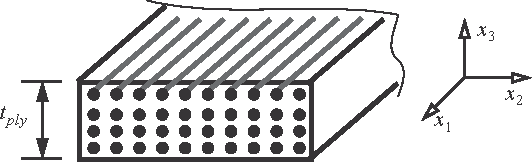
\includegraphics{Figure_8-1.pdf}}{\caption{Unidirectional lamina of a continuous fiber composite.}\label{fig8.1}}

\begin{quote}
The advantage of polymer-composites aerospace structures are many:
They weigh less than equivalent-strength aluminum, do not corrode
or fatigue, require less maintenance, and reduce the need for
drilled holes and parts. Composite parts generally cost more than
equivalent metal parts, but that premium is decreasing. And the
cost premium is offset by operating savings in fuel and
maintenance (Canaday, 2015).
\end{quote}

\subsection{Material law in principal directions}\label{sec8.1.1}

Fiber-reinforced composites are usually treated as a linear
elastic material with orthotropic material properties in the
material principal directions (i.e directions parallel and
perpendicular to the fibers). In a right-handed Cartesian system
denoted by $x_1$-$x_2$-$x_3$, let the $x_1$-axis be parallel to
the fibers, the $x_2$-axis be transverse to the fibers, and the
$x_3$-axis be parallel to the thickness of the lamina. (Also,
refer to discussion with respect to eq. (\ref{eqA.131}) in the
appendix.) In the discussion of the material law, it is convenient
to use a contracted notation for strain components and the
corresponding stress components. The contracted notation defines
the 6-by-1 engineering strain vector in principal material
directions as
\begin{align}\label{eq8.1}
\left\{\gamma_m \right\}=\left[\begin{array}{@{}llllll@{}} \varepsilon_{11} & \varepsilon_{22} & \varepsilon_{33} & \gamma_{23} & \gamma_{31} & \gamma_{12} \end{array}\right]^{T} ,
\end{align}
where the normal strains are denoted by $\varepsilon_{11},
\varepsilon_{22}$, and $\varepsilon_{33}$, and the shear strains are
denoted by $\gamma_{23}, \gamma_{31}$, and $\gamma_{12}$. The
corresponding 6-by-1 stress vector in principal material
directions is
\begin{align}\label{eq8.2}
\left\{\sigma_{m}\right\}=\left[\begin{array}{@{}llllll@{}}
\sigma_{11} & \sigma_{22} & \sigma_{33} & \sigma_{23} &
\sigma_{31} & \sigma_{12} \end{array}\right]^{T} ,
\end{align}
where the normal stresses are denoted by $\sigma_{11},
\sigma_{22}$, and $\sigma_{33}$, and the shear stresses are
denoted by $\sigma_{23}, \sigma_{31}$, and $\sigma_{12}$. See
figure~\ref{fig8.2}.

\vspace*{-12pt}
\processfigure[H]{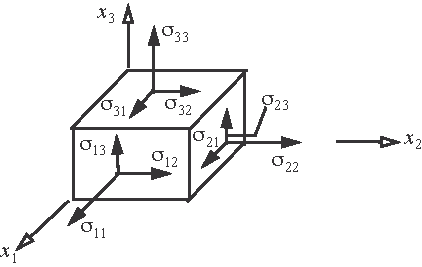
\includegraphics{Figure_8-2.pdf}}{\caption{Stresses in material principal directions.}\label{fig8.2}}
\vspace*{-12pt}

Hooke's law for an orthotropic material in the contracted notation
is
\begin{align}\label{eq8.3}
\left[\begin{array}{@{}l@{}} \varepsilon_{11}\\
\varepsilon_{22}\\
\varepsilon_{33}\\
\gamma_{23}\\
\gamma_{31}\\
\gamma_{12}
\end{array}\right]=\underbrace{\left[\begin{array}{@{}cccccc@{}}
C_{11} & C_{12} & C_{13} & 0 & 0 & 0\\
C_{21} & C_{22} & C_{23} &
0 & 0 & 0\\
C_{31} & C_{32} & C_{33} & 0 & 0 & 0\\
0 & 0 & 0 &
C_{44} & 0 & 0\\
0 & 0 & 0 & 0 & C_{55} & 0\\
0 & 0 & 0 & 0 & 0
& C_{66} \end{array}\right]}_{[C]}\left[\begin{array}{@{}l@{}}
\sigma_{11}\\
\sigma_{22}\\
\sigma_{33}\\
\sigma_{23}\\
\sigma_{31}\\
\sigma_{12} \end{array}\right] ,
\end{align}
in which [$C$] is the symmetric 6X6 compliance matrix. The
non-zero elements of the compliance matrix in terms of engineering
constants are
\begin{align}
C_{11}=\frac{1}{E_{1}} \quad C_{22}=\frac{1}{E_{2}} \quad C_{33}=\frac{1}{E_{3}} \quad C_{44}=\frac{1}{G_{23}} \quad C_{55}=\frac{1}{G_{13}} \quad C_{66}=\frac{1}{G_{12}}\mbox{, and}\label{eq8.4}
\end{align}
\pagebreak
\begin{gather}
\begin{split}\label{eq8.5}
C_{21}=-v_{21}/ E_{1}=C_{12}=-v_{12}/ E_{2}\\
C_{31}=-v_{31}/ E_{1}=C_{13}=-v_{13}/ E_{3}\\
C_{32}=-v_{32}/ E_{2}=C_{23}=-v_{23}/ E_{3}
\end{split}.
\end{gather}
The nine independent engineering constants are described as
follows:
\begin{itemize}
\item Moduli of elasticity in the fiber direction, transverse direction, and thickness direction are denoted by $E_1$, $E_2$, and $E_3$, respectively.

\item The principal Poisson's ratios are $\nu_{21}$, $\nu_{31}$, and $\nu_{32}$.

\item Shear moduli in the 2-3 plane, 3-1 plane, and 1-2 plane are denoted by $G_{23}$, $G_{31}$, and $G_{12}$, respectively.
\end{itemize}

\noindent The three minor Poisson's ratios, $\nu_{12}$,
$\nu_{13}$, and $\nu_{23}$, are determined from symmetry of the
compliance matrix. Material characterization tests are conducted
to measure the nine independent engineering constants. However,
the most accurate measurements are made for the in-plane
properties $E_1$, $E_2$, $\nu_{21}$, and $G_{12}$.

\subsection{Compliance matrix in bar coordinate directions}\label{sec8.1.2}

Consider the thin-walled bar, or beam, analysis presented in
article \ref{sec3.2} to article \ref{sec3.5}. Instead of a the
wall composed of a homogeneous, linear elastic material as in
article \ref{sec3.7}, we now take the wall to be composed of a fibrous
composite material. The fibers are parallel and contained in thin
layers, or lamina, that are normal to the thickness coordinate
direction $\zeta$ of the wall. Within a lamina the bar contour
coordinate direction $s$, and longitudinal direction $z$, are not,
in general, aligned with the material principal coordinate
directions $x_1$ and $x_2$. Define a positive angle $\varphi$ by
the counterclockwise rotation from the positive $z$-axis to the
positive $x_1$-axis as shown in figure~\ref{fig8.3}.

\processfigure{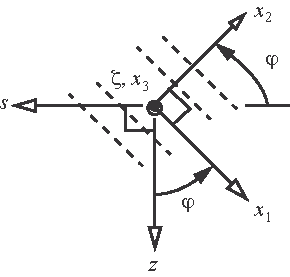
\includegraphics{Figure_8-3.pdf}}{\caption{Material principal directions $x_\textbf{1}$, $x_\textbf{2}$, and $x_\textbf{3}$ with respect to bar axes $s$, $z$, and $\zeta$.}\label{fig8.3}}

\noindent The direction cosines between the principal material coordinate
directions $x_1$-$x_2$-$x_3$ and the bar coordinate directions
$s$-$z$-$\zeta$ are listed in table~\ref{tab8.1}.

%Table 8.1
\begin{table}[!h]
\processtable{Direction cosines\label{tab8.1}}{\begin{tabular}{@{}l|lll@{}}
\toprule\\[-15.5pt]
& & & \\[-6pt]
\colhead{\textbf{s}} & \colhead{\textit{\textbf{z}}} & \colhead{$\zeta$}\\
 & & & \\[-8pt]
\midrule\\[-15pt]
 & & & \\[-8.5pt]
$x_1$ & $\cos (90^{\circ}+\varphi) $ & $\cos\varphi$ & 0\\
$x_2$ & $\cos (180^{\circ}-\varphi)$ & $\cos(90^{\circ}+\varphi)$ & 0\\
$x_3$ & 0 & 0 & 1\\[-7pt]
& & & \\[-3.5pt]
\botrule
\end{tabular}}{}
\vspace*{-1pc}
\end{table}

\noindent Let $ m=\cos \varphi $ and $ n=\sin \varphi $. Then, the
matrix relations between the coordinate directions are written as
\begin{align}\label{eq8.6}
\left[\begin{array}{@{}l@{}} x_{1}\\
x_{2}\\
x_{3}
\end{array}\right]=\underbrace{\left[\begin{array}{@{}ccc@{}} -n &
m & 0\\
-m & -n & 0\\
0 & 0 & 1
\end{array}\right]}_{[\lambda]}\left[\begin{array}{@{}l@{}} s\\
z\\
\zeta \end{array}\right] \text { and
}\left[\begin{array}{@{}c@{}} s\\
z\\
\zeta
\end{array}\right]=\underbrace{\left[\begin{array}{@{}ccc@{}} -n &
-m & 0\\
m & -n & 0\\
0 & 0 & 1
\end{array}\right]}_{[\lambda]^{T}}\left[\begin{array}{@{}l@{}}
x_{1}\\
x_{2}\\
x_{3} \end{array}\right]\!.
\end{align}
Matrix [$\lambda$] is an orthogonal matrix so that
$[\lambda][\lambda]^{T}=[\lambda]^{T}[\lambda]=[I] $, and
$\operatorname{Det}[\lambda]=1$. In the material coordinate
directions the symmetric, Cartesian strain tensor is denoted by
the 3X3 matrix $[\varepsilon]$, and the symmetric, stress tensor
is denoted by the 3X3 matrix $[\sigma]$. The elements of these
matrices are
\begin{align}\label{eq8.7}
[\varepsilon]=\left[\begin{array}{@{}ccc@{}} \varepsilon_{11} &
\gamma_{12}/ 2 & \gamma_{13}/ 2\\
\gamma_{12}/ 2 &
\varepsilon_{22} & \gamma_{23}/ 2\\
\gamma_{13}/ 2 &
\gamma_{23}/ 2 & \varepsilon_{33} \end{array}\right] \mbox{ and }
[\sigma]=\left[\begin{array}{@{}lll@{}} \sigma_{11} & \sigma_{12}
&
\sigma_{13}\\
\sigma_{12} & \sigma_{22} & \sigma_{23}\\
\sigma_{13} & \sigma_{23} & \sigma_{33}
\end{array}\right].
\end{align}
In the bar coordinate directions, the strain matrix
$[\varepsilon^{\prime}]$ and stress matrix $[\sigma^{\prime}]$ are
denoted by
\begin{align}\label{eq8.8}
\left[\varepsilon^{\prime}\right]=\left[\begin{array}{@{}ccc@{}}
\varepsilon_{s s} & \gamma_{z s}/ 2 & \gamma_{_{\zeta s}}/ 2\\
\gamma_{z s}/ 2 & \varepsilon_{z z} & \gamma_{\zeta z}/ 2\\
\gamma_{\zeta_{s}}/ 2 & \gamma_{\zeta z}/ 2 & \varepsilon_{\zeta
\zeta} \end{array}\right] \mbox{ and }
\left[\sigma^{\prime}\right]=\left[\begin{array}{@{}ccc@{}}
\sigma_{s s} & \sigma_{z s} & \sigma_{\zeta s}\\
\sigma_{z s} &
\sigma_{z z} & \sigma_{\zeta z}\\
\sigma_{\zeta s} &
\sigma_{\zeta z} & \sigma_{\zeta \zeta} \end{array}\right].
\end{align}
From eq. (\ref{eqA.63}) and eq. (\ref{eqA.65}) in the appendix the
transformation relations between the Cartesian strain matrices are
\begin{align}\label{eq8.9}
\left[\varepsilon^{\prime}\right]=[\lambda][\varepsilon][\lambda]^{T}
\mbox{ and }
[\varepsilon]=[\lambda]^{T}\left[\varepsilon^{\prime}\right][\lambda].
\end{align}
From eq. (\ref{eqA.96}) and eq. (\ref{eqA.97}) in the appendix the
transformation relations between the stress matrices are
\begin{align}\label{eq8.10}
\left[\sigma^{\prime}\right]=[\lambda][\sigma][\lambda]^{T}\mbox{
and } [\sigma]=[\lambda]^{T}\left[\sigma^{\prime}\right][\lambda].
\end{align}
After performing the matrix operations indicated for the strain
matrices (\ref{eq8.9}), we can establish the contracted notation
for the transformation of the strain vectors. The results are as
follows:
\begin{align}
\left[\begin{array}{@{}l@{}} \varepsilon_{s s}\\
\varepsilon_{z z}\\
\varepsilon_{\zeta \zeta}\\
\gamma_{z \zeta}\\
\gamma_{\zeta s}\\
\gamma_{s z} \end{array}\right]=\underbrace{\left[\begin{array}{@{}cccccc@{}} n^{2} & m^{2} & 0 & 0 & 0 & -m n\\
m^{2} & n^{2} & 0 & 0 & 0 & m n\\
0 & 0 & 1 & 0 & 0 & 0\\
0 & 0 & 0 & -n & -m & 0\\
0 & 0 & 0 & m & -n & 0\\
2 m n & -2 m n & 0 & 0 & 0 & -m^{2}+n^{2} \end{array}\right]}_{\left[\begin{array}{@{}c@{}} T_{\varepsilon 1} \end{array}\right]}\left[\begin{array}{@{}l@{}} \varepsilon_{11}\\
\varepsilon_{22}\\
\varepsilon_{33}\\
\gamma_{23}\\
\gamma_{31}\\
\gamma_{12} \end{array}\right]\label{eq8.11}\\
\left[\begin{array}{@{}l@{}} \varepsilon_{11}\\
\varepsilon_{22}\\
\varepsilon_{33}\\
\gamma_{23}\\
\gamma_{31}\\
\gamma_{12}
\end{array}\right]=\underbrace{\left[\begin{array}{@{}cccccc@{}} n^{2} &
m^{2} & 0 & 0 & 0 & m n\\
m^{2} & n^{2} & 0 & 0 & 0 & -m n\\
0 &
0 & 1 & 0 & 0 & 0\\
0 & 0 & 0 & -n & m & 0\\
0 & 0 & 0 & -m & -n
& 0\\
-2 m n & 2 m n & 0 & 0 & 0 & -m^{2}+n^{2}
\end{array}\right]}_{\left[\begin{array}{@{}c@{}}
T_{\varepsilon 2}
\end{array}\right]}\left[\begin{array}{@{}c@{}} \varepsilon_{s s}\\
\varepsilon_{z z}\\
\varepsilon_{\zeta \zeta}\\
\gamma_{z
\zeta}\\
\gamma_{\zeta s}\\
\gamma_{s z} \end{array}\right].\label{eq8.12}
\end{align}
Note that $\operatorname{Det}\left[T_{\varepsilon
1}\right]=\operatorname{Det}\left[T_{\varepsilon_{2}}\right]=1$,
and $\left[T_{\varepsilon 1}\right]\left[T_{\varepsilon
2}\right]=[I]$. That is, $ \left[T_{\mathrm{\varepsilon}
2}\right]=\left[T_{\mathrm{s} 1}\right]^{-1}$. After performing
the matrix operations indicated for the stress matrices
(\ref{eq8.10}), we can establish the contracted notation for the
transformation of the stress vectors. The results are as follows:
\begin{gather}
\left[\begin{array}{@{}c@{}} \sigma_{s s}\\
\sigma_{z z}\\
\sigma_{\zeta \zeta}\\
\sigma_{z \zeta}\\
\sigma_{\zeta s}\\
\sigma_{s z}
\end{array}\right]=\underbrace{\left[\begin{array}{@{}cccccc@{}}
n^{2} & m^{2} & 0 & 0 & 0 & -2 m n\\
m^{2} & n^{2} & 0 & 0 & 0 &
2 m n\\
0 & 0 & 1 & 0 & 0 & 0\\
0 & 0 & 0 & -n & -m & 0\\
0 & 0
& 0 & m & -n & 0\\
m n & -m n & 0 & 0 & 0 & -m^{2}+n^{2}
\end{array}\right]}_{\left[\begin{array}{@{}cccccc@{}} T_{\sigma
1} \end{array}\right]}\left[\begin{array}{@{}l@{}} \sigma_{11}\\
\sigma_{22}\\
\sigma_{33}\\
\sigma_{23}\\
\sigma_{31}\\
\sigma_{12} \end{array}\right]\label{eq8.13}\\[6pt]
\left[\begin{array}{@{}l@{}} \sigma_{11}\\
\sigma_{22}\\
\sigma_{33}\\
\sigma_{23}\\
\sigma_{31}\\
\sigma_{12}
\end{array}\right]=\underbrace{\left[\begin{array}{@{}cccccc@{}}
n^{2} & m^{2} & 0 & 0 & 0 & 2 m n\\
m^{2} & n^{2} & 0 & 0 & 0 &
-2 m n\\
0 & 0 & 1 & 0 & 0 & 0\\
0 & 0 & 0 & -n & m & 0\\
0 & 0 & 0 & -m & -n & 0\\
-m n & m n & 0 & 0 & 0 & -m^{2}+n^{2}
\end{array}\right]}_{\left[T_{\sigma 2}\right].}
\left[\begin{array}{@{}l@{}} \sigma_{s s}\\
\sigma_{z z}\\
\sigma_{\zeta \zeta}\\
\sigma_{z \zeta}\\
\sigma_{\zeta s}\\
\sigma_{s z}
\end{array}\right]\label{eq8.14}
\end{gather}
Note that $\operatorname{Det}\left[T_{\sigma
1}\right]=\operatorname{Det}\left[T_{\sigma 2}\right]=1$, and
$\left[T_{\sigma 1}\right]\left[T_{\sigma 2}\right]=[I]$. That is,
$ \left[T_{\sigma 2}\right]=\left[T_{\sigma 1}\right]^{-1}$.
Additionally, from the foregoing eqs. (\ref{eq8.11}) to
(\ref{eq8.14}) the following matrix relations can be shown:
\begin{align}\label{eq8.15}
\left[T_{\mathrm{\varepsilon}1}\right]^{T}=\left[T_{\sigma 2}\right]\mbox{
and }\left[T_{\varepsilon 2}\right]^{T}=\left[T_{\sigma 1}\right]
\end{align}
The elements of the 6X6 matrices in eq.~(\ref{eq8.15}) are as
follows:
\begin{align*}
\underbrace{\left[\begin{array}{@{}cccccc@{}}
n^{2} & m^{2} & 0 & 0 & 0 & -m n\\
m^{2} & n^{2} & 0 & 0 & 0 & m n\\
0 & 0 & 1 & 0 & 0 & 0\\
0 & 0 & 0 & -n & -m & 0\\
0 & 0 & 0 & m & -n & 0\\
2 m n & -2 m n & 0 & 0 & 0 & -m^{2}+n^{2}
\end{array}\right]^T}_{\left[T_{\varepsilon 1}\right]^{T}}
=\underbrace{\left[\begin{array}{@{}cccccc@{}}
n^{2} & m^{2} & 0 & 0 & 0 & 2 m n\\
m^{2} & n^{2} & 0 & 0 & 0 & -2 m n\\
0 & 0 & 1 & 0 & 0 & 0\\
0 & 0 & 0 & -n & m & 0\\
0 & 0 & 0 & -m & -n & 0\\
-m n & m n & 0 & 0 & 0 & -m^{2}+n^{2}
\end{array}\right]}_{\left[T_{\sigma
2}\right]}\\
\mbox{, and }\\
\underbrace{\left[\begin{array}{@{}cccccc@{}}
n^{2} & m^{2} & 0 & 0 & 0 & m n\\
m^{2} & n^{2} & 0 & 0 & 0 & -m n\\
0 & 0 & 1 & 0 & 0 & 0\\
0 & 0 & 0 & -n & m & 0\\
0 & 0 & 0 & -m & -n & 0\\
-2 m n & 2 m n & 0 & 0 & 0 & -m^{2}+n^{2}
\end{array}\right]^T}_{\left[T_{\varepsilon 2}\right]^{T}}
=\underbrace{\left[\begin{array}{@{}cccccc@{}}
n^{2} & m^{2} & 0 & 0 & 0 & -2 m n\\
m^{2} & n^{2} & 0 & 0 & 0 & 2 m n\\
0 & 0 & 1 & 0 & 0 & 0\\
0 & 0 & 0 & -n & -m & 0\\
0 & 0 & 0 & m & -n & 0\\
m n & -m n & 0 & 0 & 0 & -m^{2}+n^{2}
\end{array}\right]}_{\left[T_{\sigma
1}\right]}.
\end{align*}

To determine the off-axis compliance material law we pre-multiply
the on-axis material law (\ref{eq8.3}) by matrix $[T_{\varepsilon
1}]$, followed by substituting of eq.~(\ref{eq8.14}) for the
on-axis stresses on the right-hand side of eq.~(\ref{eq8.3}). Use
the fact that $[T_{\varepsilon 1}]^{T}=\left[\begin{array}{@{}l@{}}
T_{\sigma 2}\end{array}\right] $ from eq.~(\ref{eq8.15}). Denote
the 6X6 off-axis compliance matrix by $\left[C^{\prime}\right]$
and we find that $ \left[C^{\prime}\right]=\left[T_{\varepsilon
1}\right][C]\left[T_{\varepsilon 1}\right]^{T}$. The form of the
off-axis material law is
\begin{align}\label{eq8.16}
\left[\begin{array}{@{}l@{}} \varepsilon_{s s}\\[4pt]
\varepsilon_{z
z}\\[4pt]
\varepsilon_{\zeta \zeta}\\[4pt]
\gamma_{z \zeta}\\[4pt]
\gamma_{\zeta s}\\[4pt]
\gamma_{s z}
\end{array}\right]=\left[\begin{array}{@{}cccccc@{}}
C_{11}^{\prime} & C_{12}^{\prime} & C_{13}^{\prime} & 0 & 0 &
C_{16}^{\prime}\\[4pt]
C_{21}^{\prime} & C_{22}^{\prime} &
C_{23}^{\prime} & 0 & 0 & C_{26}^{\prime}\\[4pt]
C_{31}^{\prime} &
C_{32}^{\prime} & C_{33}^{\prime} & 0 & 0 & C_{36}^{\prime}\\[4pt]
0 &
0 & 0 & C_{44}^{\prime} & C_{45}^{\prime} & 0\\[4pt]
0 & 0 & 0 &
C_{54}^{\prime} & C_{55}^{\prime} & 0\\[4pt]
C_{61}^{\prime} &
C_{62}^{\prime} & C_{63}^{\prime} & 0 & 0 & C_{66}^{\prime}
\end{array}\right]\left[\begin{array}{@{}c@{}} \sigma_{s s}\\[4pt]
\sigma_{z z}\\[4pt]
\sigma_{\zeta \zeta}\\[4pt]
\sigma_{z \zeta}\\[4pt]
\sigma_{\zeta s}\\[4pt]
\sigma_{s z} \end{array}\right].
\end{align}
Matrix $\left[C^{\prime}\right]$ is symmetric with the compliance
coefficients in terms of the engineering constants and the
directions cosines given by eq.~(\ref{eq8.17}) to (\ref{eq8.23})
below.
\begin{gather}
C_{11}^{\prime}=\frac{m^{4}}{E_{2}}+\frac{m^{2}
n^{2}}{G_{12}}+\frac{n^{4}-2 m^{2} n^{2} v_{21}}{E_{1}} \quad
C_{21}^{\prime}=C_{12}^{\prime}=\frac{m^{2}
n^{2}\left(G_{12}-E_{2}\right)}{E_{2} G_{12}}+\frac{m^{2}
n^{2}-\left(m^{4}+n^{4}\right) v_{21}}{E_{1}}\label{eq8.17}\\[-3pt]
C_{31}^{\prime}=C_{13}^{\prime}=\frac{-n^{2}
{v}_{31}}{E_{1}}-\frac{m^{2} {v}_{32}}{E_{2}} \quad
C_{61}^{\prime}=C_{16}^{\prime}=m n\left(\frac{-2
m^{2}}{E_{2}}+\frac{m^{2}-n^{2}}{G_{12}}-\frac{2 m^{2}
{v}_{21}}{E_{1}}+\frac{2
n^{2}\left(1+v_{21}\right)}{E_{1}}\right)\label{eq8.18}\\[-3pt]
C_{22}^{\prime}=\frac{m^{2}
n^{2}}{G_{12}}+\frac{n^{4}}{E_{2}}+\frac{m^{4}-2 m^{2} n^{2}
{v}_{21}}{E_{1}} \quad
C_{23}^{\prime}=C_{32}^{\prime}=\frac{-m^{2}
{v}_{31}}{E_{1}}-\frac{n^{2}
{v}_{32}}{E_{2}}\label{eq8.19}\\[-3pt]
C_{26}^{\prime}=C_{62}^{\prime}=m n\left(\frac{-2
n^{2}}{E_{2}}+\frac{n^{2}-m^{2}}{G_{12}}+\frac{2
m^{2}\left(1+v_{21}\right)-2 n^{2}
v_{21}}{E_{1}}\right)\label{eq8.20}\\[-3pt]
C_{33}^{\prime}=\frac{1}{E_{3}} \quad
C_{63}^{\prime}=C_{36}^{\prime}=2 m
n\left(\frac{v_{32}}{E_{2}}-\frac{v_{31}}{E_{1}}\right)\label{eq8.21}\\[-3pt]
C^{\prime}_{44}=\frac{m^{2}}{G_{13}}+\frac{n^{2}}{G_{23}} \quad
C_{54}^{\prime}=C_{45}^{\prime}=m
n\left(\frac{1}{G_{13}}-\frac{1}{G_{23}}\right) \quad
C_{55}^{\prime}=\frac{m^{2}}{G_{23}}+\frac{n^{2}}{G_{13}}\label{eq8.22}\\[-3pt]
C_{66}^{\prime}=\frac{\left(m^{2}-n^{2}\right)^{2}}{G_{12}}+\frac{4
m^{2} n^{2}\left(E_{1}+\left(1+2 v_{21}\right) E_{2}\right)}{E_{1}
E_{2}}.\label{eq8.23}
\end{gather}

\subsection{Plane stress}\label{sec8.1.3}

Since composites used in many structural applications are thin
plates or thin shells, the assumption of a plane stress state as
used plate and shell theory is also made for a composite plate. In
figure~\ref{fig8.2} the in-plane stress components are
$\sigma_{11}$, $\sigma_{22}$, and $\sigma_{12}$. Thus, the
following stress components are assumed negligible with respect to
the in-plane stress components and set equal to zero in
eq.~(\ref{eq8.3}):
\begin{align}\label{eq8.24}
\sigma_{33}=\sigma_{31}=\sigma_{13}=\sigma_{32}=\sigma_{23}=0.
\end{align}
Hence, the compliance form of the orthotropic material law for a
unidirectional lamina subject to plane stress is
\begin{align}\label{eq8.25}
\left[\begin{array}{@{}l@{}} \varepsilon_{11}\\
\varepsilon_{22}\\
\gamma_{12}
\end{array}\right]=\underbrace{\left[\begin{array}{@{}ccc@{}}
C_{11} & C_{12} & 0\\
C_{21} & C_{22} & 0\\
0 & 0 & C_{66}
\end{array}\right]}_{[C]}\left[\begin{array}{@{}l@{}} \sigma_{11}\\
\sigma_{22}\\
\sigma_{12}
\end{array}\right]=\left[\begin{array}{@{}ccc@{}} 1/ E_{1} &
-v_{12}/ E_{2} & 0\\
-v_{21}/ E_{1} & 1/ E_{2} & 0\\
0 & 0 &
1/ G_{12} \end{array}\right]\left[\begin{array}{@{}l@{}}
\sigma_{11}\\
\sigma_{22}\\
\sigma_{12} \end{array}\right] ,
\end{align}
and the thickness normal strain is
\begin{align}\label{eq8.26}
\varepsilon_{33}=C_{31} \sigma_{11}+C_{32} \sigma_{22}.
\end{align}
\vspace*{1pt}\vspace*{-8pt}
\clearpage

\noindent The stress-strain form of the material law (\ref{eq8.25}) is
written as
\begin{align}\label{eq8.27}
\left[\begin{array}{@{}l@{}} \sigma_{11}\\
\sigma_{22}\\
\sigma_{12}
\end{array}\right]=\underbrace{\left[\begin{array}{@{}ccc@{}}
Q_{11} & Q_{12} & 0\\
Q_{21} & Q_{22} & 0\\
0 & 0 & Q_{66}
\end{array}\right]}_{[Q]}\left[\begin{array}{@{}l@{}}
\varepsilon_{11}\\
\varepsilon_{22}\\
\gamma_{12}
\end{array}\right]=\left[\begin{array}{@{}ccc@{}} E_{1}
/\left(1-v_{21} v_{12}\right) & \left(v_{12} E_{1}\right)
/\left(1-v_{21} v_{12}\right) & 0\\
\left(v_{21} E_{2}\right)
/\left(1-v_{21} v_{12}\right) & E_{2}/\left(1-v_{21}
v_{12}\right) & 0\\
0 & 0 & G_{12}
\end{array}\right]\left[\begin{array}{@{}l@{}} \varepsilon_{11}\\
\varepsilon_{22}\\
\gamma_{12} \end{array}\right],
\end{align}
where the matrix [$Q$] is called the reduced stiffness matrix.
Matrix [$Q$] is symmetric since $v_{21} E_{2}=v_{12} E_{1}$.
(refer to eq.~(\ref{eq8.5})). It follows from eq.~(\ref{eq8.3})
that the transverse shear strains $\gamma_{23}=\gamma_{31}=0$,
which leads to transverse shear strains
$\gamma_{z\zeta}=\gamma_{\zeta s}=0$ by eq.~(\ref{eq8.11}). Also,
the normal strain $\varepsilon_{\zeta\zeta}=\varepsilon_{33}$. From
eq.~(\ref{eq8.13}) the stresses $ \sigma_{\zeta \zeta}=\sigma_{z
\zeta}=\sigma_{\zeta s}=0$.

Transform eq.~(\ref{eq8.27}) to an off-axis material law as
follows: For plane stress the stress transformation equation
(\ref{eq8.13}) reduces to
\begin{align}\label{eq8.28}
\left[\begin{array}{@{}c@{}} \sigma_{s s}\\
\sigma_{z z}\\
\sigma_{s z}
\end{array}\right]=\underbrace{\left[\begin{array}{@{}ccc@{}}
n^{2} & m^{2} & -2 m n\\
m^{2} & n^{2} & 2 m n\\
m n & -m n &
\left(-m^{2}+n^{2}\right)
\end{array}\right]}_{\left[\begin{array}{@{}c@{}} T_{\sigma 1}
\end{array}\right]}\left[\begin{array}{@{}l@{}} \sigma_{11}\\
\sigma_{22}\\
\sigma_{12} \end{array}\right] ,
\end{align}
and the strain transformation eq.~(\ref{eq8.11}) reduces to
\begin{align}\label{eq8.29}
\left[\begin{array}{@{}l@{}} \varepsilon_{11}\\
\varepsilon_{22}\\
\gamma_{12}
\end{array}\right]=\underbrace{\left[\begin{array}{@{}ccc@{}}
n^{2} & m^{2} & m n\\
m^{2} & n^{2} & -m n\\
-2 m n & 2mn & \left(-m^{2}+n^{2}\right)\end{array}\right]}_{\left[\begin{array}{@{}c@{}}T_{\varepsilon2}\end{array}\right]}\left[\begin{array}{@{}c@{}} \varepsilon_{ss}\\
\varepsilon_{z z}\\
\gamma_{s z} \end{array}\right].
\end{align}
Pre-multiply eq.~(\ref{eq8.27}) $ \left[T_{\sigma 1}\right]$, and
substitute the strain transformation eq.~(\ref{eq8.29}) on the
right-hand side of eq.~(\ref{eq8.27}). Use the fact that $
\left[T_{\varepsilon 2}\right]=\left[T_{\sigma 1}\right]^{T} $
from eq.~(\ref{eq8.15}). These matrix manipulations result in the
off-axis material law in plane stress given by
\begin{align}\label{eq8.30}
\left[\begin{array}{@{}l@{}} \sigma_{s s}\\
\sigma_{z z}\\
\sigma_{s z} \end{array}\right]=\left[\begin{array}{@{}l@{}}
\bar{Q} \end{array}\right]\left[\begin{array}{@{}l@{}}
\varepsilon_{s s}\\
\varepsilon_{z z}\\
\gamma_{s z}
\end{array}\right]=\left[\begin{array}{@{}lll@{}} \bar{Q}_{11} &
\bar{Q}_{12} & \bar{Q}_{16}\\
\bar{Q}_{21} & \bar{Q}_{22} &
\bar{Q}_{26}\\
\bar{Q}_{61} & \bar{Q}_{62} & \bar{Q}_{66}
\end{array}\right]\left[\begin{array}{@{}l@{}} \varepsilon_{s s}\\
\varepsilon_{z z}\\
\gamma_{s z} \end{array}\right] ,
\end{align}
where the transformed reduced stiffness matrix is given by $
[\bar{Q}]=\left[T_{\sigma 1}\right][Q]\left[T_{\sigma
1}\right]^{T} $. Since the on-axis reduced stiffness matrix $ [Q]
$ is symmetric, it follows from these matrix relations that the
transformed stiffness matrix is symmetric
($[\bar{Q}]^{T}=[\bar{Q}]$). Elements of the transformed reduced
stiffness matrix in terms of the reduced matrix elements are given
by
\begin{align}\label{eq8.31}
\left[\begin{array}{@{}l@{}} \bar{Q}_{11}\\
\bar{Q}_{22}\\
\bar{Q}_{21}\\
\bar{Q}_{66}\\
\bar{Q}_{16}\\
\bar{Q}_{26}
\end{array}\right]=\left[\begin{array}{@{}cccc@{}} n^{4} & m^{4} &
2 m^{2} n^{2} & 4 m^{2} n^{2}\\
m^{4} & n^{4} & 2 m^{2} n^{2} & 4
m^{2} n^{2}\\
m^{2} n^{2} & m^{2} n^{2} &
\left(m^{4}+n^{4}\right) & -4 m^{2} n^{2}\\
m^{2} n^{2} & m^{2}
n^{2} & -2 m^{2} n^{2} & \left(-m^{2}+n^{2}\right)^{2}\\
m n^{3}
& -m^{3} n & m n\left(m^{2}-n^{2}\right) & 2 m
n\left(m^{2}-n^{2}\right)\\
m^{3} n & -m n^{3} & -m
n\left(m^{2}-n^{2}\right) & -2 m n\left(m^{2}-n^{2}\right)
\end{array}\right]\left[\begin{array}{@{}l@{}} Q_{11}\\
Q_{22}\\
Q_{21}\\
Q_{66} \end{array}\right].
\end{align}

\subsection{Nomenclature of composite materials}\label{sec8.1.4}



Composite materials are identified by the name of the fiber
followed by the name of the matrix. For example, AS4/3501-6
denotes the carbon fiber AS4 and the epoxy matrix 3501-6. The data
in table~\ref{tab8.2} is taken from Herakovich (1998, p.~\pageref{Herakovich}), and it lists
typical properties for AS4/3501-6 and T300/5208 carbon
fiber-reinforced epoxy composites.


%Table 8.2
\begin{table}[!h]
\processtable{Material properties of selected CFRP lamina\label{tab8.2}}
{\begin{tabular}{@{}llll@{}}\toprule
\colhead{\textbf{Property}} & \colhead{\textbf{Units}} & \colhead{\textbf{AS4/3501-6}} &
\colhead{\textbf{T300/5208}}\\
\midrule
 Axial modulus $E_1$ & GPa & 148 & 132\\
 & Msi & \phantom{0}21.5 & \phantom{0}19.2\\
 Transverse modulus $E_2$ & GPa & \phantom{0}10.5 & \phantom{0}10.8\\
 & Msi & \phantom{00}1.46 & \phantom{00}1.56\\
 Major Poisson's ratio $\nu_{21}$ & dimensionless & \phantom{00}0.30 & \phantom{00}0.24\\
 Major Poisson's ratio $\nu_{23}$ & dimensionless & \phantom{00}0.59 & \phantom{00}0.59\\
 Shear modulus $G_{12}$ & GPa & \phantom{00}5.61 & \phantom{00}5.65\\
 & Msi & \phantom{00}0.81 & \phantom{00}0.82\\
 Shear modulus $G_{23}$ & GPa & \phantom{00}3.17 & \phantom{00}3.38\\
 & Msi & \phantom{00}0.46 & \phantom{00}0.49\\
 Density & \textit{g/cm}$^3$ & \phantom{00}1.52 & \phantom{00}1.54\\
 & lb./in.$^3$ & \phantom{00}0.055 & \phantom{00}0.056\\
 Ply thickness $t_{ply}$ & mm & \phantom{00}0.127 & \phantom{00}0.127\\
 & in. & \phantom{00}0.005 & \phantom{00}0.005\\
 Fiber volume fraction $V_f$ & dimensionless & \phantom{00}0.62 & \phantom{00}0.62\\
 \botrule
\end{tabular}}{}
\vspace*{-12pt}
\end{table}

\begin{example*}[Transformed reduced stiffness matrix for
an off-axis ply]\label{ex8.1}Determine the transformed reduced
stiffness matrix of T300/5208 carbon/epoxy for a 30-degree
off-axis lamina in U.S. customary units.

\subsubsection{Solution.} From table \ref{tab8.2}
$E_{1}=19.2\,\mathrm{Msi}$, $E_{2}=1.56\,\mathrm{Msi}$,
$v_{21}=0.24$, and $G_{12}=0.82\,\mathrm{Msi}$. The minor Poisson's
ratio is $v_{12}=0.24[(1.56\,\mathrm{Msi})
/(19.2\,\mathrm{Msi})]=0.0195$. The reduced stiffness matrix is
computed from eq.~(\ref{eq8.30}) and eq.~(\ref{eq8.31}); i.e.,
\begin{align}\label{ex8.1a}
[Q]=\left[\begin{array}{@{}ccc@{}} 19.3 & 0.376 & 0\\
0.376 &
1.57 & 0\\
0 & 0 & 0.82 \end{array}\right]\,\mathrm{Msi}.\tag{a}
\end{align}
The transformed reduced stiffness matrix is given by $
[\bar{Q}]=\left[T_{\sigma 1}\right][Q]\left[T_{\sigma
1}\right]^{T}$\!, the reduced stiffness by eq.~(\ref{eq8.27}), and
the transform matrix $ \left[T_{\sigma 1}\right] $ by
eq.~(\ref{eq8.28}). The matrix product is
\begin{align}\label{ex8.1b}
[\bar{Q}]=\left[\begin{array}{@{}ccc@{}} 1/ 4 & 3/ 4 & -\sqrt{3}
/ 2\\
3/ 4 & 1/ 4 & \sqrt{3}/ 2\\
\sqrt{3}/ 4 & -\sqrt{3}/
4 & -1/ 2
\end{array}\right]\left[\begin{array}{@{}ccc@{}} 19.3 & 0.376 & 0\\
0.376 & 1.57 & 0\\
0 & 0 & 0.82
\end{array}\right]\left[\begin{array}{@{}ccc@{}} 1/ 4 & 3/ 4 &
\sqrt{3}/ 4\\
3/ 4 & 1/ 4 & -\sqrt{3}/ 4\\
-\sqrt{3}/ 2 &
\sqrt{3}/ 2 & -1/ 2 \end{array}\right],\tag{b}
\end{align}
and the result is\pagebreak
\begin{align}\label{ex8.1c}
[\bar{Q}]=\left[\begin{array}{@{}lll@{}} 2.84537 & 3.53313 & 2.01589\\
3.53313 & 11.7104 & 5.66142\\
2.01589 & 5.66142 & 3.97713
\end{array}\right]\,\mathrm{Msi}.\tag{c}
\end{align}\hfill\qed
\end{example*}

\vspace*{-1pc}

\subsection{Laminated wall}\label{sec8.1.5}

Laminates are made by stacking the unidirectional lamina, also
called plies, at different fiber orientations. The plies are
usually bound together by the same matrix material that is used
within the lamina. Laminates are designated by the ply angle
stacking sequence. A ${\left[\begin{array}{@{}lll@{}} 45-45 & 0 & 90 \end{array}\right]}$ stacking sequence denotes a 4-ply laminate with
plies at 45, $-$45, 0, and 90 degrees with respect to the
longitudinal $z$-axis. A $\left[\begin{array}{@{}llll@{}} 45 & -45 & 0 &
90 \end{array}\right]_{2} $ stacking sequence denotes an 8-ply
laminate with plies at 45, $-$45, 0, 90, 45, $-$45, 0, and 90
degrees. A $ \left[\begin{array}{@{}lll@{}} 45-45 & 0 & 90
\end{array}\right]_{\mathrm{S}}$ stacking sequence denotes an
8-ply symmetric laminate with plies at 45, $-$45, 0, 90, 90, 0,
$-$45, and 45 degrees. The assumptions of lamination theory are
\begin{itemize}
\item The laminate consists of perfectly bonded layers or lamina.
\item Each layer is a homogeneous material with known effective
properties.
\item Each layer is in a state of plane stress.
\item Individual layers can be isotropic or orthotropic.
\end{itemize}

Consistent with thin-walled bar theory in chapter \ref{ch3}, we
\textbf{assume that the strains} $\boldsymbol{\varepsilon}_{\textbf{\textit{zz}}}$,
$\boldsymbol{\varepsilon}_{\textbf{\textit{ss}}}$, \textbf{and} $\boldsymbol{\gamma}_{\textbf{\textit{zs}}}$ \textbf{are
spatially uniform through the thickness of the wall}. That is,
there is no local bending of the laminated wall. The laminate can
stretch and shear in-plane as membrane. For a laminate of
\textit{Np}-plies, the material law for the $k$-th ply, where
$k=1,2, \ldots,\; Np$, is obtained from eq.~(\ref{eq8.30}) as
\begin{align}\label{eq8.32}
\left[\begin{array}{@{}l@{}} \sigma_{s s}\\
\sigma_{z z}\\
\sigma_{s z} \end{array}\right]^{(k)}=\left[\begin{array}{@{}lll@{}}
\bar{Q}_{11} & \bar{Q}_{12} & \bar{Q}_{16}\\
\bar{Q}_{21} &
\bar{Q}_{22} & \bar{Q}_{26}\\
\bar{Q}_{61} & \bar{Q}_{62} &
\bar{Q}_{66} \end{array}\right]^{(k)}\left[\begin{array}{@{}c@{}}
\varepsilon_{s s}\\
\varepsilon_{z z}\\
\gamma_{s z}
\end{array}\right] \quad k=1,2, \ldots, N p.
\end{align}

Even though the strains are uniform through the thickness of the
wall, note that the stresses are piecewise constant through the
thickness of the wall since the transformed reduced stiffness
matrix changes from ply to ply. Let the origin of the thickness
coordinate $\zeta$ be at the midplane of the laminate, such that
$-t/2 \leq \zeta \leq t/2$, where $t$ denotes the total thickness
of the laminated wall. The stress resultant $n_{s}$, the axial
stress resultant $n_{z}$, and the shear flow $q$ are defined by
integrals through the thickness of the wall of the corresponding
stresses; i.e.,
\begin{align}\label{eq8.33}
\left[\begin{array}{@{}c@{}} n_{s}\\
n_{z}\\
q
\end{array}\right]=\int_{-t/ 2}^{t/
2}\left[\begin{array}{@{}c@{}} \sigma_{s s}\\
\sigma_{z z}\\
\sigma_{z s} \end{array}\right] d \zeta=
\sum_{k=1}^{Np}
\left(\int^{\zeta_{k+1}}_{\zeta_k}
\left[
\begin{array}{@{}c@{}}
\sigma_{s s}\\
\sigma_{z z}\\
\sigma_{z s} \end{array}\right]^{(k)} d\zeta\right),
\end{align}
where $\zeta=\zeta_{k}$ at the bottom of the \textit{k-th} ply,
and $\zeta=\zeta_{k+1}$ at the top of the \textit{k-th} ply. Denote
the thickness of the \textit{k-th} ply by $t_{k}$ such that
$\zeta_{k+1}-\zeta_{k}=t_{k}$. Substitute for the stresses from
Hooke's law (\ref{eq8.32}) into eq.~(\ref{eq8.33}) to get
\begin{align}\label{eq8.34}
\left[\begin{array}{@{}c@{}} n_{s}\\
n_{z}\\
q
\end{array}\right]
=\sum_{k=1}^{N p}\left\{
\int_{\zeta_ {k}}^{\zeta_{k+1}}
\left(\left[\begin{array}{@{}lll@{}}
\bar{Q}_{11} & \bar{Q}_{12} & \bar{Q}_{16}\\
\bar{Q}_{21} & \bar{Q}_{22} & \bar{Q}_{26}\\
\bar{Q}_{61} & \bar{Q}_{62} & \bar{Q}_{66}
\end{array}\right]^{(k)}\right) d\zeta
\right\}
\left[\begin{array}{@{}c@{}}
\varepsilon_{s s}\\
\varepsilon_{z z}\\
\gamma_{s z}
\end{array}\right].
\end{align}
The last result is written as
\begin{align}\label{eq8.35}
\left[\begin{array}{@{}l@{}} n_{s}\\
n_{z}\\
q
\end{array}\right]=\underbrace{\left[\begin{array}{@{}lll@{}} A_{11} &
A_{12} & A_{16}\\
A_{21} & A_{22} & A_{26}\\
A_{61} & A_{62} &
A_{66} \end{array}\right]}_{[A]}\left[\begin{array}{@{}l@{}}
\varepsilon_{s s}\\
\varepsilon_{z z}\\
\gamma_{s z}
\end{array}\right],
\end{align}
where $[A]$ is the in-plane stiffness matrix. Elements of the
in-plane stiffness matrix are computed by the sum
\begin{align}\label{eq8.36}
\left[\begin{array}{@{}lll@{}} A_{11} & A_{12} & A_{16}\\
A_{21} &
A_{22} & A_{26}\\
A_{61} & A_{62} & A_{66}
\end{array}\right]=\sum_{k=1}^{N p}\left[\begin{array}{@{}lll@{}}
\bar{Q}_{11} & \bar{Q}_{12} & \bar{Q}_{16}\\
\bar{Q}_{21} &
\bar{Q}_{22} & \bar{Q}_{26}\\
\bar{Q}_{61} & \bar{Q}_{62} &
\bar{Q}_{66} \end{array}\right]^{(k)} t_{k}.
\end{align}
Stiffness elements $A_{11}$ and $A_{22}$ correspond to in-plane
extensional stiffnesses in the $s$- and $z$-directions,
respectively. Element $A_{66}$ corresponds to a shear stiffness in
the $s$-$z$ plane, stiffnesses $A_{21}=A_{12}$ are Poisson's type
terms, and stiffnesses $A_{61}=A_{16}$ and $A_{62}=A_{26}$ couple
in-plane shear and extension. The in-plane stiffness matrix
depends on the content of the layers in the laminate, and is
independent of the stacking sequence of the layers through the
thickness of the laminate.

\begin{example*}[In-plane stiffness matrix for a laminate
with two plies]\label{ex8.2}Consider a two-ply
$[\begin{array}{@{}ll@{}} \varphi & -\varphi
\end{array}]$ laminate with plies of equal thickness $t/2$.
\begin{enumerate}[(a)]\leftskip=3pt
\item[(a)] Determine the [A] matrix
\item[(b)] Evaluate the [A] matrix for T300/5208 with $\varphi=30^{\circ}$
and $t/2=0.005$~in.
\end{enumerate}

\subsubsection{Solution to part (a).} The transformed reduced stiffnesses
are given by eq.~(\ref{eq8.31}) in which $m=\cos \varphi$ and
$n=\sin \varphi$. Note that stiffnesses $\bar{Q}_{11}$,
$\bar{Q}_{22}$, $\bar{Q}_{66}$, and $\bar{Q}_{21}$ are even
functions of the ply angle $\varphi$, and stiffnesses
$\bar{Q}_{61}$ and $\bar{Q}_{62}$ are odd functions of $\varphi$.
Thus,
\begin{gather*}
[A]=\left[\begin{array}{@{}ccc@{}} \bar{Q}_{11}(\varphi) &
\bar{Q}_{12}(\varphi) & \bar{Q}_{16}(\varphi)\\
\bar{Q}_{21}(\varphi) & \bar{Q}_{22}(\varphi) &
\bar{Q}_{26}(\varphi)\\
\bar{Q}_{61}(\varphi) &
\bar{Q}_{62}(\varphi) & \bar{Q}_{66}(\varphi) \end{array}\right]
\frac{t}{2}+\left[\begin{array}{@{}ccc@{}} \bar{Q}_{11}(\varphi) &
\bar{Q}_{12}(\varphi) & -\left(\bar{Q}_{16}(\varphi)\right)\\
\bar{Q}_{21}(\varphi) & \bar{Q}_{22}(\varphi) &
-\left(\bar{Q}_{26}(\varphi)\right)\\
-\left(\bar{Q}_{61}(\varphi)\right) &
-\left(\bar{Q}_{62}(\varphi)\right) & \bar{Q}_{66}(\varphi)
\end{array}\right] \frac{t}{2}\\
[A]=\left[\begin{array}{@{}ccc@{}}\bar{Q}_{11}(\varphi) &
\bar{Q}_{12}(\varphi) & 0\\
\bar{Q}_{21}(\varphi) &
\bar{Q}_{22}(\varphi) & 0\\
0 & 0 &
\bar{Q}_{66}(\varphi)\end{array}\right] t.
\end{gather*}

\subsubsection{Solution to part (b).} From the T300/5208 example
on page~\pageref{sec8.1.5} $\bar{Q}_{11}(30)=2.843\,\mathrm{Msi}$,
$\bar{Q}_{22}(30)=11.7\,\mathrm{Msi}$, $\bar{Q}_{66}(30)=3.975\,\mathrm{Msi}$, and $\bar{Q}_{21}(30)=3.531\,\mathrm{Msi}$. Thus,
\begin{gather*}
[A]=\left[\begin{array}{@{}ccc@{}}2.843 & 3.531 & 0\\
3.531 &
11.7 & 0\\
0 & 0 & 3.975\end{array}\right]\left(10^{6}\,\mathrm{lb}./\,\mathrm{in}.^{2}\right)(0.01\,\mathrm{in}
.)=\left[\begin{array}{@{}ccc@{}}28.43 & 35.3 & 0\\
35.3 & 117. &
0\\
0 & 0 & 39.7\end{array}\right] 10^{3}\,\mathrm{lb}./\mathrm{in.}.\\[-55pt]
\end{gather*}\hfill\qed
\end{example*}

\vspace*{14pt}

\pagebreak

\subsection{Balanced and specially orthotropic laminates}\label{sec8.1.6}

A laminate consisting of off-axis plies with positive fiber angles
$\varphi_{i}$ and off-axis plies with negative fiber angles
$-\varphi_{i}$, $=1,2,3, \ldots,\; i_{max }$, with each
$\varphi_{i}$-ply and $-\varphi_{i}$-ply having the same thickness
and material properties, is called a \textbf{balanced laminate}.
For example, a stacking sequence $[30/-30]_{2 S}$ is a balanced
laminate consisting of eight plies if each $30^{\circ}$-ply and
$-30$-ply have the same thickness and material properties. For a
balanced laminate the in-plane stiffness coefficients
$A_{16}=A_{61}=0$, and $A_{26}=A_{62}=0$ as example \ref{ex8.2}
illustrates. The in-plane material law for a balanced laminate
reduces to the form
\begin{align}\label{eq8.37}
\left[\begin{array}{@{}l@{}}n_{s}\\
n_{z}\\
q\end{array}\right]=\left[\begin{array}{@{}ccc@{}}A_{11} &
A_{12} & 0\\
A_{21} & A_{22} & 0\\
0 & 0 &
A_{66}\end{array}\right]\left[\begin{array}{@{}l@{}}\varepsilon_{s
s}\\
\varepsilon_{z z}\\
\gamma_{z s}\end{array}\right].
\end{align}
In eq.~(\ref{eq8.37}) resultants $n_s$ and $n_z$ are
independent of the shear strain $\gamma_{z s}$, and the shear flow
$q$ is independent of the normal strains $\varepsilon_{ss}$ and
$\varepsilon_{zz}$. That is, there is no coupling between in-plane
extension and shear. Laminates whose material law is given by
(\ref{eq8.37}) are also said to be \textbf{specially orthotropic}.
Laminates consisting of only $0^{\circ}$ and $90^{\circ}$ plies
are specially orthotropic laminates, since the product $m n=\cos
\varphi \sin \varphi=0$ in the last two rows of (\ref{eq8.31})
results in $\bar{Q}_{16}=\bar{Q}_{26}=0$ for these laminates.
Hence, a $[0/ 90]$ laminate has coupling stiffnesses
$A_{16}=A_{26}=0$ as can be recognized from eq.~(\ref{eq8.36}).
Another example of a specially orthotropic laminate is a stacking
sequence $[\pm 45/ 0/ 90]_{S}$.

\section{Composite thin-walled bar with a closed cross-sectional contour}\label{sec8.2}

The analysis in this section was published by Johnson, et al.,
(2001), and it is also reviewed by Vasiliev and Morozov (2013). We
consider free bending and torsion of a thin-walled bar with a
closed cross-sectional contour as depicted in figure~\ref{fig8.4}. The
laminated wall consists of unidirectional FRP layers. The external
traction components acting on the lateral surface of the bar
$p_{n}(s, z)$, $p_{s}(s, z)$, and $p_{z}(s, z)$ appearing in
eq.~(\ref{eq3.42}) on page \pageref{eq3.42} are prescribed to be zero for all
values of $s$ and $z$. Thus, distributed force intensities
$f_{x}=f_{y}=f_{z}=0$ in eq.~(\ref{eq3.42}), and distributed
moment intensities $m_{x}=m_{y}=m_{z}=0$ in eq.~(\ref{eq3.45}) all
vanish. The differential equilibrium equations (\ref{eq3.53}),
(\ref{eq3.56}), (\ref{eq3.54}), and (\ref{eq3.61}) on page \pageref{eq3.61} are
satisfied for

\processfigure[!h]{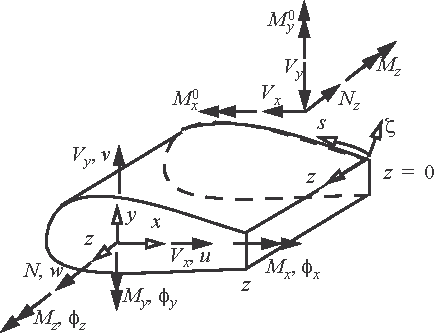
\includegraphics{Figure_8-4.pdf}}{\caption{Closed cross-sectional bar   subject to free bending and torsion.}\label{fig8.4}}

\vspace*{-30pt}

\begin{align}\label{eq8.38}
\frac{d N}{d z}=0 \quad \frac{d V_{x}}{d z}=0 \quad \frac{d
V_{y}}{d z}=0 \quad \frac{d M_{z}}{d z}=0 \quad 0 \leq z \leq L.
\end{align}

\pagebreak

\noindent Hence, the axial force $N$, shear forces $V_x$ and $V_y$, and the
torque $M_z$ are uniform along the length $L$ of the bar. Bending
moment equilibrium equations (\ref{eq3.55}) and (\ref{eq3.57}) on
page \pageref{eq3.57} are satisfied by
\begin{align}\label{eq8.39}
M_{x}=M_{x}^{0}+V_{y} z \quad M_{y}=M_{y}^{0}+V_{x} z \quad 0 \leq
z \leq L,
\end{align}
where $M_{x}^{0}$ and $M_{y}^{0}$ are the bending moments acting
on the cross section at $z=0$.

Consider a free body diagram of the stress resultants acting on a
segment of the wall with dimensions $\Delta s$-by-$\Delta z$ is
shown in figure~\ref{fig8.5}.

\processfigure{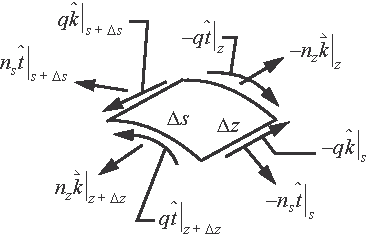
\includegraphics{Figure_8-5.pdf}}{\caption{Stress resultants acting on an element of the wall.}\label{fig8.5}}

\noindent Force equilibrium leads to
\begin{align}\label{eq8.40}
\left[\left.n_{z} \Delta s \harp{k}\right|_{z+\Delta z}-\left.n_{z}
\Delta s \harp{k}\right|_{z}\right]+\left[\left.q \Delta z
\hat{k}\right|_{s+\Delta s}-\left.q \Delta z
\hat{k}\right|_{s}\right]+\left[\left.q \Delta s
\hat{t}\right|_{z+\Delta z}-\left.q \Delta s
\hat{t}\right|_{z}\right]+\left[\left.n_{s} \Delta z
\hat{t}\right|_{s+\Delta s}-\left.n_{s} \Delta z
\hat{t}\right|_{s}\right]=0.
\end{align}
Expand the functions $n(s,z)$, $q(s,z)$, and $n_s(s,z)$ in a
Taylor series about $s$ and $z$ to get
\begin{align}
&\left(n_{z}+\frac{\partial n_{z}}{\partial z} \Delta
z-n_{z}\right) \Delta s \hat{k}+\left(q+\frac{\partial q}{\partial
s} \Delta s-q\right) \Delta z \hat{k} \nonumber\\
&\hspace*{-3pt}\qquad+\left(q+\frac{\partial
q}{\partial z} \Delta z-q\right) \Delta s \hat{t}+\left(n_{s}
\hat{t}+\frac{\partial n_{s} \hat{t}}{\partial s} \Delta s-n_{s}
\hat{t}\right) \Delta z+O\left(\Delta s^{2}, \Delta
z^{2}\right)=0. \label{eq8.41}
\end{align}
Division of eq.~(\ref{eq8.41}) by the product $\Delta s \cdot
\Delta z$, followed by taking the limit as $\Delta s \rightarrow
0$ and $\Delta z \rightarrow 0$ leads to the differential
equations
\begin{align*}
\left(\frac{\partial n_{z}}{\partial z}+\frac{\partial q}{\partial
s}\right) \hat{k}+\left(\frac{\partial q}{\partial
z}+\frac{\partial n_{s}}{\partial s}\right) \hat{t}+n_{s}
\frac{\partial \hat{t}}{\partial s}=0.
\end{align*}
From eq.~(\ref{eq3.6}) on page \pageref{eq3.6} the derivative of the unit
tangent vector is $\frac{\partial \hat{t}}{\partial
s}=\frac{-\hat{n}}{R_{s}}$, where $R_s$ is the radius of curvature
of the contour. The differential equations of equilibrium at
coordinates $s$ and $z$ in the wall are
\begin{align}\label{eq8.42}
\frac{\partial n_{z}}{\partial z}+\frac{\partial q}{\partial s}=0
\quad \frac{\partial q}{\partial z}+\frac{\partial n_{s}}{\partial
s}=0 \quad \frac{-n_{s}}{R_{s}}=0.
\end{align}
From the last two equations in (\ref{eq8.42}) we get
\begin{align}\label{eq8.43}
n_{s}=0 \quad \frac{\partial q}{\partial z}=0.
\end{align}
That is, the circumferential stress resultant vanishes and the
shear flow is independent of the longitudinal coordinate~$z$.

\subsection{Anisotropic Hooke's law for the cross section}\label{sec8.2.1}

Set $n_{s}=0$ in eq.~(\ref{eq8.35}), and solve for the normal
strain $\varepsilon_{ss}$ to eliminate it in the material law. We
write the resulting material law in several forms to be used in
subsequent developments:
\begin{gather}
n_{z}=B \varepsilon_{z z}+b q \quad q=B_{s} \gamma_{s z}+B_{z}
\varepsilon_{z z}\mbox{, and}\label{eq8.44}\\
\varepsilon_{z z}=\frac{1}{B}\left(n_{z}-b q\right) \quad
\gamma_{s z}=\frac{1}{B}\left(a q-b n_{z}\right).\label{eq8.45}
\end{gather}
The coefficients in the previous equations are
\begin{gather}
B=A_{22}-A_{12} A_{21}/ A_{11}-b B_{z},\label{eq8.46}\\
B_{s}=A_{66}-A_{61} A_{16}/ A_{11} \quad B_{z}=A_{62}-A_{12}
A_{61}/ A_{11}\mbox{, and}\label{eq8.47}\\
a=\frac{1}{B_{s}}\left(A_{22}-A_{12} A_{21}/ A_{11}\right) \quad
b=B_{z}/ B_{s}.\label{eq8.48}
\end{gather}
The stiffness parameters $b$ and $B_{z}$ represent the
shear-extension coupling of the laminated wall, since they are
directly related to stiffnesses $A_{61}$ and $A_{62}$ by eqs.
(\ref{eq8.47}) and (\ref{eq8.48}). In a specially orthotropic
laminate $A_{61}={A_{62}=0}$, so $b={B_{z}=0}$. There is no material
coupling between shear and extension in a specially orthotropic
laminate.

The second assumption is traditional for the beam theory and
states that the axial strain is a linear function of coordinates
$x$ and $y$. From eq.~(\ref{eq3.30}) on page \pageref{eq3.30} the axial normal
strain along the contour ($\zeta=0$) is
\begin{align}\label{eq8.49}
\varepsilon_{z z}=\frac{d w}{d z}+y(s) \frac{d \phi_{x}}{d z}+x(s)
\frac{d \phi_{y}}{d z}.
\end{align}
where $w(z)$ is the axial displacement of the cross section,
$\phi_{x}(z)$ is the rotation of the cross section about the
$x$-axis, and $\phi_{y}(z)$ is the rotation of the cross section
about the negative $y$-axis. Refer to figure~\ref{fig8.4}.
Substitute eq.~(\ref{eq8.49}) for the strain in the first equation
of (\ref{eq8.44}) to get the normal stress resultant as
\begin{align}\label{eq8.50}
n_{z}=B\left(\frac{d w}{d z}+y(s) \frac{d \phi_{x}}{d z}+x(s)
\frac{d \phi_{y}}{d z}\right)+b q.
\end{align}
Substitute the previous expression for the normal stress resultant
into the definition of the bar resultant $N$ in eq.~(\ref{eq3.39})
on page \pageref{eq3.39} to get
\begin{align}\label{eq8.51}
N=\oint n_{z} d s=S\left(\frac{d w}{d z}\right)+S_{x}\left(\frac{d
\phi_{x}}{d z}\right)+S_{y}\left(\frac{d \phi_{y}}{d
z}\right)+\oint(b q) d s,
\end{align}
where
\begin{align}\label{eq8.52}
S=\oint B(s) d s \quad S_{x}=\oint B(s) y(s) d s \quad S_{y}=\oint
B(s) x(s) d s.
\end{align}
In eq.~(\ref{eq8.52}) the modulus-weighted extensional stiffness
of the cross section of the beam is denoted by $S$, the
modulus-weighted first moment of the cross-sectional area about
the $x$-axis by $S_{x}$, and the modulus-weighted first moment of
the cross-sectional area about the $y$-axis by $S_{y}$. We now
locate the origin of the \textit{x-y} coordinates at the
modulus-weighted centroid of the cross section. Let
$x(s)=X(s)-X_{c}$ and $y(s)=Y(s)-Y_{c}$, where $X(s)$ and $Y(s)$
are the Cartesian coordinates of the contour with respect to an
arbitrary origin at point $O$ (see Fig.~\ref{fig3.1} on page
\pageref{fig3.1}). The coordinates ($X_c,Y_c$) of the
modulus-weighted centroid are determined from
\begin{align}\label{eq8.53}
S_{x}=0=\oint B(s) Y(s) d s-Y_{c} S \quad S_{y}=0=\oint B(s) X(s)
d s-X_{c} S.
\end{align}
Since $S_{x}=S_{y}=0$, eq.~(\ref{eq8.51}) is written as
\begin{align}\label{eq8.54}
\bar{N}=S\left(\frac{d w}{d z}\right) \quad \text { where } \quad
\bar{N}=N-\oint(b q) d s.
\end{align}
The bending moments $M_x$ and $M_y$ acting in the cross section
are determined from the normal stress resultant $n_{z}$ by
\begin{align}\label{eq8.55}
M_{x}=\oint\left(y n_{z}\right) d s \quad M_{y}=\oint\left(x
n_{z}\right) d s.
\end{align}
Substitute eq.~(\ref{eq8.50}) for the normal stress resultant into
these expressions for the bending moments to get
\begin{align}\label{eq8.56}
M_{x}=D_{x x}\left(\frac{d \phi_{x}}{d z}\right)+D_{x
y}\left(\frac{d \phi_{y}}{d z}\right)+\oint(y b q) d s \quad
M_{y}=D_{x y}\left(\frac{d \phi_{x}}{d z}\right)+D_{y
y}\left(\frac{d \phi_{y}}{d z}\right)+\oint(x b q) d s.
\end{align}
The modulus-weighted second moments of the cross section appearing
in eq.~(\ref{eq8.56}) are defined by
\begin{align}\label{eq8.57}
\left[\begin{array}{@{}lll@{}}D_{x x} & D_{y y} & D_{x
y}\end{array}\right]=\oint\left[\begin{array}{@{}lll@{}}y^{2} & x^{2} &
x y\end{array}\right] B d s.
\end{align}
Solve for the gradients of the bending rotations
eq.~(\ref{eq8.56}) and write the result as
\begin{align}\label{eq8.58}
\left[\begin{array}{@{}c@{}}\frac{d \phi_{x}}{d z}\\
[6pt]
\frac{d
\phi_{y}}{d
z}\end{array}\right]=k\left[\begin{array}{@{}cc@{}}\frac{1}{D_{x
x}} & \frac{-n_{x}}{D_{y y}}\\
[6pt]
\frac{-n_{y}}{D_{x x}} &
\frac{1}{D_{y
y}}\end{array}\right]\left[\begin{array}{@{}l@{}}\bar{M}_{x}\\
\bar{M}_{y}\end{array}\right],
\end{align}
where
\begin{align}\label{eq8.59}
n_{x}=\frac{D_{x y}}{D_{x x}} \quad n_{y}=\frac{D_{x y}}{D_{y y}}
\quad k=\frac{1}{1-n_{x} n_{y}},
\end{align}
and
\begin{align}\label{eq8.60}
\bar{M}_{x}=M_{x}-\oint(y b q) d s \quad \bar{M}_{y}=M_{y}-\oint(x
b q) d s.
\end{align}
Substitute eq.~(\ref{eq8.54}) for the axial displacement gradient,
and eq.~(\ref{eq8.58}) for the bending rotation gradients, into
eq.~(\ref{eq8.50}) to express the normal stress resultant as
\begin{align}\label{eq8.61}
n_{z}=\frac{B}{S} \bar{N}+B \bar{y}(s) \frac{k}{D_{x x}}
\bar{M}_{x}+B \bar{x}(s) \frac{k}{D_{y y}} \bar{M}_{y}+b q,
\end{align}
where
\begin{align}\label{eq8.62}
\bar{x}(s)=x(s)-n_{x} y(s) \quad \bar{y}(s)=y(s)-n_{y} x(s).
\end{align}

\subsection{Expressions for the shear flow and normal stress resultant}\label{sec8.2.2}

Substitute the normal stress resultant from eq.~(\ref{eq8.61})
into the equilibrium differential equation (\ref{eq8.42}), to get
\begin{align}\label{eq8.63}
\frac{d q}{d s}=-\left(\frac{B}{S}\right) \frac{d \bar{N}}{d z}-B
\bar{y} \frac{k}{D_{x x}} \frac{d \bar{M}_{x}}{d z}-B \bar{x}
\frac{k}{D_{y y}} \frac{d \bar{M}_{y}}{d z}.
\end{align}
\vspace*{2pt}
\clearpage

\noindent Recall that the stiffness parameter $b$ and the shear flow $q$ are
independent of coordinate $z$. Derivatives of $\bar{N}$,
$\bar{M}_{x}$, and $\bar{M}_{y}$ with respect to $z$ are
determined from eqs. (\ref{eq8.54}) and (\ref{eq8.60}) as
\begin{align}\label{eq8.64}
\frac{d \bar{N}}{d z}=\frac{d N}{d z} \quad \frac{d \bar{M}_{x}}{d
z}=\frac{d M_{x}}{d z} \quad \frac{d \bar{M}_{y}}{d z}=\frac{d
M_{y}}{d z}.
\end{align}
Derivatives of the bar resultants are given by equilibrium
equations (\ref{eq8.38}) and (\ref{eq8.39}). Thus,
\begin{align}\label{eq8.65}
\frac{d N}{d z}=0 \quad \frac{d M_{x}}{d z}=V_{y} \quad \frac{d
M_{y}}{d z}=V_{x}.
\end{align}
The derivative of the shear flow with respect to the contour
coordinate reduces to
\begin{align}\label{eq8.66}
\frac{d q}{d s}=-B \bar{y} \frac{k}{D_{x x}} V_{y}-B \bar{x}
\frac{k}{D_{y y}} V_{x}.
\end{align}
Now we integrate the previous result with respect to the contour
coordinate from $s = 0$ to $s = s$ and write the result as
\begin{align}\label{eq8.67}
q(s)=q_{0}-\bar{S}_{x}(s) \frac{k}{D_{x x}} V_{y}-\bar{S}_{y}(s)
\frac{k}{D_{y y}} V_{x},
\end{align}
where
\begin{align}\label{eq8.68}
q_{0}=q(0) \quad \bar{S}_{x}(s)=\int_{0}^{s} B \bar{y}(s) d s
\quad \bar{S}_{y}(s)=\int_{0}^{s} B \bar{x}(s) d s.
\end{align}
Substitute eq.~(\ref{eq8.62}) for $\bar{x}(s)$ and $\bar{y}(s)$
into eq.~(\ref{eq8.68}) to get
\begin{align}\label{eq8.69}
\bar{S}_{x}(s)=S_{x}(s)-n_{y} S_{y}(s) \quad
\bar{S}_{y}(s)=S_{y}(s)-n_{x} S_{x}(s),
\end{align}
where the modulus-weighted first moments of a segment of the
cross-sectional area from $s = 0$ to $s = s$ are defined by
\begin{align}\label{eq8.70}
S_{x}(s)=\int_{0}^{s} B(s) y(s) d s \quad S_{y}(s)=\int_{0}^{s}
B(s) x(s) d s.
\end{align}
Note that $S_{x}(s)$ and $S_{y}(s)$ evaluated at the end point of
the closed contour vanish, which is consistent with
eq.~(\ref{eq8.53}). The shear flow at the contour origin $q_0$ is
determined by torque equivalence of the shear flow with respect to
the modulus-weighted centroid. That is,
\begin{align}\label{eq8.71}
M_{z c}=\oint r_{n c}(s) q(s) d s,
\end{align}
where $r_{n c}(s)$ is the coordinate normal to the contour as
depicted in Fig.~\ref{fig3.3} on page \pageref{fig3.3}, and it is
determined from eq.~(\ref{eq3.11}) on page \pageref{eq3.11}.
Substitute eq.~(\ref{eq8.67}) for the shear flow in
eq.~(\ref{eq8.71}) and solve for $q_0$ to find
\begin{align}\label{eq8.72}
q_{0}=\frac{1}{2 A_{c}}\left[M_{z c}+\left(\frac{k V_{y}}{D_{x
x}}\right) \oint\left(r_{n c} \bar{S}_{x}\right) d s+\left(\frac{k
V_{x}}{D_{y y}}\right) \oint\left(r_{n c} \bar{S}_{y}\right) d
s\right],
\end{align}
where the area enclosed by the contour is given by
\begin{align}\label{eq8.73}
A_{c}=\frac{1}{2} \oint r_{n c} d s.
\end{align}
With $q_0$ determined, we write the final expression for the shear
flow in eq.~(\ref{eq8.67}) as
\begin{align}\label{eq8.74}
\fbox{$\displaystyle q(s)=\frac{M_{z c}}{2 A_{c}}-F_{x c}(s)
V_{x}-F_{y c}(s) V_{y},$}
\end{align}
where the shear flow distribution functions are defined by
\begin{align}\label{eq8.75}
F_{x c}(s)=\frac{k}{D_{y y}}\left[\overline{S_{y}}(s)-\frac{1}{2
A_{c}} \oint\left(r_{n c} \bar{S}_{y}\right) d s\right] \quad F_{y
c}(s)=\frac{k}{D_{x x}}\left[\bar{S}_{x}(s)-\frac{1}{2 A_{c}}
\oint\left(r_{n c} \bar{S}_{x}\right) d s\right].
\end{align}

\removelastskip

Substitute eq.~(\ref{eq8.54}) for the normal stress resultant
$\bar{N}$ in eq.~(\ref{eq8.61}), and substitute for $\bar{M}_{x}$
and $\bar{M}_{y}$ from eq.~(\ref{eq8.60}) into eq.~(\ref{eq8.61}),
to get
\begin{align}\label{eq8.76}
n_{z}=\frac{B}{S}[N-\oint(b q) d s]+B \bar{y} \frac{k}{D_{x
x}}\left[M_{x}-\oint(y b q) d s\right]+B \bar{x} \frac{k}{D_{y
y}}\left[M_{y}-\oint(x b q) d s\right]+b q.
\end{align}
Substitute eq.~(\ref{eq8.74}) for the shear flow into the previous
equation for the normal stress resultant. After some algebraic
manipulations we write the result as
\begin{align}\label{eq8.77}
\fbox{$\displaystyle n_{z}=\frac{B}{S} N+B \bar{y}(s)
\frac{k}{D_{x x}} M_{x}+B \bar{x}(s) \frac{k}{D_{y y}}
M_{y}+\Phi_{x}(s) V_{x}+\Phi_{y}(s) V_{y}+\Phi(s) \frac{M_{z c}}{2
A_{c}}.$}
\end{align}
The functions $\Phi_{x}(s)$, $\Phi_{y}(s)$, and $\Phi(s)$ are a
consequence of the coupling between extension and shear in the
material law (i.e., $b \neq 0$). If the stiffness parameter $b=0$
over the entire contour, then $\Phi_{x}(s)=\Phi_{y}(s)=\Phi(s)=0$.
Equations for these functions are
\begin{gather}
\Phi_{x}(s)=-b F_{x c}(s)+\frac{B}{S}\left(\oint b F_{x c} d
s\right)+\frac{B k \bar{y}(s)}{D_{x x}}\left(\oint b y F_{x c} d
s\right)+\frac{B k \bar{x}(s)}{D_{y y}}\left(\oint b x F_{x c} d
s\right),\label{eq8.78}\\
\Phi_{y}(s)=-b F_{y c}(s)+\frac{B}{S}\left(\oint b F_{y c} d
s\right)+\frac{B k \bar{y}(s)}{D_{x x}}\left(\oint b y F_{y c} d
s\right)+\frac{B k \bar{x}(s)}{D_{y y}}\left(\oint b x F_{y c} d
s\right)\mbox{, and }\label{eq8.79}\\
\Phi(s)=b-\frac{B}{S} \oint b d s-\frac{B k \bar{y}(s)}{D_{x x}}
\oint b y d s-\frac{B k \bar{x}(s)}{D_{y y}} \oint b x d
s.\label{eq8.80}
\end{gather}

\subsection{Complementary work and energy}\label{sec8.2.3}

Consider a free bending and torsion state of the bar as shown in
figure~\ref{fig8.4} where the displacements, strains, and forces satisfy
the compatibility conditions, Hooke's law, and the equilibrium
conditions. In this state, the actual displacements of the
modulus-weighted centroid are $u_{c}(z)$, $v_{c}(z)$, and $w(z)$,
and the corresponding forces are $V_{x}(z)$, $V_{y}(z)$, and
$N(z)$, respectively. The actual rotations of a cross section with
respect to the modulus-weighted centroid are $\phi_{x}(z),
\phi_{y}(z)$, and $\phi_{z}(z)$, and the corresponding moments are
$M_{x}(z), M_{y}(z)$, and $M_{z c}(z)$, respectively. Now consider
infinitesimal increments in the forces and moments denoted by
$\delta V_{x}, \delta V_{y}, \delta N, \delta M_{x},\delta M_{y}$,
and $\delta M_{z C}$ from the equilibrium state. For an element of
the bar of length $\Delta z$, the complementary work is given by
\begin{align}\label{eq8.81}
\delta \bar{U}^{*} \Delta z=\left.\left[\delta V_{x} u_{c}+\delta
V_{y} v_{c}+\delta N w+\delta M_{x} \phi_{x}+\delta M_{y}
\phi_{y}+\delta M_{z c} \phi_{z}\right]\right|_{z} ^{z+\Delta z},
\end{align}
where $\delta \bar{U}^{*}$ denotes the increment in the
complementary work per unit axial length. Divide
eq.~(\ref{eq8.81}) by $\Delta z$, and let $\Delta z \rightarrow
0$, to get in the limit
\begin{align}\label{eq8.82}
\delta \bar{U}^{*}=\frac{d}{d z}\left[\delta V_{x} u_{c}+\delta
V_{y} v_{c}+\delta N w+\delta M_{x} \phi_{x}+\delta M_{y}
\phi_{y}+\delta M_{z C} \phi_{z}\right].
\end{align}
\vspace*{2pt}\vspace*{-10pt}
\clearpage

\noindent Statically admissible incremental actions requires that they
satisfy the equilibrium differential equations (\ref{eq8.38}) and
(\ref{eq8.39}): i.e.,
\begin{align}\label{eq8.83}
\frac{d}{d z} \delta V_{x}=\frac{d}{d z} \delta V_{y}=\frac{d}{d
z} \delta N=\frac{d}{d z} \delta M_{z c}=0 \qquad \frac{d}{d z}
\delta M_{x}=\delta V_{y} \quad \frac{d}{d z} \delta M_{y}=\delta
V_{x}.
\end{align}
Imposing equilibrium (\ref{eq8.83}) reduces eq.~(\ref{eq8.82}) to
\begin{align}\label{eq8.84}
\delta \bar{U}^{*}=\psi_{x c} \delta V_{x}+\psi_{y c} \delta
V_{y}+\left(\frac{d w}{d z}\right) \delta N+\left(\frac{d
\phi_{x}}{d z}\right) \delta M_{x}+\left(\frac{d \phi_{y}}{d
z}\right) \delta M_{y}+\left(\frac{d \phi_{z}}{d z}\right) \delta
M_{z} c,
\end{align}
where shear strains averaged over the cross section of the bar
relative to the centroid are defined by
\begin{align}\label{eq8.85}
\psi_{x c}=\frac{d u_{c}}{d z}+\phi_{y} \quad \psi_{y c}=\frac{d
v_{c}}{d z}+\phi_{x}.
\end{align}
An elastic material is defined by the existence of a complementary
strain energy function per unit axial length with the form
$\bar{U}^{*}\left(M_{x}, M_{y}, N, V_{x}, V_{y}, M_{z C}\right)$.
Then, the total increment in function $\bar{U}^{*}$ is
\begin{align}\label{eq8.86}
\delta \bar{U}^{*}=\frac{\partial \bar{U}^{*}}{\partial M_{x}}
\delta M_{x}+\frac{\partial \bar{U}^{*}}{\partial M_{y}} \delta
M_{y}+\frac{\partial \bar{U}^{*}}{\partial N} \delta
N+\frac{\partial \bar{U}^{*}}{\partial V_{x}} \delta
V_{x}+\frac{\partial \bar{U}^{*}}{\partial V_{y}} \delta
V_{y}+\frac{\partial \bar{U}^{*}}{\partial M_{zC} } \delta M_{zC},
\end{align}
Identify the complementary work (\ref{eq8.84}) with the
complementary energy (\ref{eq8.86}) to get the important
properties of complementary strain energy function. That is,
\begin{align}\label{eq8.87}
\frac{d \phi_{x}}{d z}=\frac{\partial \bar{U}^{*}}{\partial M_{x}}
\quad \frac{d \phi_{y}}{d z}=\frac{\partial \bar{U}^{*}}{\partial
M_{y}} \quad \frac{d w}{d z}=\frac{\partial \bar{U}^{*}}{\partial
N} \quad \psi_{x c}=\frac{\partial \bar{U}^{*}}{\partial V_{x}}
\quad \psi_{y c}=\frac{\partial \bar{U}^{*}}{\partial V_{y}} \quad
\frac{d \phi_{z}}{d z}=\frac{\partial \bar{U}^{*}}{\partial M_{z
C}}.
\end{align}

\vspace*{-1pc}

Now consider the complementary work for the free bending and
torsion state of an element of the wall $\Delta s$-by-$\Delta z$
as shown in Fig.~\ref{fig8.5}. On the contour ($\zeta=0$) the
axial displacement $u_{z}(s, z)$ corresponds to the stress
resultant $n_z$ and tangential displacement $u_{s}(s, z)$
corresponds to the shear flow $q$. Let $\delta U_{o}^{*}$ denote
the increment in the complementary work per unit area for
increments in the stress resultants $\delta n_z$ and $\delta q$
acting on the element $\Delta s$-by-$\Delta z$ of
Fig.~\ref{fig8.5}. Then, the complementary work is
\begin{align}\label{eq8.88}
\delta U_{o}^{*} \Delta s \Delta z=\left.\left[\left(\delta n_{z}
\Delta s\right) u_{z}+(\delta q \Delta s) u_{s}\right]\right|_{z}
^{z+\Delta z}+\left.\left[(\delta q \Delta z)
u_{z}\right]\right|_{s s} ^{s+\Delta s}.
\end{align}
Divide eq.~(\ref{eq8.88}) by $\Delta s \Delta z$, and let $\Delta
s \rightarrow 0$ and $\Delta z \rightarrow 0$, to get in the limit
\begin{align}\label{eq8.89}
\delta U_{0}^{*}=\frac{\partial}{\partial z}\left[\left(\delta
n_{z}\right) u_{z}+(\delta q)
u_{s}\right]+\frac{\partial}{\partial s}\left[(\delta q)
u_{z}\right],
\end{align}
which expands to
\begin{align}\label{eq8.90}
\delta U_{o}^{*}=\left[\frac{\partial}{\partial z}\left(\delta
n_{z}\right)+\frac{\partial}{\partial s}(\delta q)\right]
u_{z}+\left[\frac{\partial}{\partial z}(\delta q)\right]
u_{s}+\frac{\partial u_{z}}{\partial z} \delta
n_{z}+\left(\frac{\partial u_{z}}{\partial s}+\frac{\partial
u_{s}}{\partial z}\right) \delta q.
\end{align}
Statically admissible increments in the stress resultants $\delta
n_z$ and $\delta q$ requires that they satisfy equilibrium
equations (\ref{eq8.42}) and (\ref{eq8.43}), which are
\begin{align}\label{eq8.91}
\frac{\partial}{\partial z}\left(\delta
n_{z}\right)+\frac{\partial}{\partial s}(\delta q)=0 \quad
\frac{\partial}{\partial z}(\delta q)=0.
\end{align}
From the strain-displacement relations (\ref{eq3.27}) and
(\ref{eq3.28}) on page \pageref{eq3.28} we identify the axial
normal strain $\varepsilon_{z z}$ and the shear strain $\gamma_{s
z}$ as
\begin{align}\label{eq8.92}
\varepsilon_{z z}=\frac{\partial u_{z}}{\partial z} \quad
\gamma_{s z}=\frac{\partial u_{z}}{\partial s}+\frac{\partial
u_{s}}{\partial z}.
\end{align}
Substitute eqs. (\ref{eq8.91}) and (\ref{eq8.92}) into
eq.~(\ref{eq8.90}) to get the increment in the complementary work
per unit area as
\begin{align}\label{eq8.93}
\delta U_{o}^{*}=\varepsilon_{z z} \delta n_{z}+\gamma_{s z}
\delta q.
\end{align}
For an elastic material we identify $\delta U_{o}^{*}$ with the
increment in the complementary strain energy function per unit
area, which is a function of the stress resultants, or
$U_{o}^{*}\left(\dot{n}_{z}, q\right)$, with the properties
\begin{align}\label{eq8.94}
\varepsilon_{z z}=\frac{\partial U_{o}^{*}}{\partial n_{z}} \quad
\gamma_{s z}=\frac{\partial U_{o}^{*}}{\partial q}.
\end{align}
Now substitute Hooke's law (\ref{eq8.45}) for the normal strain
$\varepsilon_{z z}$ and for the shear strain $\gamma_{s z}$ in the
previous equation to get
\begin{align}\label{eq8.95}
\frac{\partial U_{o}^{*}}{\partial n_{z}}=\frac{1}{B}\left(n_{z}-b
q\right) \quad \frac{\partial U_{o}^{*}}{\partial
q}=\frac{1}{B}\left(a q-b n_{z}\right).
\end{align}
The complementary strain energy function per unit area consistent
with these properties (\ref{eq8.95}) is
\begin{align}\label{eq8.96}
U_{o}^{*}=\frac{1}{2 B}(n_{z}^{2}-2 b n_{z} q+a q^{2}).
\end{align}
The increment in the complementary energy per unit axial length
$\delta \bar{U}^{*}$ is defined $\delta \bar{U}^{*}=\oint \delta
U_{o}^{*} d s$. Hence,
\begin{align}\label{eq8.97}
\bar{U}^{*}=\frac{1}{2} \oint \frac{1}{B}(n_{z}^{2}-2 b n_{z}
q+a q^{2}) d s.
\end{align}
Equations (\ref{eq8.74}) and (\ref{eq8.77}) relate the shear flow
and normal stress resultant to the bar forces $N, V_{x}$, and
$V_{y}$ and the moments $M_{x}, M_{y}$, and $M_{z}$. Imposing the
properties of the complementary strain energy for the bar given by
(\ref{eq8.87}) to the expression (\ref{eq8.97}) for the
complementary strain energy, we get the following relations:
\begin{gather}
\frac{d \phi_{x}}{d z}=\oint_{B} \frac{1}{B}\left[\left(n_{z}-b
q\right) \frac{\partial n_{z}}{\partial M_{x}}+\left(a q-b
n_{z}\right) \frac{\partial q}{\partial M_{x}}\right] d
s\label{eq8.98}\\
\frac{d \phi_{y}}{d z}=\oint \frac{1}{B}\left[\left(n_{z}-b
q\right) \frac{\partial n_{z}}{\partial M_{y}}+\left(a q-b
n_{z}\right) \frac{\partial q}{\partial M_{y}}\right] d
s\label{eq8.99}\\
\frac{d w}{d z}=\oint \frac{1}{B}\left[\left(n_{z}-b q\right)
\frac{\partial n_{z}}{\partial N}+\left(a q-b n_{z}\right)
\frac{\partial q}{\partial N}\right] d s\label{eq8.100}\\
\psi_{x c}=\oint \frac{1}{B}\left[\left(n_{z}-b q\right)
\frac{\partial n_{z}}{\partial V_{x}}+\left(a q-b n_{z}\right)
\frac{\partial q}{\partial V_{x}}\right] d s\label{eq8.101}\\
\psi_{y c}=\oint \frac{1}{B}\left[\left(n_{z}-b q\right)
\frac{\partial n_{z}}{\partial V_{y}}+\left(a q-b n_{z}\right)
\frac{\partial q}{\partial V_{y}}\right] d s\label{eq8.102}\\
\frac{d \phi_{z}}{d z}=\oint \frac{1}{B}\left[\left(n_{z}-b
q\right) \frac{\partial n_{z}}{\partial M_{z C}}+\left(a q-b
n_{z}\right) \frac{\partial q}{\partial M_{z C}}\right] d
s.\label{eq8.103}
\end{gather}
Equations (\ref{eq8.98}) to (\ref{eq8.103}) are statements of
Castigilano's second theorem.

\vspace*{8pt}

\clearpage

\subsection{Cross-sectional compliance matrix}\label{sec8.2.4}

Substitute eq.~(\ref{eq8.74}) for the shear flow, and substitute
eq.~(\ref{eq8.77}) for the normal stress resultant, into eqs.
(\ref{eq8.98}) to (\ref{eq8.103}), followed by integration over
the contour. The result from the integration leads to compliance
form of the material law:\vspace*{-9pt}\enlargethispage{1\baselineskip}
\begin{align}\label{eq8.104}
\left[\begin{array}{@{}c@{}}d \phi_{x}/ d z\\
d \phi_{y}/ d z\\
d w/ d z\\
\psi_{x c}\\
\psi_{y c}\\
d \phi_{z}/ d
z\end{array}\right]=\left[\begin{array}{@{}llllll@{}}c_{11} &
c_{12} & c_{13} & c_{14} & c_{15} & c_{16}\\
c_{21} & c_{22} &
c_{23} & c_{24} & c_{25} & c_{26}\\
c_{31} & c_{32} & c_{33} &
c_{34} & c_{35} & c_{36}\\
c_{41} & c_{42} & c_{43} & c_{44} &
c_{45} & c_{46}\\
c_{51} & c_{52} & c_{53} & c_{54} & c_{55} &
c_{56}\\
c_{61} & c_{62} & c_{63} & c_{64} & c_{65} &
c_{66}\end{array}\right]\left[\begin{array}{@{}c@{}}M_{x}\\
M_{y}\\
N\\
V_{x}\\
V_{y}\\
M_{z C}\end{array}\right].
\end{align}
Elements of the compliance matrix are given below.\vspace*{-3pt}
\begin{gather}
c_{11}=\frac{k}{D_{x x}} \quad c_{21}=\frac{-k n_{y}}{D_{x
x}}=c_{12}=\frac{-k n_{x}}{D_{y y}} \quad c_{13}=c_{31}=0 \quad
c_{14}=c_{41}=\left(\frac{k}{D_{x x}}\right) \oint\left(b \bar{y}
F_{x c}\right) d s\label{eq8.105}\\[-1pt]
c_{15}=c_{51}=\left(\frac{k}{D_{x x}}\right) \oint\left(b \bar{y}
F_{y c}\right) d s \quad c_{16}=c_{61}=\left(\frac{-k}{2 A_{c}
D_{x x}}\right) \oint(b \bar{y}) d s\label{eq8.106}\\[-1pt]
c_{22}=\frac{k}{D_{y y}} \quad c_{23}=c_{32}=0 \quad
c_{24}=c_{42}=\left(\frac{k}{D_{y y}}\right) \oint\left(b \bar{x}
F_{x c}\right) d s\label{eq8.107}\\[-1pt]
c_{25}=c_{52}=\left(\frac{k}{D_{y y}}\right) \oint\left(b \bar{x}
F_{y c}\right) d s \quad c_{26}=c_{62}=\left(\frac{-k}{2 A_{c}
D_{y y}}\right) \oint(b \bar{x}) d s \quad c_{33}=1/
S\label{eq8.108}\\[-1pt]
c_{34}=c_{43}=\left(\frac{1}{S}\right) \oint\left(b F_{x c}\right)
d s \quad c_{35}=c_{53}=\left(\frac{1}{S}\right) \oint\left(b F_{y
c}\right) d s \quad c_{36}=c_{63}=\left(\frac{-1}{2 A_{c}
S}\right) \oint(b) d s\label{eq8.109}\\[-1pt]
c_{44}=\oint \frac{1}{B}\big(a F_{x c}^{2}+2 b F_{x c}
\Phi_{x}+\Phi_{x}^{2}\big) d s \quad c_{45}=c_{54}=\oint
\frac{1}{B}\left(a F_{x c} F_{y c}+b F_{y c} \Phi_{x}+b F_{x c}
\Phi_{y}+\Phi_{x} \Phi_{y}\right) d s\label{eq8.110}\\[-1pt]
c_{46}=c_{64}=\left(\frac{1}{2 A}\right) \oint \frac{1}{B}\left(-a
F_{x c}+b F_{x c} \Phi-b \Phi_{x}+\Phi \Phi_{x}\right) d s \quad
c_{55}=\oint \frac{1}{B}\left(a F_{y c}^{2}+2 b F_{y c}
\Phi_{y}+\Phi_{y}^{2}\right) d s\label{eq8.111}\\[-1pt]
c_{56}=c_{65}=\left(\frac{1}{2 A_{c}}\right) \oint\frac{1}{B}\left(-a
F_{y c}+b F_{y c} \Phi-b \Phi_{y}+\Phi \Phi_{y}\right) d s \quad
c_{66}=\left(\frac{1}{4 A_{c}^{2}}\right) \oint
\frac{1}{B}\left(a-2 b \Phi+\Phi^{2}\right) d s.\label{eq8.112}
\end{gather}
Matrix $[c_{i j}]$ is symmetric so that twenty-one of the
coefficients are independent. The fifteen of the off-diagonal
coefficients correspond to different types of coupling effects as
described in table \ref{tab8.3}.

%Table 8.3
\begin{table}[!h]
\vspace*{-6pt}
\processtable{Description of coupling coefficients\label{tab8.3}}{%
\begin{tabular}{@{}lP{110pt}l@{}}%
\toprule
\colhead{Coefficients} & \colhead{\textbf{Coupling effects}} &
\colhead{\textbf{Comment}}\\
\midrule
 $c_{21}$ & combined bending about\break $x$- and $y$-axes & $c_{21} = 0$ if $D_{xy}=0$\\
 $c_{31}\ \&\  c_{32}$ & bending-extension & $c_{31} =c_{32} = 0$, since origin is at modulus weighted centroid\\
 $c_{41}, c_{51}, c_{42},\ \&\ c_{52}$ & bending-shearing & are zero if parameter $b = 0$ over entire contour\\
 $c_{61}\ \&\ c_{62}$ & bending-torsion & are zero if parameter $b = 0$ over entire contour\\
 $c_{43}\ \&\ c_{53}$ & shearing-extension & are zero if parameter $b = 0$ over entire contour\\
 $c_{63}$ & torsion-extension & is zero if parameter $b = 0$ over entire contour\\
 $c_{64}\ \&\ c_{65}$ & torsion-shearing\\
 $c_{45}$ & combined transverse shear in \textit{x-z} and \textit{y-z} planes\\
\botrule%
\end{tabular}}{}
\vspace*{-8pt}
\end{table}

\begin{example}[Graphite-epoxy circular tube]\label{ex8.3}Nixon (1987) conducted experiments on thin-walled tubes fabricated
from T300/5208 graphite/epoxy. The test specimens had a mean
radius $R = 20.32$~mm, a wall thickness $t = 1.016$~mm, and were
composed of two unidrectional layers with angles
$\varphi_{1}=-20^{\circ}$ and $\varphi_{2}=70^{\circ}$. The
thickness of both layers is the same, and the properties of the
material are $E_1 = 146.7$~GPa (21.3~ksi), $E_2 = 11.0$~GPa
(1.6~ksi), $G_{12} = 6.41$~GPa (0.93~ksi), principal Poisson's
ration $v_{21}=0.38$ and the minor Poisson's ratio
$v_{12}=0.0285$. The twist per unit length $d \phi_{z}/ d z$ was
measured in the experiment for an applied axial force \textit{N}
and an applied torque $M_{z}$. Determine this relationship from
the composite bar theory.

\subsubsection{Solution.} The in-plane stiffness matrix is
determined from $[A]=\left[\bar{Q}\left(\varphi_{1}\right)\right]\!
\frac{t}{2}+\left[\bar{Q}\left(\varphi_{2}\right)\right]\!\frac{t}{2}$, where the formulas for the elements of transformed
reduced stiffness matrix are listed in eq.~(\ref{eq8.35}). The
result is
\begin{align}\label{ex5.3a}
\left[\begin{array}{@{}ccc@{}}A_{11} & A_{12} & A_{16}\\
A_{21} & A_{22} & A_{26}\\
A_{61} & A_{62} &
A_{66}\end{array}\right]=\left[\begin{array}{@{}ccc@{}}67.8649 &
17.4628 & 15.6839\\
17.4628 & 67.8649 & -15.6839\\
15.6839 &
-15.6839 & 19.6701\end{array}\right]\,\mathrm{MN}/
\mathrm{m}.\tag{a}
\end{align}
From eqs. (\ref{eq8.47}) and (\ref{eq8.48}) the stiffness
parameters of the composite bar theory are
\begin{align}\label{ex5.3b}
B_{s}=16.0454\,\mathrm{MN}/\mathrm{m} \quad B_{z}=-19.7196\,\mathrm{MN}/\mathrm{m} \quad b=-1.22899 \quad B=39.1363\,\mathrm{MN}/\mathrm{m} \quad a=3.9495.\tag{b}
\end{align}
Note that the stiffness parameters are spatially uniform over the
entire contour. Cartesian coordinates relative to the center of
the circular contour are $x=R \cos \theta$ and $y=R \sin \theta$,
$0 \leq \theta<2 \pi$. From eq.~(\ref{eq8.52}) the axial stiffness
is $S=4.99669\,\mathrm{MN}$, and the modulus-weighted first moments
(\ref{eq8.70}) are
\begin{align}\label{ex5.3c}
S_{x}=\oint B(s) y(s) d s=B \int_{0}^{2 \pi} y(\theta) R d
\theta=0 \quad S_{y}=\oint B(s) x(s) d s=B \int_{0}^{2 \pi}
x(\theta) R d \theta=0.\tag{c}
\end{align}
As a consequence of eq.~(\textbf{\ref{ex5.3c}}) the modulus-weighted
centroid coincides with the center of the circular contour. The
modulus-weighed second moments are computed from
eq.~(\ref{eq8.57}), and the results are
\begin{align}\label{ex5.3d}
D_{x x}=D_{y y}=\pi B R^{3}=1,031.57\,\textrm{N-m}^{2}
\quad D_{x y}=0.\tag{d}
\end{align}
Thus, from eq.~(\ref{eq8.59}) and eq.~(\ref{eq8.62}) we find
$n_{x}=n_{y}=0$, $k=1$, $\bar{x}=x$, and $\bar{y}=y$. The combined
first moment functions in eq.~(\ref{eq8.69}) are computed from the
first moment functions in eq.~(\ref{eq8.70}). The results are
\begin{align}\label{ex5.3e}
\bar{S}_{x}(\theta)=B R^{2}(1-\cos \theta) \quad
\bar{S}_{y}(\theta)=B R^{2} \sin \theta.\tag{e}
\end{align}
Note that $\bar{S}_{x}(0)=\bar{S}_{y}(0)=\bar{S}_{x}(2
\pi)=\bar{S}_{y}(2 \pi)=0$. The shear flow distribution functions
$F_{xc}$ and $F_{yc}$ are computed from eq.~(\ref{eq8.75}).
Functions $\Phi_{x}, \Phi_{y}, \Phi$, which couple shear and
torsion to the normal stress resultant (\ref{eq8.77}), are
computed from eqs. (\ref{eq8.78}) to (\ref{eq8.80}). In this
example, the results for these functions are
\begin{align}\label{ex5.3f}
F_{x c}=\frac{\sin \theta}{\pi R} \quad F_{y c}=\frac{-\cos
\theta}{\pi R} \quad \Phi_{x}=\Phi_{y}=\Phi=0 \quad 0 \leq
\theta<2 \pi . \tag{f}
\end{align}
\vspace*{3pt}
\pagebreak

Elements of the compliance matrix are determined by eqs.
(\ref{eq8.105}) to (\ref{eq8.112}). In this example the result for
the cross-sectional compliance matrix is
\begin{align}\label{ex5.3g}
\left[\begin{array}{@{}c@{}}
d \phi_{x}/ d z\\
[4pt]
d \phi_{y}/ d z\\
[4pt]
d w/ d z\\
[4pt]
\psi_{x}\\
[4pt]
\psi_{y}\\
[4pt]
d \phi_{z}/ dz
\end{array}\right]=\frac{1}{\pi B
R^{3}}\left[\begin{array}{@{}cccccc@{}}1 & 0 & 0 & b R & 0 & 0\\
0
& 1 & 0 & 0 & -b R & 0\\
0 & 0 & \frac{R^{2}}{2} & 0 & 0 &
\frac{-b R}{2}\\
b R & 0 & 0 & a R^{2} & 0 & 0\\
0 & -b R & 0 & 0
& a R^{2} & 0\\
0 & 0 & \frac{-b R}{2} & 0 & 0 &
\frac{a}{2}\end{array}\right]\left[\begin{array}{@{}c@{}}M_{x}\\
M_{y}\\
N\\
V_{x}\\
V_{y}\\
M_{z}\end{array}\right].\tag{g}
\end{align}

The twist per unit length, or unit twist, for the circular tube is
equal to $c_{63} N+c_{66} M_{z}$. The unit twist evaluates as
\begin{align}\label{ex5.3h}
\frac{d \phi_{z}}{d z}=\left(\frac{-b}{2 \pi B R^{2}}\right)
N+\left(\frac{a}{2 \pi B R^{3}}\right) M_{z}=(1.21043 \times
10^{5}) N+(1.91431 \times 10^{-3})
M_{z}.\tag{h}
\end{align}
The unit twist in eq. (\textbf{\ref{ex5.3h}}) is plotted with respect to
the torque in figure~\ref{fig8.6} for two values of the axial
force. Discrete measurements from the experiment reported by Nixon
(1987) are shown by filled circles in the plot.
\end{example}

\processfigure{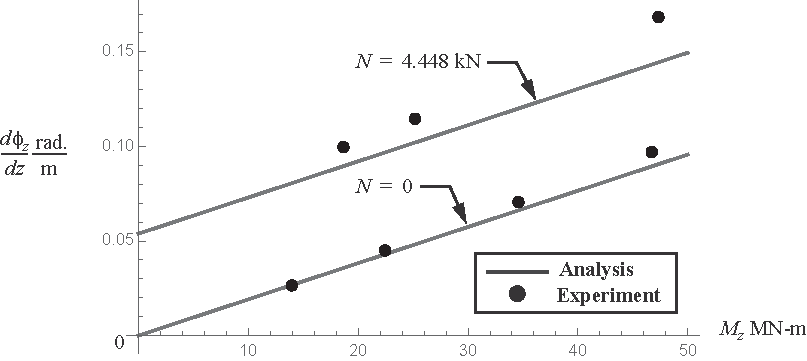
\includegraphics{Figure_8-6.pdf}}{\caption{Example 8.3: Unit twist versus torque for the two values of the axial force.}\label{fig8.6}}



\begin{example*}[Composite box beam]\label{ex8.4}Consider the composite box beam in the experiments conducted by
Smith and Chopra (1991) and Chandra et al. (1990). As shown in
figure~\ref{fig8.7}, the beam is clamped at its left end where the
axial coordinate $z=0$, $0 \leq z \leq L$, where the length of the
beam $L = 762$~mm. The cross-sectional dimensions of the
rectangular contour are $b_{x}=24.2\,\mathrm{mm}$ and
$b_{y}=13.6\,\mathrm{mm}$, and the wall thickness
$t=0.76\,\mathrm{mm}$ over the entire contour. The material is
unidirectional tape of carbon-epoxy with properties
$E_{1}=142\,\mathrm{GPa}$, $E_{2}=9.8\,\mathrm{GPa}$,
$G_{12}=6\,\mathrm{GPa}$, $v_{21}=0.42$, and $v_{12}=0.029$.

\processfigure{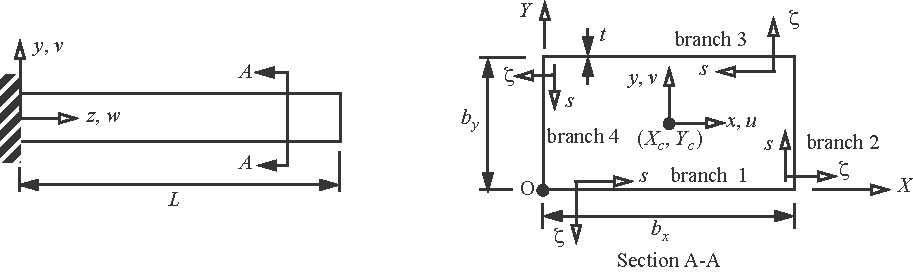
\includegraphics{Figure_8-7.pdf}}{\caption{Cantilever, thin-walled box beam.}\label{fig8.7}}

The lower horizontal flange, or branch 1, is a unidirectional
laminate with a ply angle $\varphi=-15^{\circ}$, and the upper
horizontal flange, or branch 3, is also a unidirectional laminate
with a ply angle of $\varphi=15^{\circ}$. The vertical webs, or
branches 2 and 4, are angle-ply laminates with a layup of
$\left(15^{\circ},-15^{\circ}\right)$. Imagine cutting the box
beam parallel to the $z$-axis through point~O. Then unfold the
laminated walls and lay them flat such that the outside surface is
facing up. The fiber directions with respect to $s$-$z$-$\zeta$
coordinates in each branch are shown in figure~\ref{fig8.8}.

\processfigure{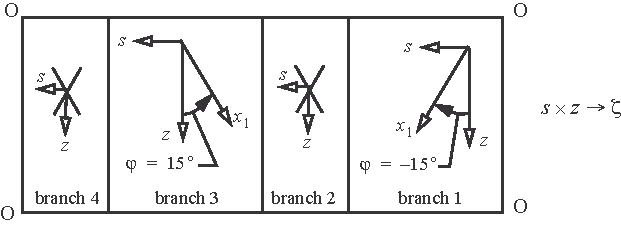
\includegraphics{Figure_8-8.pdf}}{\caption{Outside surface of\break the unfolded box.}\label{fig8.8}}

\begin{enumerate}[b)]%\leftskip=13pt
\item[{\hskip13pt}a)] Determine the torsional rotation $\phi_{z}(z)$ under
transverse bending $V_{y}=Q$.

\item[{\hskip13pt}b)] Determine the slope $d v/ d z$ of the reference axis due
to a torque $M_z$.
\end{enumerate}


\subsubsection{Solution.} Stiffness coefficients of the four
branches comprising the contour are listed in table~\ref{tab8.4}.



Note that $B_{3}=B_{1}$, $B_{4}=B_{2}$, $b_{3}=-b_{1}$,
$a_{3}=a_{1}$, and $a_{4}=a_{2}$. The origin of the contour
coordinate where $s=0$ is at point O of section A-A of
figure~\ref{fig8.7}. The Cartesian coordinate functions $(X(s),
Y(s))$ with origin also at point O are listed in
table~\ref{tab8.5}.

The axial stiffness is
\begin{align}\label{ex8.4a}
S=\oint B d s=2\left(B_{1} b_{x}+B_{2} b_{y}\right)=4.58819\,\mathrm{MN}.\tag{a}
\end{align}
The first moments with respect to the \textit{X-Y} coordinates are
\begin{align}\label{ex8.4b}
S_{X}=\oint B Y d s=b_{y}\left(B_{1} b_{x}+B_{2} b_{y}\right)
\quad S_{Y}=\oint B X d s=b_{x}\left(B_{1} b_{x}+B_{2}
b_{y}\right).\tag{b}
\end{align}
Consequently, the modulus-weighted centroid is located at

\vspace*{8pt}
\clearpage

\begin{table}%Table 8.4
\processtable{Stiffness coefficients for each branch of the box
beam\label{tab8.4}}
{\tabcolsep=8pt\begin{tabular}{@{}llll@{}}\toprule%
\colhead{Stiffness coefficient} & \multicolumn{1}{l}{\colhead{\textbf{Branch 1}}} &
\multicolumn{1}{l}{\colhead{\textbf{Branch 3}}} & \multicolumn{1}{l}{\colhead{\textbf{Branches 2 \& 4}}}\\
\midrule%
 $A_{11}$,  MN/m  & \phantom{$-$}8.59    & \phantom{0}8.59   & \phantom{0}8.59 \\
 $A_{12}$,  MN/m  & \phantom{$-$}8.93    & \phantom{0}8.93   & \phantom{0}8.93 \\
 $A_{22}$,  MN/m  & \phantom{$-$}9.67    & \phantom{0}9.67   & \phantom{0}9.67 \\
 $A_{66}$,  MN/m  & \phantom{\,}10.3    & 10.3   & 10.3 \\
 $A_{16}$,  MN/m  & $-$2.73 & \phantom{0}2.73   & \phantom{0}0    \\
 $A_{26}$,  MN/m  & $-$2.27 & \phantom{0}2.27   & \phantom{0}0    \\
 $B_{z}$,   MN/m  & \hspace*{-4.5pt}$-$19.9 & 19.8   & \phantom{0}0    \\
 $B_{s}$,   MN/m  & \phantom{$-$}9.46    & \phantom{0}9.455  & 10.3 \\
 $B$,       MN/m  & \hspace*{1pt}45.7    & 45.7   & 87.4 \\
 $b$, ($-$)       & $-$2.1  & \phantom{0}2.1    & \phantom{0}0    \\
 $a$, ($-$)         & \phantom{$-$}9.242   & \phantom{0}9.242  & \phantom{0}8.465\\
\botrule
\end{tabular}}{}\vspace*{-12pt}
\end{table}

\begin{table}%Table 8.5
\processtable{Parametric equations of the contour for the box
beam\label{tab8.5}} {\begin{tabular}{@{}llll@{}}\toprule%
\colhead{Branch no.} & \colhead{Range of $s$, in.} & \colhead{$X(s)$} & \colhead{$Y(s)$}\\
\midrule
 1 & $0 \leq s \leq b_{x}$ & $s$ & $0$\\
 2 & $b_{x} \leq s \leq b_{x}+b_{y}$ & $b_{x}$ & $s-b_{x}$\\
 3 & $b_{x}+b_{y} \leq s \leq 2 b_{x}+b_{y}$ & $2b_{x}+b_{y}-s$ & $b_{y}$\\
 4 & $2 b_{x}+b_{y} \leq s \leq 2(b_{x}+b_{y})$ & $0$ & $2(b_{x}+b_{y})-s$\\
\botrule
\end{tabular}}{}
\vspace*{-3\baselineskip}
\end{table}


\begin{align}\label{ex8.4c}
X_{c}=S_{Y}/ S=b_{x}/ 2 \quad Y_{c}=S_{X}/ S=b_{y}/ 2.\tag{c}
\end{align}
In this example the modulus-weighted centroid coincides with
the geometric centroid of the cross section. The Cartesian
coordinates of the contour with respect to the modulus-weighted
centroid are determined from $x(s)=X(s)-X_{c}$ and
$y(s)=Y(s)-Y_{c}$. The modulus-weighted second moments computed
from eq.~(\ref{eq8.57}) are
\begin{align}\label{ex8.4d}
D_{x x}=\frac{b_{y}^{2}}{6}(3 B_{1} b_{x}+B_{2}
b_{y})=138.884\,\mathrm{Nm}^{2} \quad D_{y
y}=\frac{b_{x}^{2}}{6}(B_{1} b_{x}+3 B_{2}
b_{y})=455.927\,\mathrm{Nm}^{2} \quad D_{x y}=0.\tag{d}
\end{align}
The
values of the parameters listed in eq.~(\ref{eq8.59}) are
$n_{x}=n_{y}=0$ and $k=1$. Hence, from eq.~(\ref{eq8.62}) we find
$\bar{x}(s)=x(s)$ and $\bar{y}(s)=y(s)$. Also, from
eq.~(\ref{eq8.69}) $\bar{S}_{x}(s)=S_{x}(s)$ and
$\bar{S}_{y}(s)=S_{y}(s)$. The modulus-weighted distribution
functions $S_{x}(s)$ and $S_{y}(s)$ with respect to a segment of
the cross-sectional area are defined in eq.~(\ref{eq8.70}), and
the results for these functions are listed in table~\ref{tab8.6}.\enlargethispage{2\baselineskip}

%Table 8.6
\begin{table}[!h]\vspace*{-6pt}
\processtable{Modulus-weighted distribution functions for the first area
moments\label{tab8.6}}
{\begin{tabular}{@{}lll@{}}\toprule
\colhead{\textbf{Branch}} & \colhead{$\bar{S}_{\textit{x}}(s)=S_{\textit{x}}(s)$} & \colhead{$\bar{S}_{\textit{y}}(s)=S_{\textit{y}}(s)$}\\
\midrule
 1 & $(-B_{1} b_{y} s)/ 2$ & $B_{1} s\left[(-b_{x}+s)/ 2\right]$\\[3pt]
 2 & $\left[-B_{1} b_{x} b_{y}+B_{2}(b_{x}-s)(b_{x}+b_{y}-s)\right]/2$ & $\left[B_{2} b_{x}(-b_{x}+s)\right]/ 2$\\[3pt]
 3 & $\left[-B_{1} b_{y}(2 b_{x}+b_{y}-s)\right]/ 2$ & $\left[B_{2} b_{x} b_{y}-B_{1}(2 b_{x}^{2}+3
b_{x}(b_{y}-s)+(b_{y}-s)^{2})\right]/
2$\\[3pt]
 4 & $-B_{2}(\left[4 b_{x}^{2}+6 b_{x} b_{y}+2 b_{y}^{2}-4
b_{x} s-3 b_{y}^{s}+s^{2}\right]/ 2)$ & $\left[B_{2}
b_{x}(2 b_{x}+2 b_{y}-s)\right]/ 2$\\
\botrule
\end{tabular}}{}
\vspace*{2pt}
\end{table}

\pagebreak

\noindent The procedure to determine $S_{x}(s)$ and $S_{y}(s)$ is the same
procedure used to determine the first area moments $Q_{x}(s)$ and
$Q_{y}(s)$ for a cross section with a wall made of an isotropic
material. See example~\ref{ex3.4} on page \pageref{ex3.4}. For the composite wall
$S_{x}(s)$ is analogous to $Q_{x}(s)$ of the isotropic wall, and
$S_{y}(s)$ is analogous to $Q_{y}(s)$. Note that
$\bar{S}_{x}(0)=0$ in branch 1, and that
$\bar{S}_{x}\!\left[2\left(b_{x}+b_{y}\right)\right]=0$ in branch 4,
which are necessary conditions for the first moment about the
centroidal $x$-axis. Similarly, $\bar{S}_{y}(0)=0$ in branch 1,
and $\bar{S}_{y}\!\left[2\left(b_{x}+b_{y}\right)\right]=0$ in
branch 4, which are necessary conditions for the first moment
about the centroidal $y$-axis.

The coordinates normal to the contour for each branch with respect
to the centroid given by eq.~(\ref{eq3.10}) on page \pageref{eq3.10}, and the
area enclosed by the contour, are as follows:
\begin{align}\label{ex8.4e}
r_{n c 1}=r_{n c 3}=b_{y}/ 2=6.8\,\mathrm{mm},\mbox{ }r_{n c
2}=r_{n c 4}=b_{x}/ 2=12.1\,\mathrm{mm}\mbox{, and }A_{c}=b_{x}
b_{y}=329.12\,\mathrm{mm}^{2}.\tag{e}
\end{align}
The numerical evaluation of
the shear flow distribution functions in eq.~(\ref{eq8.75}) can
now be computed with the results shown in table~\ref{tab8.7}.

%Table 8.7
\begin{table}[!h]
\vspace*{6pt}
\processtable{Shear flow distribution functions for the box beam\label{tab8.7}}
{\begin{tabular}{@{}lll@{}}\toprule
\colhead{Branch} & \colhead{$F_{x c}, m^{\boldsymbol -\textbf{1}} \text { (s in meters) }$} & \colhead{$F_{y
c}, m^{\boldsymbol -\textbf{1}} \text { (s in meters) }$}\\
\midrule
 1 & $-15.771-1{,}212.5 s+50{,}102.5 s^{2}$ & $-27.066-2{,}236.88 s$\\
 2 & $-71.896+2{,}319.2 s$ & $-260.728-19{,}505.9 s+314{,}612 s^{2}$\\
 3 & $-101.65+5{,}000.2 s-50{,}102.5 s^{2}$ & $-111.62+2{,}236.88 s$\\
 4 & $-159.564-2{,}319.24 s$ & $-1{,}447.58+43{,}290.5 s-314{,}612 s^{2}$\\
\botrule
\end{tabular}}{}\vspace*{-10pt}
\end{table}

For anisotropic wall properties, the normal stress resultant
(\ref{eq8.77}) is related to shear and torsion in addition to the
axial normal force and bending moments. The coefficient functions
of the shear terms ($\Phi_{x}(s)$ and $\Phi_{y}(s)$) and torsion
term ($\Phi(s)$) are given by eqs. (\ref{eq8.78}) to
(\ref{eq8.80}), and the numerical results for these functions are
listed below.

%Table 8.8
\begin{table}[!h]
\vspace*{6pt}
\processtable{Coefficient functions for shear and torsion
for the box beam (refer to eqs. (\ref{eq8.78}) to
(\ref{eq8.80})).\label{tab8.8}}
{\begin{tabular}{@{}llll@{}}\toprule
\colhead{\textbf{Branch}} & \colhead{$\Phi_{x}, m^{\boldsymbol -\textbf{1}}(\textrm{s} \text { in meters
})$} & \colhead{$\Phi_{y}, m^{\boldsymbol -\textbf{1}}(\mathrm{s} \text { in meters })$} & \colhead{$\Phi(s)$, \textbf{dimensionless and $s$ in meters}}\\
\midrule
 1 & $-12.209-2{,}546.37 s+105{,}222 s^{2}$ & $56.8427-4{,}697.75 s$ & $-0.554009$\\
 2 & $40.0001$ & 0 & $13.482-434.916 s$\\
 3 & $234.389-10{,}501.1 s+105{,}222 s^{2}$ & $234.418-4{,}697.75\,\mathrm{s}$ & $0.554009$\\
 4 & $40.0001$ & 0 & $-29.9222+434.916 s$\\
\botrule
\end{tabular}}{}\vspace*{-13pt}
\end{table}

The numerical result for the compliance matrix (\ref{eq8.104}) is
\begin{align*}
\left[\begin{array}{@{}c@{}}d \phi_{x}/ d z\\
d \phi_{y}/ d z\\
d w/ d z\\
\psi_{x}\\
\psi_{y}\\
d \phi_{z}/ d
z\end{array}\right]=10^{-3}\left[\begin{array}{@{}cccccc@{}}7.200
& 0 & 0 & 0 & 0 & -7.561\\
0 & 2.193 & 0 & 0 & 0 & 0\\
0 & 0 &
2.180 \times 10^{-4} & 4.577 \times 10^{-4} & 0 & 0\\
0 & 0 &
4.577 \times 10^{-4} & 3.389 \times 10^{-3} & 0 & 0\\
0 & 0 & 0 &
0 & 4.861 \times 10^{-3} & 0\\
-7.561 & 0 & 0 & 0 & 0 &
25.83\end{array}\right]\left[\begin{array}{@{}c@{}}M_{x}\\
M_{y}\\
N\\
V_{x}\\
V_{y}\\
M_{z}\end{array}\right].
\end{align*}
\vspace*{2pt}
\clearpage

The non-zero compliance coefficient $c_{16}$ couples the torsional
and bending responses of the beam. This coupling is illustrated in
the following numerical examples.
\begin{enumerate}[a.]\leftskip=3pt
\item[a.] Take the beam subject to transverse shear with $V_{y}=Q$, $0
\leq z \leq L$, and no other actions. The bending moment is
$M_{x}=-Q(L-z)$. The twist per unit length under transverse
bending is $d \phi_{z}/ d z=c_{61} M_{x}$. The torsional rotation
is given by
\begin{align*}
\phi_{z}=c_{61}\left[-Q\left(L
z-\frac{z^{2}}{2}\right)\right]=-c_{61} L^{2}
Q\left[\frac{z}{L}-\frac{1}{2}\left(\frac{z}{L}\right)^{2}\right]=0.00439
Q\left[\frac{z}{L}-\frac{1}{2}\left(\frac{z}{L}\right)^{2}\right].
\end{align*}
The distributions of the torsional rotation for $Q = 4.448$
N (1 lb.) from the present analysis, and from the experiment
conducted by Smith and Chopra (1991), are shown in figure~\ref{fig8.9}.

\processfigure{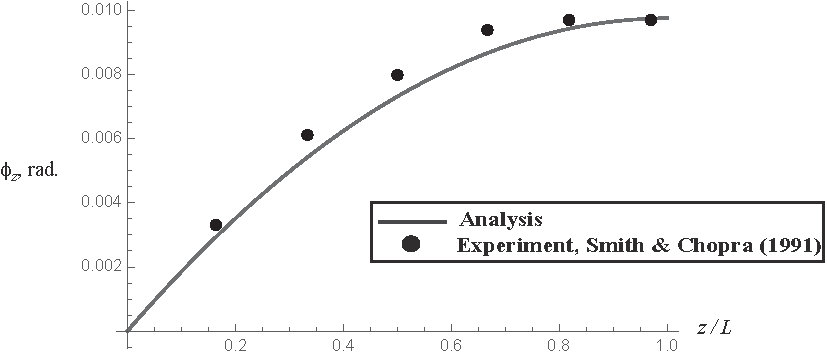
\includegraphics{Figure_8-9.pdf}}{\caption{Spanwise distribution of the torsional rotation for $V_y = Q = \textbf{4.448}$ N (1 lb.).}\label{fig8.9}}

\item[b.] Take the beam subject to a torque \textit{M}z and no other
actions. From the compliance matrix we find $\psi_{y}=c_{55} \cdot
0=0$. From eq.~(\ref{eq8.85}) the slope of the reference axis $d v
/ d z=-\phi_{x}$, and from the compliance matrix $d \phi_{x}/ d
z=c_{16} M_{z}$, and $\phi_{x}=c_{16} M_{z} z$. Since
$c_{16}=c_{61}$, the expression for the slope is
\begin{align*}
\frac{d v}{d
z}=-c_{61} M_{z} z=-(-7.561 \times 10^{-3}) L M_{z}(z/
L)=0.005761\left(\frac{1}{\mathrm{Nm}}\right) M_{z}(z/ L).
\end{align*}
The distributions of the slope of the reference axis from the
present analysis, and from the experiment conducted by Chandra et
al. (1990), for the torque $M_{z}=0.113\,\mathrm{Nm}$ (1.0 lb.-in.)
are shown in figure~\ref{fig8.10}.\quad\qed
\end{enumerate}
\end{example*}

\processfigure{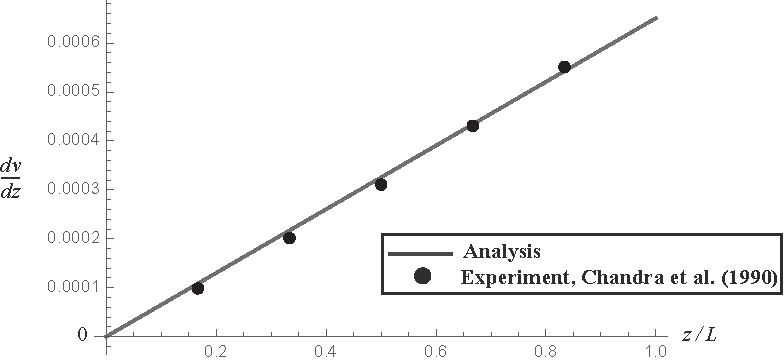
\includegraphics{Figure_8-10.pdf}}{\caption{Slope of the reference axis for an applied torque of 0.113 Nm (1.0 lb.-in.).}\label{fig8.10}}

\section{Open cross-sectional contour}\label{sec8.3}

For an open cross-sectional contour the shear flow is obtained
from eq.~(\ref{eq8.67}) on page \pageref{eq8.67}. The shear flow at the contour
origin $q_{0}=0$ if the origin is located at intersection with a
longitudinal free edge. (Refer to the discussion in article \ref{sec3.8.1}
on page \pageref{sec3.8.1}.) The equation for the shear flow for the FRP composite
bar is
\begin{align}\label{eq8.113}
q(s)=-\bar{S}_{x}(s) \frac{k}{D_{x x}} V_{y}-\bar{S}_{y}(s)
\frac{k}{D_{y y}} V_{x}.
\end{align}
The notes concerning the shear center in article \ref{sec3.8.3} on page \pageref{sec3.8.3}
apply as well to a bar made of an FRP composite. In particular
from these notes, the resultant of the shear flow distribution
over the contour is a force with components $V_x$ and
$V_y$ acting through the shear center such that there is no
torque acting at the shear center. If the cross section is subject
to a torque, this torque cannot be balanced by the shear flow,
which, according to eq.~(\ref{eq8.113}), is uniquely determined by
the shear forces $V_x$ and $V_y$. Part (b) of example
\ref{ex8.5} on page \pageref{ex8.5} shows how to find the shear center for an open
section starting with eq.~(\ref{eq8.113}). After locating the
shear center for the open cross-sectional contour, a material law
for the torque acting at the shear center remains to be
determined. This material law for torsion is developed in the next
section.

\section{Uniform torsion of an FRP bar with a rectangular cross section}\label{sec8.4}

We consider the uniform torsion of a prismatic bar with a
rectangular cross section composed of a linear elastic,
anisotropic material. Cartesian coordinates of the bar are denoted
by $s-z-\zeta$, where the coordinate $z$ is parallel to
the longitudinal axis of the bar. The origin of the coordinates
$s$ and $\zeta$ is at the center of the cross section; $-b/ 2 \leq s
\leq b/ 2$ where the width of the cross section is denoted by
$b$, and $-t/ 2 \leq \zeta \leq t/ 2$ where the thickness by
$t$. See figure~\ref{fig8.11}.

\vspace*{-10pt}

\processfigure{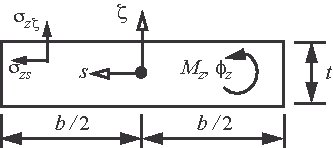
\includegraphics{Figure_8-11.pdf}}{\caption{Bar with a rectangular cross section subject to uniform torsion.}\label{fig8.11}}

\vspace*{-6pt}

The only applied load is a torque $M_{z}$ about the $z$-axis, and
the rotation about the $z$-axis corresponding to the torque is
denoted by $\phi_{z}$. The torque and rotation are positive
counterclockwise as shown in figure~\ref{fig8.11}. The shear stress
components acting on the cross section are denoted by $\sigma_{z
s}$ and $\sigma_{z \zeta}$, and the torque is related to the shear
stresses by the following integral over the cross section:
\begin{align}\label{eq8.114}
M_{z}=\int_{-b/ 2}^{b/ 2}\int_{-t/2}^{t/2}\left(\zeta
\sigma_{z s}-s \sigma_{z \zeta}\right) d \zeta d s.
\end{align}
\vspace*{2pt}
\clearpage

\noindent The lateral surfaces of the bar are not subject any loads or
tractions. Hence, the stress components must satisfy the following
conditions at the boundaries of the cross section:
\begin{gather}
\sigma_{\zeta s}=\sigma_{\zeta z}=\sigma_{\zeta \zeta}=0\mbox{, for }-b
/ 2 \leq s \leq b/ 2\mbox{ at }\zeta=\pm t/ 2. \label{eq8.115}\\
\sigma_{s s}=\sigma_{s z}=\sigma_{s \zeta}=0\mbox{, at }s=\pm b/ 2\mbox{ for }-t/ 2 \leq \zeta \leq t/ 2. \label{eq8.116}
\end{gather}
\textbf{Under uniform torsion all stress components and their
corresponding strains are independent of the axial coordinate $\textbf{\textit{z}}$.} The exact elasticity formulation for the anisotropic bar is
given in the monograph by Lekhnitskii (1981). We seek an
approximate solution based on the following assumptions:
\begin{itemize}
\item Stress components $\sigma_{s s}$, $\sigma_{s \zeta}$, and
$\sigma_{\zeta \zeta}$ are equal to zero in the domain of the
cross section.

\item The cross section is rigid in its own
plane.
\end{itemize}



The procedure to develop the material law is as
follows: (a) determine the displacements of the bar using the
strain-displacement relations and the anisotropic form of Hooke's
law, (b) satisfy the differential equation of equilibrium using a
separable form of the stress function, (c) use static equivalence
to determine the resultants of the axial normal stress, and (d)
impose the principle of complementary virtual work to find the
unknown part of the stress function. The final result for the
material law in torsion is given by eqs. (\ref{eq8.193}) and
(\ref{eq8.194}) on page \pageref{eq8.194}.


\subsection{Displacements}\label{sec8.4.1}

The non-zero stress components are the axial normal stress
$\sigma_{z z}$, and the shear stresses $\sigma_{z s}$ and
$\sigma_{z \zeta}$. To effect the rigidity assumption consider
Hooke's law (\ref{eq8.16}) for the strain components
$\varepsilon_{s s}$, $\varepsilon_{\zeta \zeta}$, and
$\gamma_{\zeta s}$. Write these material laws as
\begin{gather}\label{eq8.117}
\varepsilon_{s s} =\frac{\partial u_{s}}{\partial s}=\frac{1}{E_{s s}}\left[\sigma_{s s}+\left(\frac{C_{12}^{\prime}}{C_{11}^{\prime}}\right) \sigma_{z z}+\left(\frac{C_{13}^{\prime}}{C_{11}^{\prime}}\right) \sigma_{\zeta \zeta}+\left(\frac{C_{16}^{\prime}}{C_{11}^{\prime \prime}}\right) \sigma_{z s}\right] \nonumber\\
\varepsilon_{\zeta \zeta} =\frac{\partial u_{c}}{\partial \zeta}=\frac{1}{E_{\zeta \zeta}}\left[\left(\frac{C_{31}^{\prime}}{C_{33}^{\prime}}\right) \sigma_{s s}+\left(\frac{C_{32}^{\prime}}{C_{33}^{\prime}}\right) \sigma_{z z}+\sigma_{\zeta \zeta}+\left(\frac{C_{36}^{\prime}}{C_{33}^{\prime}}\right) \sigma_{z s}\right]\!,\\
\gamma_{\zeta s} =\frac{\partial u_{\zeta}}{\partial s}+\frac{\partial u_{s}}{\partial \zeta}=\frac{1}{G_{\zeta s}}\left[\left(\frac{C_{54}^{\prime}}{C_{55}^{\prime}}\right) \sigma_{z \zeta}+\sigma_{\zeta s}\right]\nonumber
\end{gather}
where $E_{ss}$ is the modulus of elasticity for
tension/compression along the $s$-axis, $E_{\zeta \zeta}$ is the
modulus along the $\zeta$-axis, and $G_{\zeta s}$ is the shear modulus
in the plane of the cross section. These moduli are related to the
compliance coefficients by $E_{s
s}=\left(C_{11}^{\prime}\right)^{-1}$, $E_{\zeta
\zeta}=\left(C_{33}^{\prime}\right)^{-1}$, and
$G_{\zeta_{5}}=\left(C_{55}^{\prime}\right)^{-1}$. Invoke the
rigidity of the cross section by letting $E_{ss} \rightarrow
\infty$, $E_{\zeta \zeta} \rightarrow \infty$, and $G_{\zeta_{s}}
\rightarrow \infty$. The assumption of a rigid cross-sectional
plane leads to the vanishing of the following strain-displacement
relations:
\begin{align}\label{eq8.118}
\varepsilon_{ss}=\frac{\partial u_{s}}{\partial s}=0 \quad
\varepsilon_{\zeta \zeta}=\frac{\partial u_{\zeta}}{\partial \zeta}=0
\quad \gamma_{\zeta s}=\frac{\partial u_{\zeta}}{\partial
s}+\frac{\partial u_{s}}{\partial \zeta}=0.
\end{align}
The normal strains in eq.~(\ref{eq8.118}) mean displacement
functions $u_{s}=u_{s}(z, \zeta)$ and $u_{\zeta}=u_{\zeta}(z, s)$.
Hooke's law (\ref{eq8.16}) for the remaining strains reduces to\vspace{-6pt}
\begin{gather}
\varepsilon_{z z}=\frac{\partial u_{z}}{\partial
z}=C_{22}^{\prime} \sigma_{z z}+C_{26}^{\prime} \sigma_{s z},\label{eq8.119}\\
\gamma_{z \zeta}=\frac{\partial u_{\tau}}{\partial
z}+\frac{\partial u_{z}}{\partial \zeta}=C_{44}^{\prime} \sigma_{z
\zeta}\mbox{, and }\label{eq8.120}\\
\gamma_{s z}=\frac{\partial u_{z}}{\partial s}+\frac{\partial
u_{s}}{\partial z}=C_{62}^{\prime} \sigma_{z z}+C_{66}^{\prime}
\sigma_{s z}.\label{eq8.121}
\end{gather}
Let the axial normal strain $\varepsilon_{z z}=D(s, \zeta)$, where
the function $D(s, \zeta)$ is to be determined from the
independence of the strains on axial coordinate \textit{z. }Begin
by integrating the strain-displacement equation for the axial
normal strain with respect to $z$ to determine the axial
displacement as
\begin{align}\label{eq8.122}
u_{z}=z D(s, \zeta)+w(s, \zeta).
\end{align}
Solve eq.~(\ref{eq8.119}), for the axial normal stress to get
\begin{align}\label{eq8.123}
\sigma_{z z}=\left(D-C_{26}^{\prime} \sigma_{z s}\right)
/\left(C_{22}^{\prime}\right).
\end{align}
Substitute the axial displacement (\ref{eq8.122}) into
eq.~(\ref{eq8.120}) to find
\begin{align}\label{eq8.124}
\frac{\partial u_{\zeta}}{\partial z}=-z \frac{\partial
D}{\partial \zeta}+\left(-\frac{\partial w}{\partial
\zeta}+C^{\prime}_{44} \sigma_{z \zeta}\right).
\end{align}
Integrate eq.~(\ref{eq8.124}) with respect to $z$ to get
\begin{align}\label{eq8.125}
u_{\zeta}=\frac{-z^{2}}{2} \frac{\partial D}{\partial
\zeta}+z\left(-\frac{\partial w}{\partial \zeta}+C^{\prime}_{44} \sigma_{z \zeta}\right)+v(s).
\end{align}
Substitute eq.~(\ref{eq8.125}) for the displacement $u_{\zeta}$
for the expression for the strain $\varepsilon_{\zeta \zeta}$ in
eq.~(\ref{eq8.118}) to get
\begin{align}\label{eq8.126}
\varepsilon_{\zeta \zeta}=\frac{\partial u_{\zeta}}{\partial
\zeta}=0=\frac{-z^{2}}{2} \frac{\partial^{2} D}{\partial
\zeta^{2}}+z \frac{\partial}{\partial \zeta}\left(-\frac{\partial
w}{\partial \zeta}+C^{\prime}_{44} \sigma_{z \zeta}\right),
\mbox{for all values of $z$.}
\end{align}
Substitute
eq.~(\ref{eq8.123}) for the axial normal stress into
eq.~(\ref{eq8.121}) to get
\begin{align}\label{eq8.127}
\gamma_{s z}=\frac{\partial u_{z}}{\partial s}+\frac{\partial
u_{s}}{\partial z}=\left(C_{62}^{\prime} D\right)/
C_{22}^{\prime}+\beta_{66} \sigma_{s z},
\end{align}
where $\beta_{66}=\left(C_{66}^{\prime}-C_{26}^{\prime 2}/
C_{22}^{\prime}\right)$. Substitute eq.~(\ref{eq8.122}) for
$u_{z}$ into eq.~(\ref{eq8.127}) to get
\begin{align}\label{eq8.128}
\frac{\partial u_{s}}{\partial z}=-z \frac{\partial D}{\partial
s}+\left(-\frac{\partial w}{\partial s}+\left(C_{62}^{\prime}
D\right)/ C_{22}^{\prime}+\beta_{66} \sigma_{s z}\right).
\end{align}
Integrate eq.~(\ref{eq8.128}) the with respect to $z$ to find the
displacement $u_{s}$ as
\begin{align}\label{eq8.129}
u_{s}=\frac{-z^{2}}{2} \frac{\partial D}{\partial
s}+z\left(-\frac{\partial w}{\partial s}+\beta_{66} \sigma_{s
z}+\left(C_{62}^{\prime} D\right)/
C_{22}^{\prime}\right)+u(\zeta).
\end{align}
Substitute eq.~(\ref{eq8.129}) for displacement $u_{s}$ in the
expression for the strain $\varepsilon_{s s}$ in
eq.~(\ref{eq8.118}) to get
\begin{align}\label{eq8.130}
\varepsilon_{s s}=\frac{\partial u_{s}}{\partial
s}=0=\frac{-z^{2}}{2}\left(\frac{\partial^{2} D}{\partial
s^{2}}\right)+z \frac{\partial}{\partial s}\left(-\frac{\partial
w}{\partial s}+\beta_{66} \sigma_{s z}+\left(C_{62}^{\prime}
D\right)/ C_{22}^{\prime}\right)\mbox{, for all values of $z$.}
\end{align}
Substitute displacement $u_{\zeta}$ from
eq.~(\ref{eq8.125}), and substitute displacement $u_{s}$ from
eq.~(\ref{eq8.129}), into the expression for the shear strain
$\gamma_{\zeta s}$ in eq.~(\ref{eq8.118}) to get
\begin{align}\label{eq8.131}
\gamma_{\zeta s}=0=-z^{2} \frac{\partial^{2} D}{\partial s
\partial \zeta}+z\left[\frac{\partial}{\partial
s}\left(-\frac{\partial w}{\partial \zeta}+C_{44}^{\prime}
\sigma_{z \zeta}\right)+\frac{\partial}{\partial
\zeta}\left(-\frac{\partial w}{\partial s}+\beta_{66} \sigma_{s
z}+\left(C_{62}^{\prime} D\right)/ C^{\prime}_{22}\right)\right]+\frac{d v}{d s}+\frac{d u}{d \zeta}.
\end{align}
Equations (\ref{eq8.126}), (\ref{eq8.130}), and (\ref{eq8.131})
are to be satisfied for all values of $z$, from which we conclude
the following results:
\begin{gather}
\frac{\partial^{2} D}{\partial \zeta^{2}}=0 \quad
\frac{\partial^{2} D}{\partial s^{2}}=0 \quad \frac{\partial^{2}
D}{\partial s \partial \zeta}=0\label{eq8.132}\\
\frac{\partial}{\partial \zeta}\left(-\frac{\partial w}{\partial
\zeta}+C_{44}^{\prime} \sigma_{z \zeta}\right)=0 \quad
\frac{\partial}{\partial s}\left(-\frac{\partial w}{\partial
s}+\beta_{66} \sigma_{s z}+\left(C_{62}^{\prime} D\right)/
C_{22}^{\prime}\right)=0\label{eq8.133}\\
\frac{\partial}{\partial s}\left(-\frac{\partial w}{\partial
\zeta}+C^{\prime}_{44} \sigma_{z
\zeta}\right)+\frac{\partial}{\partial \zeta}\left(-\frac{\partial
w}{\partial s}+\beta_{66} \sigma_{s z}+\left(C^{\prime}_{62}
D\right)/ C_{22}^{\prime}\right)=0 \quad \frac{d v}{d s}+\frac{d
u}{d \zeta}=0.\label{eq8.134}
\end{gather}
To satisfy the vanishing of partial derivatives of \textit{D} in
eq.~(\ref{eq8.132}), we find that function \textit{D} is linear in
the coordinates. That is,
\begin{align}\label{eq8.135}
D=\bar{A} s+\bar{B} \zeta+\bar{C},
\end{align}
where $\bar{A}$, $\bar{B}$, and $\bar{C}$ are
constants that will be determined later. Integrate the second
expression eq.~(\ref{eq8.133}) with respect to $s$, and then
integrate the first expression in eq.~(\ref{eq8.133}) with respect
to $\zeta$. The results of these integrations are
\begin{gather}
-\frac{\partial w}{\partial s}+\beta_{66} \sigma_{s
z}+\left(C_{62}^{\prime} D\right)/
C_{22}^{\prime}+F_{1}(\zeta)=0\mbox{, and}\label{eq8.136}\\
-\frac{\partial
w}{\partial \zeta}+C_{44}^{\prime} \sigma_{z \zeta}+F_{2}(s)=0.\label{eq8.137}
\end{gather}
Substitute eq.~(\ref{eq8.136}) and eq.~(\ref{eq8.137}) into the
first expression in eq.~(\ref{eq8.134}) to find
\begin{align}\label{eq8.138}
\frac{d F_{1}}{d \zeta}+\frac{d F_{2}}{d s}=0.
\end{align}
Equation (\ref{eq8.138}) is satisfied by $F_{1}(\zeta)=-\lambda\;
\zeta$ and $F_{2}(s)=\lambda s$, where $\lambda$ is called a separation
constant. Substitute the result for ${F}_1$ into
eq.~(\ref{eq8.136}) to find
\begin{align}\label{eq8.139}
\frac{\partial w}{\partial s}=\beta_{66} \sigma_{s
z}+\left(C_{62}^{\prime} D\right)/ C_{22}^{\prime}-\lambda\;\zeta.
\end{align}
Substitute the result for $F_2$ into eq.~(\ref{eq8.137}) to
find
\begin{align}\label{eq8.140}
\frac{\partial w}{\partial \zeta}=C_{44}^{\prime} \sigma_{z
\zeta}+\lambda s.
\end{align}
Substitute the derivative of displacement $w$ with respect to $\zeta$
from eq.~(\ref{eq8.140}) into the displacement $u_{\zeta}$ given
in eq.~(\ref{eq8.125}) to get
\begin{align}\label{eq8.141}
u_{\zeta}=\frac{-z^{2}}{2} \bar{B}-\lambda z s+v(s).
\end{align}
Substitute the derivative of displacement $w$ with respect to
\textit{s} from eq.~(\ref{eq8.139}) into the displacement $u_{s}$
given in eq.~(\ref{eq8.129}) to get
\begin{align}\label{eq8.142}
u_{s}=\frac{-z^{2}}{2} \bar{A}+\lambda z \zeta+u(\zeta).
\end{align}
From eq.~(\ref{eq8.134}) consider the relation $\frac{d v}{d
s}+\frac{d u}{d \zeta}=0$. The latter relation is satisfied by
$\frac{d v}{d s}=-\omega$ and $\frac{d u}{d \zeta}=\omega$, where
$\omega$ is a second separation constant. Thus, $v(s)=-\omega
s+v(0)$ and $u(\zeta)=\omega \zeta+u(0)$. Substitute the equations
for $v(s)$ and $u(\zeta)$ into eqs. eq.~(\ref{eq8.141})and
eq.~(\ref{eq8.142}) to get
\begin{align}\label{eq8.143}
u_{\zeta}=\frac{-z^{2}}{2} \bar{B}-\lambda z s-\omega s+v(0) \quad
u_{s}=\frac{-z^{2}}{2} \bar{A}+\lambda z \zeta+\omega \zeta+u(0).
\end{align}

\begin{wrapfigure}[11]{L}{122pt}
\vspace{-24pt}
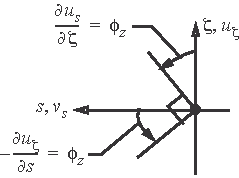
\includegraphics{Figure_8-12.pdf}
\caption{Rotation of the cross section about the\break $z$-axis.\label{fig8.12}}
\end{wrapfigure}

\noindent
From eq.~(\ref{eq8.118}) the in-plane shear strain $\gamma_{\zeta
s}=\frac{\partial u_{\zeta}}{\partial s}+\frac{\partial
u_{s}}{\partial \zeta}=0$. As shown in figure~\ref{fig8.12} the partial
derivative terms appearing in the shear strain can be related to
rotation $\phi_{z}$ of the cross section. Let $\frac{\partial
u_{s}}{\partial \zeta}=\phi_{z}$ and let $-\frac{\partial
u_{z}}{\partial s}=\phi_{z}$. The partial derivatives of the
displacements in eq.~(\ref{eq8.143}) are equated to the rotation
to get
\begin{align}\label{eq8.144}
\phi_{z}=\frac{\partial u_{s}}{\partial \zeta}=\lambda z+\omega\mbox{,
and }\phi_{z}=-\frac{\partial u_{\zeta}}{\partial s}=\lambda
z+\omega .
\end{align}
\noindent Thus, $\phi_{z}=\lambda z+\omega$, from which we identify the
separation constant $\lambda=\frac{d \phi_{z}}{d z}$. The
separation constant $\omega$ represents a rigid body rotation of
the bar about the $z$-axis. To prevent rigid body rotation and
displacement of the cross section set $\omega=0$, $v(0)=0$, and
$u(0)=0$. The final results for the displacements are
\begin{gather}
u_{z}=z(\bar{A} s+\bar{B} \zeta+\bar{C})+w(s, \zeta),\label{eq8.145}\\
u_{\zeta}=\frac{-z^{2}}{2} \bar{B}-z s \frac{d \phi_{z}}{d z}\mbox{, and }\label{eq8.146}\\
u_{s}=\frac{-z^{2}}{2} \bar{A}+z \zeta \frac{d \phi_{z}}{d z}.\label{eq8.147}
\end{gather}

\subsection{Equilibrium}\label{sec8.4.2}

The differential equation for axial equilibrium is
\begin{align}\label{eq8.148}
\frac{\partial \sigma_{s z}}{\partial s}+\frac{\partial
\sigma_{\zeta} z}{\partial \zeta}+\underbrace{\frac{\partial
\sigma_{z z}}{\partial z}}_{=0}=0.
\end{align}
The axial normal stress $\sigma_{z z}$ does not contribute to
eq.~(\ref{eq8.148}) since it is independent of coordinate $z$.
Equation (\ref{eq8.148}) is identically satisfied by the
introduction of the stress function $\psi(s, \zeta)$ where the
stress components are related to the stress function by
\begin{align}\label{eq8.149}
\sigma_{s z}=-\frac{\partial \psi}{\partial \zeta} \quad
\sigma_{\zeta z}=\frac{\partial \psi}{\partial s}.
\end{align}
For shear stress $\sigma_{\zeta z}$ to satisfy the boundary
conditions (\ref{eq8.115}) at $\zeta=\pm t/ 2$ the stress
function $\partial \psi/ \partial s=0$. For shear stress
$\sigma_{s z}$ to satisfy the boundary conditions (\ref{eq8.116})
at $s=\pm b/ 2$ the stress function $\partial \psi/ \partial
\zeta=0$. That is the stress function is a constant on the
boundaries, and for convenience we take $\psi=0$ on the boundaries
of the rectangular domain.

Substitute eq.~(\ref{eq8.149}) for the shear stresses in the
expression (\ref{eq8.114}) for the torque to get
\begin{align}\label{eq8.150}
M_{z}=\int_{-b/ 2}^{b/ 2}\left[\int_{-t/ 2}^{t/
2}\left(\zeta\left(-\frac{\partial \psi}{\partial
\zeta}\right)-s\left(\frac{\partial \psi}{\partial
s}\right)\right) d \zeta\right].
\end{align}
\vspace*{2pt}
\clearpage

\noindent Integrate eq.~(\ref{eq8.150}) by parts with respect to $s$ and $\zeta$ to get
\begin{align}\label{eq8.151}
M_{z}=\int_{-b/ 2}^{b/ 2}\left\{-\left.\zeta \psi\right|_{t/ 2}
^{t/ 2}+\int_{-t/ 2}^{t/ 2} \psi d \zeta\right\} d s+\int_{-t/
2}^{t/ 2}\left\{\left.[-s \psi]\right|_{-b/ 2} ^{b/ 2}+\int_{-b
/ 2}^{t/ 2} \psi d s\right\} d \zeta.
\end{align}
Since the stress function is equal to zero on the boundaries we
find that the torque is given by integral of the stress function
over the cross-sectional area:
\begin{align}\label{eq8.152}
M_{z}=2 \int_{-b/ 2}^{b/ 2} \int_{-t/ 2}^{t/ 2} \psi d \zeta d
s.
\end{align}
We make an additional assumption for the stress function that
\begin{align}\label{eq8.153}
\psi(s, \zeta)=\psi_{1}(s)\left[(t/ 2)^{2}-\zeta^{2}\right],
\end{align}
which satisfies the boundary condition that $\psi(s, \pm t/
2)=0$. Function $\psi_{1}(s)$ must satisfy the boundary condition
$\psi_{1}(\pm b/ 2)=0$. The shear stresses for this assumption
are given by
\begin{align}\label{eq8.154}
\sigma_{s z}=2 \psi_{1}(s) \zeta \quad \sigma_{\zeta z}=\frac{d
\psi_{1}}{d s}\left[(t/ 2)^{2}-\zeta 2\right].
\end{align}
Substitute the stress function (\ref{eq8.153}) into the torque
(\ref{eq8.152}) to get
\begin{align}\label{eq8.155}
M_{z}=\frac{t^{3}}{3} \int_{-b/ 2}^{b/ 2} \psi_{1}(s) d s.
\end{align}

\subsection{Static equivalence}\label{sec8.4.3}

In general, the resultants of the axial normal stress
$\sigma_{z z}$ acting over the cross section are a normal force
denoted by \textit{N}, a bending moment about the $s$-axis by
$M_{s}$, and a bending moment about the $\zeta$-axis by $M_{\zeta}$.
For a laminated wall these resultants are given by
\begin{align}\label{eq8.156}
\left(N, M_{\zeta}, M_{s}\right)=\int_{-b/ 2}^{b/
2}\left[\sum_{k=1}^{N p} \int^{\zeta_{k+1}}_{\zeta_{k}}(1, \zeta,
s) \sigma_{z z}^{(k)} d \zeta\right] d s,
\end{align}
where $N_{p}$ is the number of plies, and $k=1,2, \ldots,\; N_{p}$.
At the bottom of the \textit{k-th} ply $\zeta=\zeta_{k}$, and at
the top of the \textit{k-th} ply $\zeta=\zeta_{k+1}$,
$\zeta_{k+1}>\zeta_{k}$. From eqs. (\ref{eq8.123}) and
(\ref{eq8.149}) the axial normal stress in the \textit{k-th} ply
is
\begin{align}\label{eq8.157}
\sigma_{z
z}^{(k)}=\frac{D}{C_{22}^{\prime}(k)}-\left(\frac{C_{26}^{\prime}}{C_{22}^{\prime}}\right)^{(k)}
\sigma_{s z}=\frac{(\bar{A} s+\bar{B}
\zeta+\bar{C})}{C_{22}^{\prime}(k)}-\left(\frac{C_{26}^{\prime}}{C_{22}^{\prime}}\right)^{(k)}
2 \zeta \psi_{1}(s).
\end{align}
Substitute eq.~(\ref{eq8.157}) for the axial normal stress into
the equations for the axial force and bending moments given by
eq.~(\ref{eq8.156}). In the process of computing the resultants,
integrals that are explicit in coordinates $s$ and $\zeta$ are
performed. Integrals of the stress function also appear in this
process and from eq.~(\ref{eq8.155}), and we use the fact that
\begin{align*}
\int_{-b/ 2}^{b/ 2} \psi_{1}(s) d s=\frac{3 M_{z}}{t^{3}}.
\end{align*}
The results are
\begin{gather}
N=\left(b B_{22}\right) \bar{B}+\left(b A_{22}\right)
\bar{C}-\frac{6}{t^{3}} \theta_{26} M_{z},\label{eq8.158}\\
M_{s}=\left(b D_{22}\right) \bar{B}+\left(b B_{22}\right)
\bar{C}-\eta_{26} M_{z}\mbox{, and}\label{eq8.159}\\
M_{\zeta}=\left(\frac{b^{3}}{12} A_{22}\right) \bar{A}-2
\theta_{26} \int_{-b/ 2}^{b/ 2} s \psi_{1}(s) d s.\label{eq8.160}
\end{gather}
Stiffness coefficients in the previous equations are defined by
\begin{align}\label{eq8.161}
A_{22}=\sum_{k=1}^{Np}
\frac{1}{C_{22}^{\prime}(k)}\left(\zeta_{k+1}-\zeta_{k}\right)
\quad B_{22}=\sum_{k=1}^{Np} \frac{1}{2
C_{22}^{\prime}(k)}\big(\zeta_{k+1}^{2}-\zeta_{k}^{2}\big)
\quad D_{22}=\sum_{k=1}^{Np} \frac{1}{3 C^{\prime(k)}_{22}}\big(\zeta_{k}^{3}+1-\zeta_{k}^{3}\big).
\end{align}
Shear-extension coupling coefficients are defined by
\begin{align}\label{eq8.162}
\theta_{26}=\sum_{k=1}^{Np}\left(\frac{C_{26}^{\prime}}{C_{22}^{\prime}}\right)^{(k)}
\frac{1}{2}\big(\zeta_{k+1}^{2}-\zeta_{k}^{2'}\big) \quad
\eta_{26}=\left(\frac{6}{t^{3}}\right) \sum_{k=1}^{Np}\left(\frac{C_{26}^{\prime}}{C_{22}^{\prime}}\right)^{(k)}
\frac{1}{3}\big(\zeta_{k+1}^{3}-\zeta_{k}^{3}\big).
\end{align}
We limit consideration to a \textbf{symmetric laminate} in which
the stacking sequence of the plies is symmetric about the
midplane. Symmetry leads to coefficients
\begin{align}\label{eq8.163}
B_{22}=\theta_{26}=0.
\end{align}
To illustrate that symmetry results in the previous property
consider two identical plies labeled \textit{K} and \textit{L} in
figure~\ref{fig8.13}. The two plies have the same material properties,
same thickness denoted by $h$, and are symmetrically located with
respect to the midplane. Symmetry requires the coordinates
$\zeta_{L}+ \zeta_{K+1}=0$. The remaining coordinates are
$\zeta_{K}=\zeta_{K+1}-h$ and $\zeta_{L+1}=\zeta_{L}+h$. The sum
the of plies \textit{K} and \textit{L} that contribute to
coefficient $B_{22}$ are

\vspace*{-10pt}

\processfigure[!h]{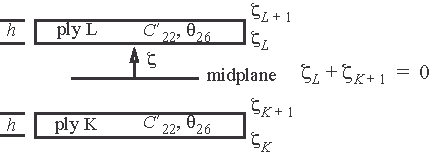
\includegraphics{Figure_8-13.pdf}}{\caption{Identical plies symmetric about the midplane.}\label{fig8.13}}

\vspace*{-2.5pc}

\begin{align}\label{eq8.164}
\frac{1}{2
C_{22}^{\prime}}\left[\zeta_{L+1}^{2}-\zeta_{L}^{2}+\zeta_{K+1}^{2}-\zeta_{K}^{2}\right]=\frac{1}{2
C_{22}^{\prime}}\left[\left(\zeta_{L}+h\right)^{2}-\zeta_{L}^{2}+\left(-\zeta_{L}\right)^{2}-\left(-\zeta_{L}-h\right)^{2}\right]=0.
\end{align}
\noindent Hence, for a symmetric laminate the normal force $N=0$ leads to
coefficient $\bar{C}=0$, bending moment $M_{\zeta}=0$ leads to
coefficient $\bar{A}=0$, and bending moment $M_{s}=0$ leads to
coefficient $B$ given by
\begin{align}\label{eq8.165}
\bar{B}=\frac{\eta_{26}}{b D_{22}} M_{z}.
\end{align}
The transverse shear resultants acting on the cross section are
denoted by $V_{s}$ and $V_{\zeta}$. They are given by
\begin{align}\label{eq8.166}
V_{s}=\int_{-b/ 2}^{b/2}\left[\int_{-t/ 2}^{t/ 2} \sigma_{z
s} d \zeta\right] d s\mbox{ and }V_{\zeta}=\int_{-t/ 2}^{t/
2}\left[\int_{-b/ 2}^{b/ 2} \sigma_{z \zeta} d s\right] d \zeta.
\end{align}
Substitute eq.~(\ref{eq8.154}) for the shear stresses in the
integrals of the previous equations to get
\begin{gather}
V_{s}=\int_{-b/ 2}^{b/ 2} 2 \psi_{1}\left[\int_{-t/ 2}^{t/ 2}
\zeta d \zeta\right] d s=\int_{-b/ 2}^{b/ 2} 2 \psi_{1}[0] d
s=0\mbox{, and }\label{eq8.167}\\*
\nonumber\\
V_{\zeta}=\int_{-t/ 2}^{t/ 2}\left\{\left[t/
2^{2}-\zeta^{2}\right]\left[\int_{-b/ 2}^{b/ 2} \frac{d
\psi_{1}}{d s} d s\right]\right\} d \zeta=\int_{-t/ 2}^{t/
2}\left\{\left[t/ 2^{2}-\zeta^{2}\right]\left[\psi_{1}(b/
2)-\psi_{1}(-b/ 2)\right]\right\} d \zeta=0.\label{eq8.168}
\end{gather}
Therefore, the resultants acting on the cross section of the bar
are $N=V_{s}=V_{\zeta}=M_{s}=M_{\zeta}=0$ and an applied torque
$M_{z} \neq 0$.

\subsection{Principle of complementary virtual work}\label{sec8.4.4}

Consider uniform torsion state of the bar as shown in
figure. \ref{fig8.11} where the displacements, strains, and forces satisfy
the compatibility conditions, Hooke's law, and the equilibrium
conditions. In this state, the actual displacements are $u_{z},
u_{\zeta}$, and $u_{s}$ given by eqs. (\ref{eq8.145}),
(\ref{eq8.146}), and (\ref{eq8.147}), respectively. The actual
non-zero strains are $\varepsilon_{z z}, \gamma_{z \zeta}, \text {
and } \gamma_{s z}$ and the corresponding stresses are $\sigma_{z
z}, \sigma_{z \zeta}, \text { and } \sigma_{s z}$, respectively.
The only cross-sectional resultant is the torque $M_{z}$ and its
corresponding rotation is $\phi_{z}$. Now consider infinitesimal
increments in the stresses denoted by $\delta \sigma_{z z}, \delta
\sigma_{z \zeta}, \text { and } \delta \sigma_{s z}$ that satisfy
equilibrium. For a bar of length \textit{L,} $0 \leq z \leq L$,
the increment in the internal complementary work is given by
\begin{align}\label{eq8.169}
\delta W_{\text {int }} &=
\int_{0}^{L}\left\{\int_{-b/ 2}^{b/ 2}
\int_{-t/2}^{t/ 2}
\left(\varepsilon_{z z} \delta \sigma_{z
z}+\gamma_{z \zeta} \delta \sigma_{z \zeta}+\gamma_{s z} \delta
\sigma_{s z}\right) d \zeta d s\right\} d z\nonumber\\
&=L
\int_{-b/ 2}^{b/ 2}\int_{-t/2}^{t/ 2} \left(\varepsilon_{z z} \delta
\sigma_{z z}+\gamma_{z \zeta} \delta \sigma_{z \zeta}+\gamma_{s z}
\delta \sigma_{s z}\right) d \zeta d s,
\end{align}
Note that the strains and stresses are independent of the axial
coordinate $z$. The increment in the external complementary work
is
\begin{align}\label{eq8.170}
\delta W_{\text {ext }} &=\left.
\int_{-b/ 2}^{b/ 2}\int_{-t/2}^{t/ 2}
\left(u_{z} \delta \sigma_{z z}+u_{\zeta}
\delta \sigma_{z \zeta}+u_{s} \delta \sigma_{z
s}\right)\right|_{z=L} d \zeta d s\nonumber\\
&-\left.\int_{-b/ 2}^{b/ 2}\int_{-t/2}^{t/ 2}\left(u_{z} \delta \sigma_{z z}+u_{\zeta} \delta \sigma_{z
\zeta}+u_{s} \delta \sigma_{z s}\right)\right|_{z=0} d \zeta d s.
\end{align}
From eqs. (\ref{eq8.145}) to (\ref{eq8.147}), and with
displacement coefficients $\bar{A}=\bar{C}=0$, the displacements
at the end cross sections are as follows:
\begin{gather}
\mbox{At }z=0, u_{z}=w(s, \zeta), u_{\zeta}=0\mbox{, and } u_{s}=0.\label{eq8.171}\\
\mbox{At }z=L, u_{z}=L \bar{B} \zeta+w(s, \zeta),
u_{\zeta}=-\frac{L^{2} \bar{B}}{2}-L s \frac{d \phi_{z}}{d z}\mbox{, and }u_{s}=L \zeta \frac{d \phi_{z}}{d z}.\label{eq8.172}
\end{gather}
Substitute the displacements at $z=0$ and $z=L$ into the increment
in the external work (\ref{eq8.170}) to get
\begin{align*}
\delta W_{\text {ext }}=&
\int_{-b/ 2}^{b/ 2}\int_{-t/2}^{t/ 2}
\left[(L \bar{B} \zeta+w(s, \zeta)) \delta \sigma_{z
z}+\left(-\frac{L^{2} \bar{B}}{2}-L s \frac{d \phi_{z}}{d
z}\right) \delta \sigma_{z \zeta}+\left(L \zeta \frac{d
\phi_{z}}{d z}\right) \delta \sigma_{z s}\right] d \delta d
s\nonumber\\
&-\int_{-b/ 2}^{b/ 2}\int_{-t/2}^{t/ 2}\left[w(s, \zeta) \delta
\sigma_{z z}\right] d \zeta d s,
\end{align*}
in which we used the fact that the increments in the stresses are
independent of the coordinate $z$. The integrals involving $w
\delta \sigma_{z z}$ add to zero. Hence,
\begin{align*}
\delta W_{\mathrm{ext}}=\int_{-b/ 2}^{b/ 2}\int_{-t/2}^{t/ 2}
\left[(L \bar{B} \zeta) \delta \sigma_{z
z}+\left(-\frac{L^{2} \bar{B}}{2}-L s \frac{d \phi_{z}}{d
z}\right) \delta \sigma_{z \zeta}+\left(L \zeta \frac{d
\phi_{z}}{d z}\right) \delta \sigma_{z s}\right] d \zeta d s.
\end{align*}
Rearrange the terms in the last equation, and note displacement
coefficient $\bar{B}$ is a constant, to get
\begin{align}\label{eq8.173}
\delta W_{\text {ext }}=L \bar{B} \int_{-b/ 2}^{b/ 2}\int_{-t/2}^{t/ 2} \zeta \delta \sigma_{zz} d \zeta d s-\frac{L^{2}
\bar{B}}{2} \int_{-b/ 2}^{b/ 2}\int_{-t/2}^{t/ 2} \delta\sigma_{z\zeta} d \zeta d s+L \frac{d \phi_{z}}{d z} \int_{-b/ 2}^{b/ 2}\int_{-t/2}^{t/ 2}\left(\zeta \delta \sigma_{z s}-s \delta
\sigma_{z \zeta}\right) d \zeta d s.
\end{align}
Integrals of the increments in the stresses are identified as
increments in the resultants $\delta M_{s}$, $\delta V_{\zeta}$,
and $\delta M_{z}$. Then, we find
\begin{align}\label{eq8.174}
\delta W_{\text {ext }}=L \bar{B} \delta M_{s}-\frac{L^{2}
\bar{B}}{2} \delta V_{\zeta}+L \frac{d \phi_{z}}{d z} \delta
M_{z}.
\end{align}
Since the bending moment $M_{s}$ is prescribed then $\delta
M_{s}=0$. Similarly, shear force $V_{\zeta}$ is prescribed, so
$\delta V_{\zeta}=0$. The final expression for the increment in
the external work is
\begin{align}\label{eq8.175}
\delta W_{\text {ext }}=L \frac{d \phi_{z}}{d z} \delta M_{z}.
\end{align}
Equate the increment in the external work (\ref{eq8.175}) to the
increment in internal work (\ref{eq8.169}), followed by division
by \textit{L}, to get the principle of complementary work as
\begin{align}\label{eq8.176}
\frac{d \phi_{z}}{d z} \delta M_{z}=\int_{-b/ 2}^{b/ 2}\int_{-t/2}^{t/ 2}
\left(\varepsilon_{z z} \delta \sigma_{z z}+\gamma_{z
\zeta} \delta \sigma_{z \zeta}+\gamma_{s z} \delta \sigma_{s
z}\right) d \zeta d s.
\end{align}

\vspace*{-1pc}

The strain-stress relations are given by Hooke's law in eqs.
(\ref{eq8.119}) to (\ref{eq8.121}). In Hooke's law for the strains
$\varepsilon_{z z}$ and $\gamma_{s z}$ we substitute
eq.~(\ref{eq8.123}) for the axial normal stress. After the process
of eliminating the axial normal stress, we get the strain
relations as
\begin{align}\label{eq8.177}
\varepsilon_{z z}=\bar{B} \zeta \quad \gamma_{z \zeta}=C^{\prime}_{44} \sigma_{z \zeta} \quad \gamma_{s
z}=\left(\frac{C^{\prime}_{26}}{C^{\prime}_{22}}\right) \bar{B}
\zeta+\beta_{66} \sigma_{s z},
\end{align}
where the compliance coefficient
$\beta_{66}=C_{66}^{\prime}-C_{26}^{\prime 2}/ C_{22}^{\prime}$.
Let $\bar{B} \rightarrow \bar{B}+\delta \bar{B}$ and $\sigma_{s z}
\rightarrow \sigma_{s z}+\delta \sigma_{s z}$ in
eq.~(\ref{eq8.123}) to find that the increment in the normal
stress is
\begin{align}\label{eq8.178}
\delta \sigma_{z z}=\frac{\zeta}{C_{22}^{\prime}} \delta
\bar{B}-\frac{C_{26}^{\prime}}{C_{22}^{\prime}} \delta \sigma_{s
z}.
\end{align}
Substitute eq.~(\ref{eq8.177}) for the strains in
eq.~(\ref{eq8.176}), followed by substitution of
eq.~(\ref{eq8.178}) for the increment in the normal stress. The
result of these substitutions is the following form for the
principle of complementary work:
\begin{align}\label{eq8.179}
\frac{d \phi_{z}}{d z} \delta M_{z}=\int_{-b/ 2}^{b/
2}\left\{\int_{t/ 2}^{t/
2}\left[\left(\frac{\zeta^{2}}{C^{\prime}} \bar{B}\right) \delta
\bar{B}+\left(C^{\prime}_{44} \sigma_{z \zeta}\right) \delta
\sigma_{z \zeta}+\left(\beta_{66} \sigma_{s z}\right) \delta
\sigma_{s z}\right] d \zeta\right\} d s.
\end{align}
Statically admissible increments $\delta \sigma_{z s}$ and $\delta
\sigma_{z \zeta}$ in eq.~(\ref{eq8.179}) are defined in terms of
the increment in the stress function $\delta \psi_{1}$ by
\begin{align}\label{eq8.180}
\delta \sigma_{s z}=2 \zeta \delta \psi_{1}(s) \quad \delta
\sigma_{z \zeta}=\delta\left(\frac{d \psi_{1}}{d
s}\right)\left[\left(\frac{t}{2}\right)^{2}-\zeta^{2}\right].
\end{align}
Substitute eq.~(\ref{eq8.180}) for the increments in the stresses
in eq.~(\ref{eq8.179}), followed by the substituting of
eq.~(\ref{eq8.154}) for the stresses $\sigma_{s z}$ and $\sigma_{z
\zeta}$ in eq.~(\ref{eq8.179}). The result of these substitutions
is
\begin{align}\label{eq8.181}
\frac{d \phi_{z}}{d z} \delta M_{z}=\int_{-b/ 2}^{b/
2}\left\{\int_{t/ 2}^{t/
2}\left[\left(\frac{\zeta^{2}}{C_{22}^{\prime}} \bar{B}\right)
\delta
\bar{B}+\left(C_{44}^{\prime}\left[\frac{t^{2}}{2}-\zeta^{2}\right]^{2}
\frac{d \psi_{1}}{d s}\right) \delta\left(\frac{d \psi_{1}}{d
s}\right)+\left(4 \beta_{66} \zeta^{2} \psi_{1}\right) \delta
\psi_{1}\right] d \zeta\right\} d s.
\end{align}
\vspace*{2pt}
\clearpage

\noindent In the case of laminated cross section the last equation is
written as
\begin{gather*}
\frac{d \phi_{z}}{d z} \delta M_{z}=\int_{-b/ 2}^{b/
2}\left\{\sum_{k=1}^{N p}
\int_{\zeta_{k}}^{\zeta_{k+1}}\left[\left(\frac{\zeta^{2}}{C_{22}^{\prime}(k)}
\bar{B}\right) \delta
\bar{B}+\left(C^{\prime}_{44}(k)\left[\frac{t^{2}}{2}-\zeta^{2}\right]^{2}
\frac{d \psi_{1}}{d s}\right) \delta\left(\frac{d \psi_{1}}{d
s}\right)+\left(4 \beta_{66}^{(k)} \zeta^{2} \psi_{1}\right)
\delta \psi_{1}\right]\right\} d s.
\end{gather*}
The integrations with respect to $\zeta$ are carried out in the
previous equation, and the result is written as
\begin{align}\label{eq8.182}
\frac{d \phi_{z}}{d z} \delta M_{z}=\int_{-b/ 2}^{b/ 2}\left[\left(D_{22} \bar{B}\right) \delta
\bar{B}+\left[\left(\frac{t^{5}}{30} a_{44}\right) \frac{d
\psi_{1}}{d s}\right] \delta\left(\frac{d \psi_{1}}{d
s}\right)+\left[\left(4 \frac{t^{3}}{12} a_{66}\right)
\psi_{1}\right] \delta \psi_{1}\right] d s,
\end{align}
where the stiffness coefficient $D_{22}$ is given in
eq.~(\ref{eq8.161}). The laminate compliance coefficients in
eq.~(\ref{eq8.182})are defined by
\begin{gather}
a_{44}=\left(\frac{30}{t^{5}}\right)
\sum_{k=1}^{N p}C^{\prime(k)}_{44} \int_{\zeta_{k}}^{\zeta_{k}+1}
\left[\frac{t^{2}}{2}-\zeta^{2}\right]^{2}\hspace*{-4pt} d\zeta
=\left(\frac{30}{t^{5}}\right) \sum_{k=1}^{N p}
C^{\prime({k})}_{44}
\left[\frac{t^{4}}{16}(\zeta_{k+1}-\zeta_{k})
-\frac{t^{2}}{6}(\zeta_{k+1}^{3}-\zeta_{\frac{3}{k}})+\frac{1}{5}(\zeta_{k+1}^{5}-\zeta_{k}^{5})\right]\mbox{, and }\label{eq8.183}\\
a_{66}=\left(\frac{12}{t^{3}}\right) \sum_{k=1}^{N p} \beta_{66}^{(k)}
\int_{\zeta_{k}}^{\zeta_{k+1}} \zeta^{2} d\zeta_{j}
=\left(\frac{12}{t^{3}}\right) \sum_{k=1}^{N p} \beta_{66}^{(k)}
\frac{1}{3}\left(\zeta_{k+1}^{3}-\zeta_{k}^{3}\right).\label{eq8.184}
\end{gather}
The terms involving the derivatives of $\psi_{1}$ and $\delta
\psi_{1}$ in eq.~(\ref{eq8.182}) are integrated by parts with
respect to $s$. Note that the boundary term vanishes since $\delta
\psi_{1}(\pm b/ 2)=0$. ($\psi_{1}$ is specified at $s=\pm b/
2$.) After integration by parts, eq.~(\ref{eq8.182}) reduces to
\begin{align}\label{eq8.185}
\frac{d \phi_{z}}{d z} \delta M_{z}=\left(b D_{22} \bar{B}\right)
\delta \bar{B}+\int_{-b/ 2}^{b/ 2}\left[-\left(\frac{t^{5}}{30}
a_{44}\right) \frac{d^{2} \psi_{1}}{d s^{2}}+\frac{t^{3}}{3}
a_{66} \psi_{1}\right] \delta \psi_{1} d s.
\end{align}
From eq.~(\ref{eq8.165}) we substitute $\delta
\bar{B}=\frac{\eta_{26}}{b D_{22}} \delta M_{z}$ in
eq.~(\ref{eq8.185}) and collect the terms multiplying $\delta
M_{z}$ to get
\begin{align}\label{eq8.186}
\delta M_{z}\left[\frac{d \phi_{z}}{d z}-\eta_{26}
\bar{B}\right]=\int_{-b/ 2}^{b/ 2}\left[-\left(\frac{t^{5}}{30}
a_{44}\right) \frac{d^{2} \psi_{1}}{d s^{2}}+\frac{t^{3}}{3}
a_{66} \psi_{1}\right] \delta \psi_{1} d s.
\end{align}
Finally, substitute $\delta M_{z}=\frac{t^{3}}{3} \int_{-b/ 2}^{b/ 2} \delta \psi_{1} d s$ in eq.~(\ref{eq8.186}) to get the
complementary work statement as
\begin{align}\label{eq8.187}
\int_{-b/ 2}^{b/ 2}\left[\frac{t^{3}}{3}\left(\frac{d
\phi_{z}}{d z}-\eta_{26} \bar{B}\right)\right] \delta \psi_{1} d
s=\int_{-b/ 2}^{b/ 2}\left[-\left(\frac{t^{5}}{30} a_{44}\right)
\frac{d^{2} \psi_{1}}{d s^{2}}+\frac{t^{3}}{3} a_{66}
\psi_{1}\right] \delta \psi_{1} d s.
\end{align}

\vspace*{-1pc}

Since the increment in complementary work (\ref{eq8.187}) holds
for every continuous function $\delta \psi_{1}(s)$ such that
$\delta \psi_{1}(\pm b/ 2)=0$, we find the following differential
equation governing function $\psi_{1}(s)$:
\begin{align}\label{eq8.188}
-\left(\frac{t^{5}}{30} a_{44}\right) \frac{d^{2} \psi_{1}}{d
s^{2}}+\frac{t^{3}}{3} a_{66}
\psi_{1}=\frac{t^{3}}{3}\left(\frac{d \phi_{z}}{d z}-\eta_{26}
\bar{B}\right) \quad-b/ 2<s<b/ 2.
\end{align}
Simplify eq.~(\ref{eq8.188}) by multiplying by $-3/ t^{3}$ to
write the differential equation as
\begin{align}\label{eq8.189}
\frac{t^{2}}{10} a_{44} \frac{d^{2} \psi_{1}}{d s^{2}}-a_{66}
\psi_{1}=-\left(\frac{d \phi_{z}}{d z}-\eta_{26} \bar{B}\right)
\quad-b/ 2<s<b/ 2.
\end{align}
The solution of eq.~(\ref{eq8.189}) subject to $\psi_{1}(\pm b/
2)=0$\vspace*{-2pt} is
\begin{align}\label{eq8.190}
\psi_{1}(s)=\frac{1}{a_{66}}\left(\frac{d \phi_{z}}{d z}-\eta_{26}
\bar{B}\right)\left[1-\frac{\cosh \mu s}{\cosh \mu b/ 2}\right]\mbox{,
where }\mu=\frac{1}{t} \sqrt{10 a_{66}/ a_{44}}
\end{align}
The torque is computed from eq.~(\ref{eq8.155}) to\vspace*{-2pt} find
\begin{align}\label{eq8.191}
M_{z}=\frac{b t^{3}}{3 a_{66}}\left(\frac{d \phi_{z}}{d
z}-\eta_{26} \bar{B}\right) g\left(\mu \frac{b}{2}\right),
\end{align}
where the function $g(\mu b/ 2)$ is defined\vspace*{-2pt} as
\begin{align}\label{eq8.192}
g\left(\mu \frac{b}{2}\right)=1-\left(\mu \frac{b}{2}\right)^{-1}
\tanh \left(\mu \frac{b}{2}\right)\mbox{, and }\mu
\frac{b}{2}=\frac{b}{2 t} \sqrt{10\left(a_{66}/ a_{44}\right)}.
\end{align}
Substitute eq.~(\ref{eq8.165}) for coefficient $\bar{B}$ in
eq.~(\ref{eq8.191}) to\vspace*{-2pt} find
\begin{align*}
M_{z}=\frac{b t^{3}}{3 a_{66}}\left(\frac{d \phi_{z}}{d
z}-\frac{\eta_{26}^{2}}{b D_{22}} M_{z}\right) g\left(\mu
\frac{b}{2}\right)
\end{align*}
Solve the latter equation for the torque and write the result\vspace*{-2pt} as
\begin{align}\label{eq8.193}
M_{z}=D_{T} \frac{d \phi_{z}}{d z}.
\end{align}
where $D_{T}$ is the torsional stiffness of the bar given\vspace*{-2pt} by
\begin{align}\label{eq8.194}
D_{T}=\frac{b t^{3}}{3} \frac{g\left(\mu
\frac{b}{2}\right)}{a_{66}+\left[t^{3} \eta_{26}^{2} g\left(\mu
\frac{b}{2}\right)\right]/\left(3 D_{22}\right)}.
\end{align}
From eq.~(\ref{eq8.146}) and eq.~(\ref{eq8.165}), the lateral
displacement of the bar\vspace*{-2pt} is
\begin{align}\label{eq8.195}
u_{\zeta}=-\frac{z^{2}}{2}\left(\frac{\eta_{26}}{b D_{22}}\right)
M_{z}-z s\left(\frac{M_{z}}{D_{T}}\right).
\end{align}
Under the action of torsion the axis of the bar does not remain
straight, but it is curved as shown in figure. \ref{fig8.14}(a).

\begin{figure}[!h]
\centering{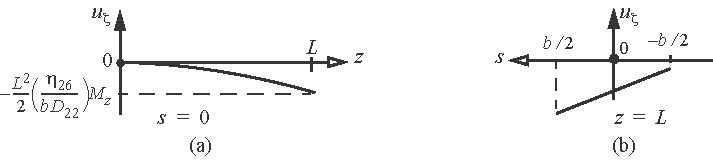
\includegraphics{Figure_8-14.pdf}}
\caption{Lateral displacement of the bar under torsion: (a) in the plane $s = \textbf{0}$, and (b) in the plane $z = L$.\label{fig8.14}}\vspace*{-10pt}
\end{figure}

\processfigure{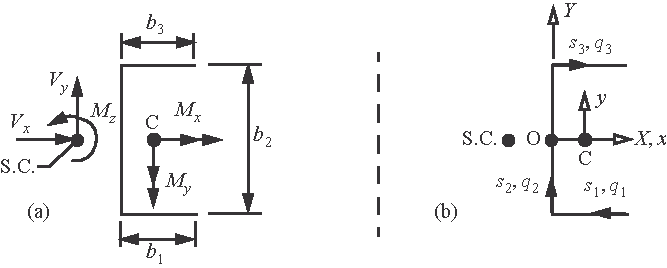
\includegraphics{Figure_8-15.pdf}}{\caption{a) Channel section subject to transverse bending and torsion. (b) Cross-sectional coordinate systems and shear flows.}\label{fig8.15}}

\begin{example*}[Transverse bending and torsion of a composite
channel section]\label{ex8.5}The cross section of the bar shown in
figure. \ref{fig8.15}(a) is composed of a lower horizontal flange with
length ${b_{1}=16\,\mathrm{mm}}$, an upper horizontal flange with
length $b_{3}=16\,\mathrm{mm}$. The flanges are joined by a
vertical web\vadjust{\vspace*{3pt}\pagebreak} with length $b_{2}=32\,\mathrm{mm}$. The lower flange
is denoted by branch 1, the web by branch 2, and the upper flange
by branch 3. Each branch is fabricated from T300/5208
graphite/epoxy with material properties listed in Table~\ref{tab8.2} on
page \pageref{tab8.2}, and the dimensional units used in this example are
Newtons and millimeters. The laminate in each branch consists of
eight plies with a specially orthotropic, symmetric stacking
sequence of $\left[45^{\circ}/-45^{\circ}/ 0/ 90\right]_{S}$.
The thickness of each branch $t=1.016\,\mathrm{mm}$. As shown in
figure. \ref{fig8.15}(b), the cross section is symmetric about the
\textit{X}-axis both in geometry and material properties. The
axial stiffness per unit length \textit{B} is given in
eq.~(\ref{eq8.46}), the torsional stiffness per unit length
$B_{s}$ is given in eq.~(\ref{eq8.47}), and they are the same in
each branch. For a specially orthotropic laminate the coupling
coefficient $b = 0$ in eq.~(\ref{eq8.46}). Numerical evaluation of
these stiffness coefficients are
\begin{align*}
B=A_{22}-A_{12} A_{21}/ A_{11}=15,822.7\,\mathrm{N}/\,\mathrm{mm}\mbox{, and }B_{s}=A_{66}=5,565.23\,\mathrm{N}/\,\mathrm{mm}.
\end{align*}
The section shown in figure~\ref{fig8.15}(a) is subject to an axial force \textit{N} (not shown in figure~\ref{fig8.15}(a)), transverse shear forces $V_x$ and $V_y$, bending moments $M_x$ and $M_y$, and a torque $M_z$.
\begin{enumerate}[a)]
\item[a)] Determine the material law for extension and bending of the
bar.
\item[b)] Determine the material law for shear and torsion of the
bar.
\end{enumerate}
\subsubsection{Solution to part (a).} The parametric equations of the contour in the \textit{X-Y}
coordinates are
\begin{gather*}
X_{1}\left(s_{1}\right)=b_{1}-s_{1} \quad Y_{1}=-b_{2}/ 2 \quad 0 \leq s_{1} \leq b_{1},\\
X_{2}\left(s_{2}\right)=0 \quad Y_{2}\left(s_{2}\right)=-b_{2}/
2+s_{2} \quad 0 \leq s_{2} \leq b_{2}\mbox{, and}\\
X_{3}\left(s_{3}\right)=s_{3} \quad Y_{3}=b_{2}/ 2 \quad 0 \leq
s_{3} \leq b_{3}.
\end{gather*}
To locate the modulus-weighted centroid on the \textit{X}-axis, we
first have to determine the modulus-weighted area $S$ and the
modulus-weighted first area moment about the \textit{Y}-axis
$S_{Y}$ from eq.~(\ref{eq8.52}). These are given by
\begin{gather*}
S=\int_{0}^{b_{1}} B d s_{1}+\int_{0}^{b_{2}} B d
s_{2}+\int_{0}^{b_{3}} B d
s_{3}=B\left(b_{1}+b_{2}+b_{3}\right)=1.01265 \times 10^{6}
\mathrm{~N}\mbox{, and }\\
S_{Y}=\int_{0}^{b_{1}} B
X_{1}\left(s_{1}\right) d s_{1}+\int_{0}^{b_{2}} B
X_{2}\left(s_{2}\right) d s_{2}+\int_{0}^{b_{3}} B
X_{3}\left(s_{3}\right) d s_{3}=B\left(b_{1}^{2}+b_{3}^{2}\right)
/ 2=4.05061 \times 10^{6}\,\textrm{N-mm}.
\end{gather*}
The location of the modulus-weighted centroid (\ref{eq8.53}) is
\begin{gather*}
X_{c}=S_{Y}/
S=\frac{b_{1}^{2}+b_{3}^{2}}{2\left(b_{1}+b_{2}+b_{3}\right)}=4
\mathrm{~mm} \quad Y_{c}=0.
\end{gather*}
The parametric equations of the contour with respect to the
centroidal axes $x$ and y are determined as follows:
\begin{gather}
x_{1}\left(s_{1}\right)=X_{1}\left(s_{1}\right)-X_{c}=12
\mathrm{~mm}-s_{1} \quad y_{1}=-16\,\mathrm{mm} \quad 0 \leq s_{1}
\leq 16\,\mathrm{mm}\tag{a}\label{ex8.5a}\\
x_{2}\left(s_{2}\right)=-4
\mathrm{~mm} \quad y_{2}\left(s_{2}\right)=-16\,\mathrm{mm}+s_{2}
\quad 0 \leq s_{2} \leq 32\,\mathrm{mm}\tag{b}\label{ex8.5b}\\
x_{3}\left(s_{3}\right)=-4\,\mathrm{mm}+s_{3} \quad y_{3}=16
\mathrm{~mm} \quad 0 \leq s_{3} \leq 16\,\mathrm{mm}\tag{c}\label{ex8.5c}
\end{gather}
Equations (\textbf{a}), (\textbf{b}), and (\textbf{c}) are
substituted into the formulas for the modulus-weighted second
moments $D_{x x}$ and $D_{y y}$ given by eq.~(\ref{eq8.57}) to get
\begin{gather}
D_{x x}=\int_{0}^{b_{1}} B y_{1}^{2} d s_{1}+\int_{0}^{b_{2}}
B y_{2}^{2} d s_{2}+\int_{0}^{b_{3}} B y_{3}^{2} d s_{3}=1.72826
\times 10^{8}\,\textrm{N-mm}^{2}\mbox{, and }\tag{d}\label{ex8.5d}\\
D_{y
y}=\int_{0}^{b_{1}} B x_{1}^{2} d s_{1}+\int_{0}^{b_{2}} B
x_{2}^{2} d s_{2}+\int_{0}^{b_{3}} B x_{3}^{2} d s_{3}=0.27004
\times 10^{8}\,\textrm{N-mm}^{2}.\tag{e}\label{ex8.5e}
\end{gather}
The
modulus-weighted product moment $D_{x y}=0$, because the $x$-axis
is an axis of symmetry. The cross-sectional material law in
extension and bending is
\begin{align}
\left[\begin{array}{@{}c@{}}N\\
M_{x}\\
M_{y}\end{array}\right]=\left[\begin{array}{@{}ccc@{}}S & 0 & 0\\
0 & D_{x x} & 0\\
0 & 0 & D_{y
y}\end{array}\right]\left[\begin{array}{@{}l@{}}
\frac{d w}{d z}\\
[4pt]
\frac{d \phi_{x}}{d z}\\
[4pt]
\frac{d \phi_{y}}{dz}\end{array}\right]=10^{6}\left[\begin{array}{@{}ccc@{}}1.01265
\mathrm{~N} & 0 & 0\\
0 & 172.826\,\textrm{N-mm}^{2} & 0\\
0 & 0 & 27.004\,\textrm{N-mm}^{2}\end{array}\right]\left[\begin{array}{@{}c@{}}\frac{d
w}{d z}\\[4pt]
\frac{d \phi_{x}}{d z}\\[4pt]
\frac{d \phi_{y}}{d
z}\end{array}\right].\tag{f}\label{ex8.5f}
\end{align}

\vspace*{-1pc}

\subsubsection{Solution to part (b).} To establish the material law for shear and torsion we start with
the shear flow given by eq.~(\ref{eq8.113}). For the channel
section the product moment $D_{x y}=0$, which means coefficients
$n_{x}=n_{y}=0$ and $k=1$ in eqs. (\ref{eq8.59}) and
(\ref{eq8.69}). At the contour origin where $s_{1}=0$ the shear
flow must equal zero since the longitudinal edge is free of
traction. Equation (\ref{eq8.113}) for each branch reduces to
\begin{align}
q_{j}\!\left(s_{j}\right)=-S_{x j}\!\left(s_{j}\right)
\frac{V_{y}}{D_{x x}}-S_{y j}\!\left(s_{j}\right) \frac{V_{x}}{D_{y
y}} \quad 0 \leq s_{j} \leq b_{j} \quad j=1,2,3.\tag{g}\label{ex8.5g}
\end{align}
The
modulus-weighted, first area moments $S_{x}$ and $S_{y}$ are
functions of the contour coordinate given by eq.~(\ref{eq8.70}),
and have dimensional units of \textit{N-mm}. The first area moment
functions with respect to the $x$-axis are
\begin{gather}
S_{x 1}\!\left(s_{1}\right)=\int_{0}^{s_{1}} B y_{1} d
s_{1}=-253{,}163 s_{1} \quad 0 \leq s_{1} \leq 16\,\mathrm{mm},\tag{h}\label{ex8.5h}\\
S_{x 2}\left(s_{2}\right)=S_{x 1}(16)+\int_{0}^{s_{2}} B
y_{2} d s_{2}=-4.05061 \times 10^{6}-253{,}163 s_{2}+7{,}911.34
s_{2}^{2} \quad 0 \leq s_{2} \leq 32\,\mathrm{mm}\mbox{, and}\tag{i}\label{ex8.5i}\\
S_{x 3}\left(s_{3}\right)=S_{x 2}(32)+\int_{0}^{s_{3}} B_{3}
y_{3} d s_{3}=-4.05061 \times 10^{6}+253{,}163. s_{3} \quad 0 \leq
s_{3} \leq 16\,\mathrm{mm}.\tag{j}\label{ex8.5j}
\end{gather}
Note that at the free
longitudinal edges $S_{x 1}(0)=0$ and $S_{x 3}(16)=-4.05061 \times
10^{6}+4.05061 \times 10^{6}=0$. The first area moment functions
with respect to the $y$-axis are
\begin{gather}
S_{y 1}\left(s_{1}\right)=\int_{0}^{s_{1}}\! B x_{1} d
s_{1}=189,872. s_{1}-7,911.34 s_{1}^{2} \quad 0 \leq s_{1} \leq
16\,\mathrm{mm},\tag{k}\label{ex8.5k}\\
S_{y_{2}}\left(s_{2}\right)=S_{y
1}(16)+\int_{0}^{s_{2}}\! B x_{2} d s_{2}=1.01265 \times
10^{6}-63,290.7 s_{2} \quad 0 \leq s_{2} \leq 32\,\mathrm{mm}\mbox{, and }\tag{l}\label{ex8.5l}\\
S_{y 3}\left(s_{3}\right)=S_{y
2}(32)+\int_{0}^{s_{3}}\! B_{3} x_{3} d s_{3}=-1.01265 \times
10^{6}-63,290.7 s_{3}+7,911.34 s_{3}^{2} \quad 0 \leq s_{3} \leq
16\,\mathrm{mm}.\tag{m}\label{ex8.5m}
\end{gather}
\vspace*{3pt}
\clearpage

\noindent Also note that $S_{y 1}(0)=0$ and $S_{y
3}(16)=0$. The resultant of the shear flow distribution is a
horizontal force denoted by $F_{X}$, a vertical force $F_{Y}$, and
a torque at the shear center $M_{z}$. The resultant forces are
\begin{align}\tag{n}\label{ex8.5n}
F_{X}=\int_{0}^{b_{3}}\! q_{3} d s_{3}-\int_{0}^{b_{1}}\! q_{1} d
s_{1}=\frac{V_{x}}{2}+\frac{3}{16}
V_{y}-\left(-\frac{V_{2}}{2}+\frac{3}{16} V_{y}\right)=V_{x}\mbox{, and }F_{Y}=\int_{0}^{b_{2}}\! q_{2} d s_{2}=V_{y}.
\end{align}
Equation (\textbf{\ref{ex8.5n}}) yields the expected result that the horizontal force
equals the shear force $V_{x}$, and the vertical force equals the
shear force $V_{y}$. We cannot compute the torque until the
location of the shear center is known. The coordinates of the
shear center $\left(x_{s c}, y_{s c}\right)$ are determined by
letting $I_{x x} \rightarrow D_{x x}$, $I_{y y} \rightarrow D_{y
y}$, $\bar{Q}_{x}(s) \rightarrow \bar{S}_{x}(s)$, and
$\bar{Q}_{y}(s) \rightarrow \bar{S}_{y}(s)$ in eq.~(\ref{eq3.106})
on page \pageref{eq3.106}. The transformation of eq.~(\ref{eq3.106}) to the
composite laminate is
\begin{align}
x_{s c}=-\left(\frac{k}{D_{x x}}\right) \int_{c} r_{n c}(s)
\bar{S}_{x}(s) d s \quad y_{s c}=\left(\frac{k}{D_{y y}}\right)
\int_{c} r_{n c}(s) \bar{S}_{y}(s) d s.\tag{o}\label{ex8.5o}
\end{align}
The coordinate normal
to the contour with respect to the centroid is denoted by $r_{n
c}(s)$. It is depicted in figure~\ref{fig3.3}(b) on page \pageref{fig3.3}, and the
expression to compute it is given in eq.~(\ref{eq3.11}) on page
\pageref{eq3.11}. For the channel section the normal coordinates for each branch
are
\begin{align}
r_{n c i}=x_{i} \frac{d y_{i}}{d s_{i}}-y_{i} \frac{d
x_{i}}{d s_{i}} \quad i=1,2,3.\tag{p}\label{ex8.5p}
\end{align}
Evaluation of eq. (\textbf{\ref{ex8.5p}})
results in $r_{n c 1}=-16\,\mathrm{mm}$, $r_{n c 2}=-4
\mathrm{~mm}$, and $r_{n c 3}=-16\,\mathrm{mm}$. For the channel
section in this example the evaluation of eq. (\textbf{\ref{ex8.5o}}) is
\begin{align}
x_{s c}=\left(\frac{-1}{D_{x x}}\right) \sum_{i=1}^{3}
\int^{b_i}_{0}r_{\textit{nci}} S_{x i} d s_{i}=-10\,\mathrm{mm} \quad
y_{sc}=\left(\frac{1}{D_{y y}}\right) \sum_{i=1}^{3} \int^{b_i}_{0}r_{\textit{nci}}S_{yi} d s_{i}=0.
\tag{q}\label{ex8.5q}
\end{align}
The torque from the shear flows with respect to the shear center is
\begin{align}
M_{z}=\sum_{i=1}^{3} \int^{b_i}_{0}r_{ni}q_i d s_{i},\tag{r}\label{ex8.5r}
\end{align}
where the coordinate normal to the contour with respect to the
shear center is denoted by $r_{n}(s)$. This normal coordinate is
depicted in figure~\ref{fig3.3}(b) on page \pageref{fig3.3}, and the expression to
compute it is given in eq.~(\ref{eq3.10}) on page \pageref{eq3.10}. For this
example the normal coordinate for each branch is given by
\begin{align}
r_{n i}=r_{n c i}-x_{s c} \frac{d y_{i}}{d s_{i}} \quad
i=1,2,3.\tag{s}\label{ex8.5s}
\end{align}
Evaluation of eq. (\textbf{\ref{ex8.5s}}) yields $r_{n 1}=-16
\mathrm{~mm}$, $r_{n 2}=6\,\mathrm{mm}$, and $r_{n 3}=-16
\mathrm{~mm}$. Evaluating the torque given by eq. (\textbf{\ref{ex8.5r}})
gives
\begin{align}
M_{z}=\underbrace{\left(8 V_{x}-3 V_{y}\right)}_{\text
{branch } 1}+\underbrace{\left(6 V_{y}\right)}_{\text {branch }
2}+\underbrace{\left(-8 V_{x}-3 V_{y}\right)}_{\text {branch }
3}=0.\tag{t}\label{ex8.5t}
\end{align}
Equation (\textbf{\ref{ex8.5t}}) shows that the torque due to the
shear flows equals zero at the shear center. Hence, the resultant
of the shear flow distribution is a force with its line of action
passing through the shear center having components $V_{x}$ and
$V_{y}$.

The material law for transverse shear relates the shear strains
$\psi_{x}$ and $\psi_{y}$ to the shear forces $V_{x}$ and $V_{y}$.
For the bar made of an homogeneous, isotropic material this
material law is discussed in article \ref{sec5.5.3} on page \pageref{sec5.5.3}. Referring
to eq.~(\ref{eq5.76}) the form of the material law is the same for
the composite material. That is,
\begin{align}
\left[\begin{array}{@{}l@{}}\psi_{x}\\
\psi_{y}\end{array}\right]=\left[\begin{array}{@{}cc@{}}c_{x x}
& c_{x y}\\
c_{y x} & c_{y
y}\end{array}\right]\left[\begin{array}{@{}l@{}}V_{x}\\
V_{y}\end{array}\right],\tag{u}\label{ex8.5u}
\end{align}
where the flexibility influence
coefficients $c_{x x}, c_{x y}, c_{y x}, \text { and } c_{y y}$
are determined from the complementary strain energy per unit axial
length $\bar{U}^{*}$. For the open section $\bar{U}^{*}$ is
obtained from eq.~(\ref{eq8.97}) on page \pageref{eq8.97}, and it is
\begin{align}
\bar{U}^{*}=\frac{1}{2} \int_{c} \frac{1}{A_{66}} q^{2} d s.\tag{v}\label{ex8.5v}
\end{align}
The shear strains $\psi_{x}$ and $\psi_{y}$ are determined
from derivatives of the complementary strain energy per unit axial
length with respect to the shear forces. For the channel section
in this example we get the following results:
\begin{gather}
\psi_{x}=\frac{\partial \bar{U}^{*}}{\partial
V_{x}}=\sum_{i=1}^{3}
\int^{b_i}_{0}
\frac{1}{\left(A_{66}\right)_{i}}
q_{i} \frac{\partial q_{i}}{\partial V_{x}} d s_{i}=
c_{xx}V_{x}+c_{x y} V_{y},\nonumber\\
\psi_{y}=\sum_{i=1}^3\int_{0}^{b_i}\frac{1}{(A_{66})_i}q_i\frac{\partial q_i}{\partial
V_{y}}ds_i=c_{yx}V_{x}+c_{yy} V_{y},\nonumber\\
c_{x x}=9.16404 \times 10^{6}\,\mathrm{N}^{-1} \quad c_{x
y}=c_{y x}=0 \quad c_{y y}=6.73827 \times 10^{-6}\,\mathrm{N}^{-1}.\tag{w}\label{ex8.5w}
\end{gather}

\vspace*{-1pc}

In general, external loads cause the bar to
resist a torque. For an open cross-sectional contour the shear
flows cannot provide this resistance to torsion. A separate
analysis for the linear elastic response to uniform torsion of a
symmetrically laminated bar was developed in article \ref{sec8.4}. The
result of this development is the material law (\ref{eq8.193})
that equates the torque to torsional stiffness $D_{T}$ times the
twist per unit length. The torsional stiffness is given by
eq.~(\ref{eq8.194}). To compute $D_{T}$ we evaluate the following
laminate properties:
\begin{itemize}
\item the transverse shear compliance (\ref{eq8.183})
$a_{44}=242.736 \times 10^{-6}\,\mathrm{mm}^{2}/\,\mathrm{N}$,

\item the torsional compliance (\ref{eq8.184}) $a_{66}=200.446
\times 10^{-6}\,\mathrm{mm}^{2}/\,\mathrm{N}$,

\item the bending
stiffness (\ref{eq8.161}) $D_{22}=1,130.94\,\textrm{N-mm}$,

\item the dimensionless
shear-extension coefficient in bending (\ref{eq8.162})
$\eta_{26}=-0.0459727$, and

\item the solution parameter
(\ref{eq8.190}) $\mu=2.82838\,\mathrm{mm}^{-1}$.
\end{itemize}
The function $g(\mu b/ 2)$ appearing in the equation for $D_{T}$ depends on
the length of the branch. For the channel section the values of
this function are
\begin{align}
g\left(\frac{\mu b_{1}}{2}\right)=g\left(\frac{\mu
b_{3}}{2}\right)=0.955805 \quad g\left(\frac{\mu
b_{2}}{2}\right)=0.977903.\tag{x}\label{ex8.5x}
\end{align}
The torsional stiffnesses for each
branch are
\begin{gather}
D_{T 1}=D_{T 3}=\frac{16 t^{3}}{3} \frac{g\left(\mu
\frac{16}{2}\right)}{a_{66}+\left[t^{3} \eta_{26}^{2} g\left(\mu
\frac{16}{2}\right)\right]/\left(3 D_{22}\right)}=26{,}589\,\textrm{N-mm}^{2}\mbox{, and }\tag{y}\label{ex8.5y}\\
D_{T 2}=\frac{32t^{3}}{3} \frac{g\left(\mu \frac{32}{2}\right)}{a_{66}+\left[t^{3}
\eta_{26}^{2} g\left(\mu \frac{32}{2}\right)\right]/\left(3
D_{22}\right)}=54{,}403.4\,\textrm{N-mm}^{2}.\tag{z}\label{ex8.5z}
\end{gather}
\vspace*{3pt}
\clearpage

\noindent The
torsional stiffness of the channel is equal to the sum of the
torsional stiffnesses of each of its branches. That~is,
\begin{align}
D_{T}=D_{T 1}+D_{T 2}+D_{T 3}=107,581.\,\textrm{N-mm}^{2}.\tag{aa}\label{ex8.5aa}
\end{align}
Finally, the material law for
transverse shear and torsion is
\begin{align*}
\left[\begin{array}{@{}c@{}}V_{x}\\
V_{y}\\
M_{z}\end{array}\right]=\left[\begin{array}{@{}ccc@{}}109{,}122.\,\mathrm{N} & 0 & 0\\
0 & 148{,}406.\,\mathrm{N} & 0\\
0 & 0 &
107{,}581.\,\textrm{N-mm}^{2}\end{array}\right]\left[\begin{array}{@{}c@{}}\psi_{x}\\
\psi_{y}\\
d \phi_{z}\\
d z\end{array}\right].\\[-60pt]
\end{align*}\hfill\qed
\end{example*}



%\vspace*{1.6pc}

\begin{thebibliography}{}
\bibitem{}
Canaday, H. ``Composites vs. Metals,'' in
\textit{\textbf{Aerospace America} \textit{}}53, no. 5, (May,
2015): 18--23.

\bibitem{}
Chandra, R., A. T. Stemple, and I. Chopra.``Thin-Walled Composite
Beams Under Bending, Torsional, and Extensional Loads.''
\textit{\textbf{Journal of Aircraft}} 27, no. 7 (July, 1990):
619--626.

\bibitem{}\label{Herakovich}
Herakovich, Carl T. \textit{\textbf{Mechanics of Fibrous
Composites}}. New York: John Wiley \& Sons, Inc., 1998.

\bibitem{}
Johnson, E. R., V. V. Vasiliev, V. V., and D. V. Vasiliev,
``Anisotropic Thin-Walled Beams with Closed Cross-Sectional
Contours.'' \textit{\textbf{AIAA Journal}} 39, no. 12 (2001):
2389--2393.

\bibitem{}
Lekhnitskii, S. G. \textit{\textbf{Theory of Elasticity of an
Anisotropic Body}}. Moscow: Mir Publishers, 1981, Sections 18--20, and 49.

\bibitem{}
Nixon, M. W. ``Extension-Twist Coupling of Composite Circular Tubes
with Application to Tilt Rotor Blade Design.'' \textit{Proceedings
of the 28th Structures, Structural Dynamics, and Materials
Conference} (Monterey, CA). Reston VA: American Institute of
Aeronautics and Astronautics, 1987, Part I: 295--303

\bibitem{}
Smith, E. C., and I. Chopra.``Formulation and Evaluation of an
Analytical Model for Composite Box-Beams.''
\textit{\textbf{Journal of the American Helicopter Society}} 36,
no. 3 (1991): 23--25.

\bibitem{}
Tsai, S. W. \textit{\textbf{Theory of Composites Design}}. Dayton
OH: THINK COMPOSITES, a division of ILT Corporation, 1992.

\bibitem{}
Vasiliev, V. V., and E. V. Morozov. \textit{\textbf{Advanced
Mechanics of Composite Materials and Structural Elements}}, 3d
ed., Waltham, MA: Elsevier, 2013, pp. 622--635.
\end{thebibliography}

\clearemptydoublepage

\end{document}